% Errors appear here 
\documentclass[
    11pt,
    a4paper,
    twoside,
    openright,
    fleqn,%
    parskip=half,%
    total={170mm,257mm},
    BCOR=5mm,
    DIV=10,
    footinclude=false%
    numbers=noenddot,
    cleardoublepage=empty]{scrbook}

% \documentclass[10pt,a4paper,twoside,openright,titlepage,fleqn,%
%     headinclude,,footinclude,BCOR5mm,%
%     numbers=noenddot,cleardoublepage=empty,%
%     tablecaptionabove]{scrreprt}
\usepackage{url}
\usepackage[utf8]{inputenc} 
\usepackage[T1]{fontenc} % this package magically allows symbol chars: `{}$^#` in listings
\usepackage{mathpazo} %-- use Palatino font
\usepackage{amsmath,amssymb,amsthm}
\usepackage[square]{natbib}
\usepackage{subcaption} 
\usepackage{xspace}
\usepackage[breaklinks=true,
            colorlinks=true,
            linktocpage=true,
            allcolors=colorforlinks]{hyperref} 
\usepackage[ruled,vlined,algochapter,linesnumbered]{algorithm2e}
\usepackage{calc}
\usepackage{ccicons} 
\usepackage{xspace} 
\usepackage{booktabs} 
\usepackage[english]{babel}  
\usepackage{listings}
\usepackage{scrhack} % ignore warnings about deprecated KOMA-Script
\usepackage[printonlyused,smaller,withpage]{acronym}
\usepackage[usenames,dvipsnames]{xcolor}
\usepackage{graphicx}
\usepackage{pdfpages}
\usepackage{todonotes}
\usepackage[shortlabels]{enumitem}
\usepackage{verbatim}
% [JF] added later by me 
% \usepackage{acro}
% \usepackage{acronym}

\usepackage[eulerchapternumbers,subfig,beramono,eulermath,pdfspacing,listings,dottedtoc]{classicthesis}
\usepackage{arsclassica}
\usepackage{geometry}
 \geometry{
 a4paper,
 total={140mm,230mm},
 left=30mm,
 top=30mm,
 }



\newcommand{\myName}{Jos Feenstra}
\newcommand{\myTitle}{Geofront: Library portability in a browser based visual programming language for geo-computation}

\newcommand{\myGroup}{3D geoinformation group}
\def\myGroupLogo{figs/tud-3dgeoinfo-black.png}
\newcommand{\myUni}{Delft University of Technology}

\newcommand{\myGraduationYear}{2022}
\newcommand{\myGraduationMonth}{June}

\newcommand{\mySupervisorOne}{Ir.\ Stelios Vitalis}
\newcommand{\mySupervisorTwo}{Dr.\ Ken Arroyo Ohori}
\newcommand{\mySupervisorThree}{Dr.\ Giorgio Agugiaro}
\newcommand{\myCoreader}{Dr.\ Hugo Ledoux}

%-- for names for \autoref commands
\def\chapterautorefname{Chapter}
\def\sectionautorefname{Section}
\def\subsectionautorefname{Section}
\def\subsubsectionautorefname{Section}
\def\algorithmautorefname{Algorithm}

% a way to make images fit the paper
% https://tex.stackexchange.com/questions/86350/includegraphics-maximum-width
\def\maxwidth{460pt} 


%-- for pdf metadata
\hypersetup{pdfauthor={\myName}}
\hypersetup{pdfkeywords={thesis, geomatics, TU Delft}}
\hypersetup{pdfsubject={A thesis submitted to the Delft University of Technology in partial fulfillment of the requirements for the degree of Master of Science in Geomatics}}
\hypersetup{pdftitle={\myTitle}}

%-- handy shortcuts
\newcommand{\ie}{i.e.}
\newcommand{\eg}{e.g.}
\newcommand{\reffig}[1]{Figure~\ref{#1}}
\newcommand{\refsec}[1]{Section~\ref{#1}}
\newcommand{\refchap}[1]{Chapter~\ref{#1}}

% [JF]: added a command to prettify this dodgy syntax. m stands for monospace
\newcommand{\m}[1]{\texttt{#1}}

%-- colours for the hyperlinks
\definecolor{colorforlinks}{RGB}{27, 60, 131}

\lstdefinestyle{note}
{
    breaklines=true, 
    basicstyle=\footnotesize,
    keywordstyle=\color{blue},
    commentstyle=\color[rgb]{0.13,0.54,0.13},
    backgroundcolor=\color{cyan!10},
}
\lstnewenvironment{note}
{\lstset{style=note}}
{}

% I keep changing the styling of geofront, so lets put them here
\newcommand{\geofront}{Geofront}

% I keep changing research questions, so lets put them here
% \newcommand{\myMainRQ}{\textit{How to design and implement a web-based vpl for geo-computation which supports running existing geo-computation libraries in a web browser?}}
\newcommand{\myMainRQ}{\textit{How can native geocomputation libraries be \emph{compiled}, \emph{loaded}, and \emph{utilized} within a browser-based dataflow-VPL?}}

\newcommand{\mySubRQOneTitle}{Representation} % previously: facilitation
% \newcommand{\mySubRQOne}{\textit{To what extent is a browser-based application able to facilitate a generic 3D geometry vpl?}}
\newcommand{\mySubRQOne}{\textit{How to implement a browser-based dataflow-vpl for processing 3D geometry?}}

% \newcommand{\mySubRQOne}{\textit{How to implement a visual programming environment in a browser which able to facilitate geo-computation?}}
\newcommand{\mySubRQTwoTitle}{Compilation}
\newcommand{\mySubRQTwo}{\textit{How can geocomputation libraries written in system-level languages be \textbf{compiled} for web consumption?}}
\newcommand{\mySubRQThreeTitle}{Loading}
\newcommand{\mySubRQThree}{\textit{To what extent can a web-consumable library be \textbf{loaded} into a web-vpl without explicit configuration?}}
\newcommand{\mySubRQFourTitle}{Utilization}
% \newcommand{\mySubRQFour}{\textit{What are the advantages and disadvantages of \textbf{using} an existing geoprocessing library through a geo-web-vpl, as opposed to native utilization of said library?}}
\newcommand{\mySubRQFour}{\textit{How can a 'geo-web-vpl' be \textbf{used} to create geodata pipelines?}}








% ********************************************************************
% listings from arsclassica
% ********************************************************************

\let\orgtheindex\theindex
\let\orgendtheindex\endtheindex
\def\theindex{%
	\def\twocolumn{\begin{multicols}{2}}%
	\def\onecolumn{}%
	\clearpage
	\orgtheindex
}
\def\endtheindex{%
	\end{multicols}%
	\orgendtheindex
}

\makeindex

% ********************************************************************
% listings
% ********************************************************************

\definecolor{lightergray}{gray}{0.99}

\lstset{language=[LaTeX]Tex,
    keywordstyle=\color{RoyalBlue},
    basicstyle=\normalfont\ttfamily,
    commentstyle=\color{Emerald}\ttfamily,
    stringstyle=\rmfamily,
    numbers=none,
    numberstyle=\scriptsize,
    stepnumber=5,
    numbersep=8pt,
    showstringspaces=false,
    breaklines=true,
    frameround=ftff,
    frame=lines,
    backgroundcolor=\color{lightergray}
} 

\lstset{morekeywords=%
        {function, f32, i32},
        commentstyle=\color{Emerald}\ttfamily,%
        frame=lines}

\lstset{basicstyle=\normalfont\ttfamily}
\lstset{flexiblecolumns=true}
\lstset{moredelim={[is][\normalfont\itshape]{/*}{*/}}}
\lstset{basicstyle=\normalfont\ttfamily}
\lstset{flexiblecolumns=false}
\lstset{moredelim={[is][\ttfamily]{!?}{?!}}} 
\lstset{escapeinside={£*}{*£}}
\lstset{firstnumber=last}
\lstset{moredelim={[is][\ttfamily]{!?}{?!}}}

\DeclareRobustCommand*{\pacchetto}[1]{{\normalfont\ttfamily#1}%
\index{Pacchetto!#1@\texttt{#1}}%
\index{#1@\texttt{#1}}}

\DeclareRobustCommand*{\bibtex}{\textsc{Bib}\TeX%
\index{bibtex@\textsc{Bib}\protect\TeX}%
}

\DeclareRobustCommand*{\amseuler}{\protect\AmS{} Euler%
\index{AmS Euler@\protect\AmS~Euler}%
\index{Font!AmS Euler@\protect\AmS~Euler}}

\lstnewenvironment{code}% 
{\setkeys{lst}{columns=fullflexible,keepspaces=true}%
\lstset{basicstyle=\small\ttfamily}%
}{}

\lstset{extendedchars} 
\lstnewenvironment{sidebyside}{% 
    \global\let\lst@intname\@empty 
    \setbox\z@=\hbox\bgroup 
    \setkeys{lst}{columns=fullflexible,% 
    linewidth=0.45\linewidth,keepspaces=true,%
    breaklines=true,% 
    breakindent=0pt,%
    boxpos=t,%
    basicstyle=\small\ttfamily
}% 
    \lst@BeginAlsoWriteFile{\jobname.tmp}% 
}{% 
    \lst@EndWriteFile\egroup 
        \begin{center}% 
            \begin{minipage}{0.45\linewidth}% 
                \hbox to\linewidth{\box\z@\hss} 
            \end{minipage}% 
            \qquad 
            \begin{minipage}{0.45\linewidth}%
            \setkeys{lst}{frame=none}% 
                \leavevmode \catcode`\^^M=5\relax 
                \small\input{\jobname.tmp}% 
            \end{minipage}% 
        \end{center}% 
} 

\lstset{numbers=left,
    numberstyle=\scriptsize,
    stepnumber=1,
    numbersep=8pt
}   

\setcapindent{1em} %-- for captions of Figures
% \setcounter{tocdepth}{\sectiontocdepth}

\subject{MSc thesis in Geomatics}
\title{\myTitle}
\author{\myName}
\date{\myGraduationMonth\xspace\myGraduationYear}
\publishers{A thesis submitted to the Delft University of Technology in partial fulfillment of the requirements for the degree of Master of Science in Geomatics}

\begin{document}
% \pagestyle{plain}

%******************************************************************
% Frontmatter
%******************************************************************
\frontmatter

%******************************************************************
% The cover page 
% (it needs to be manually edited and exported as a PDF)
% (see folder README.txt in folder 'cover')
% (I would not include it for the version you put in the repository)
%******************************************************************

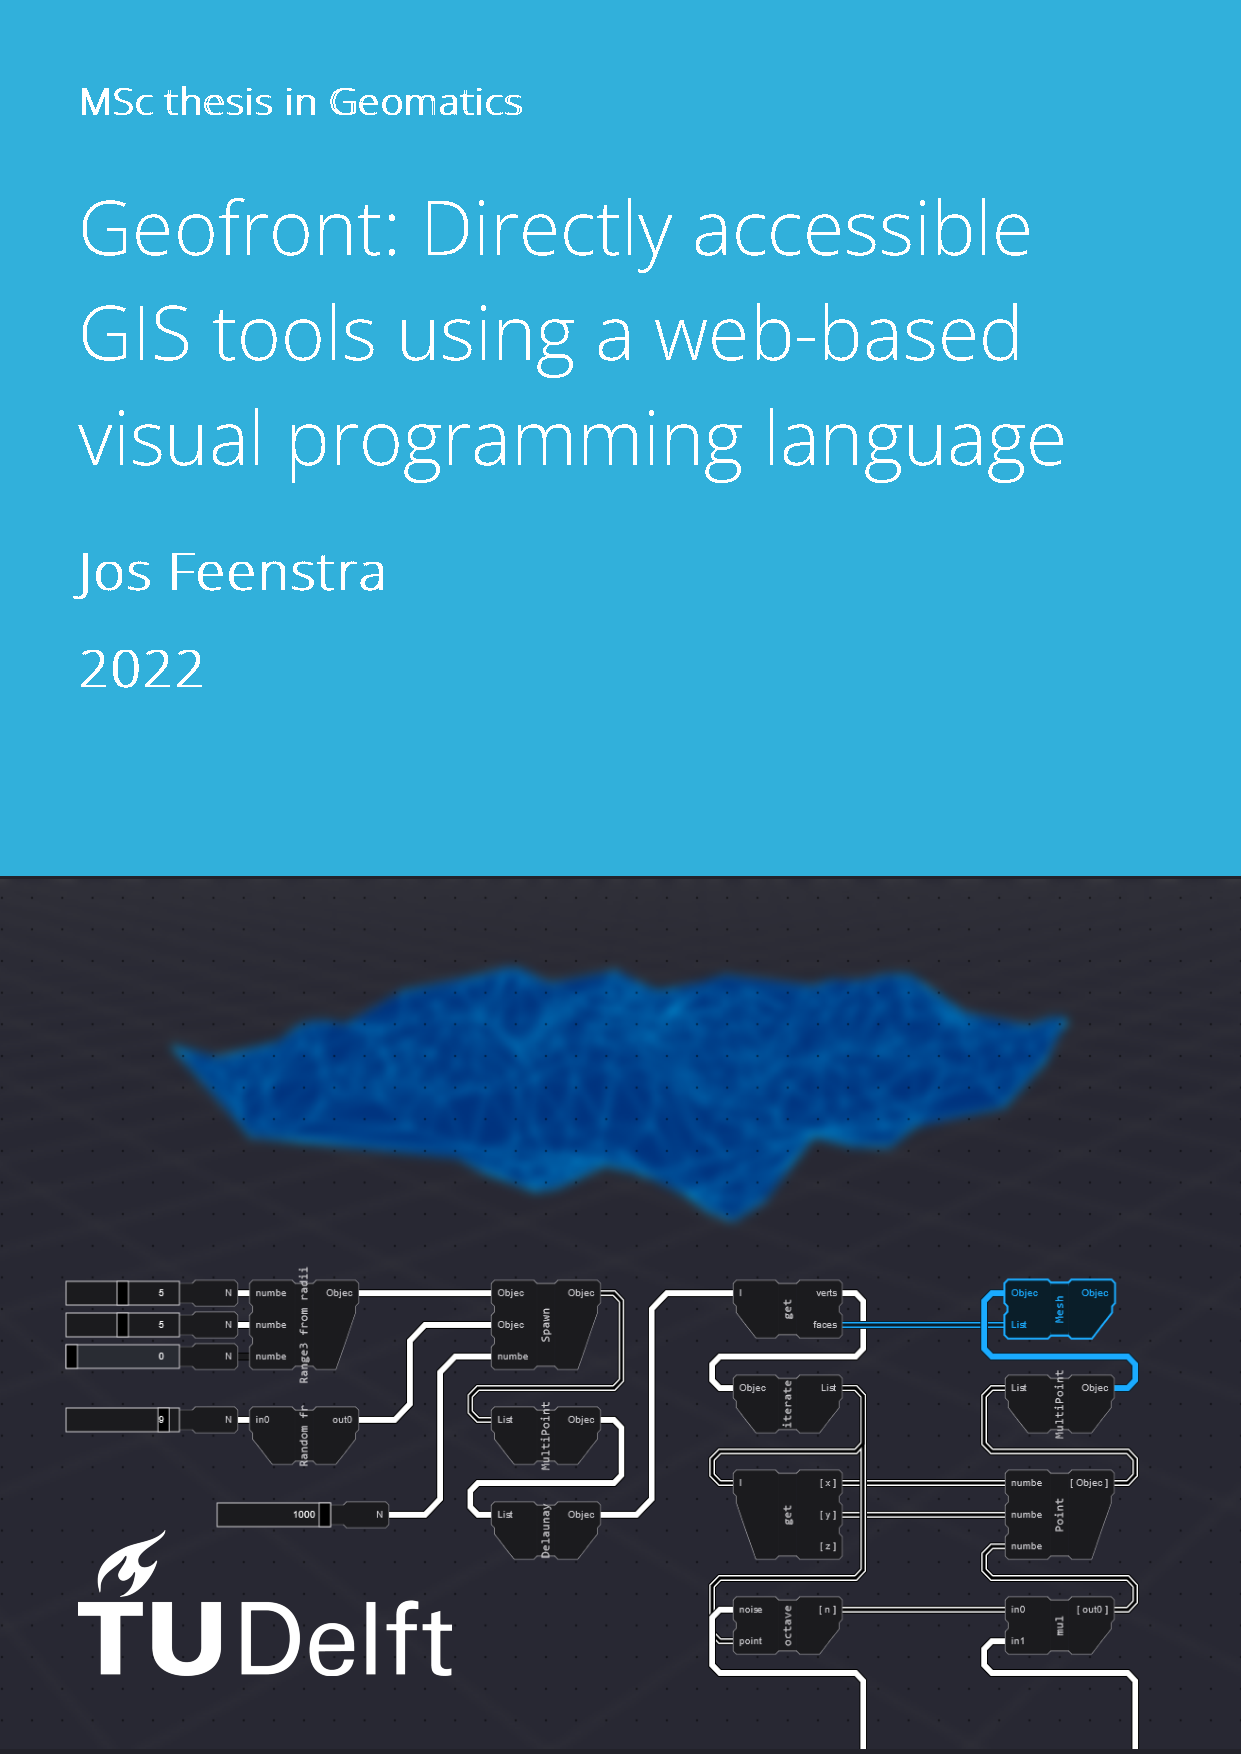
\includepdf{0-cover/cover_front.pdf}
\cleardoublepage

\maketitle[3]

% \clearpage
%!TEX root = ../thesis.tex

\thispagestyle{empty}

\hfill
\vfill

\noindent\myName: \textit{\myTitle} (\myGraduationYear)\\
\ccby\xspace This work is licensed under a Creative Commons Attribution 4.0 International License. To view a copy of this license, visit \url{http://creativecommons.org/licenses/by/4.0/}.

\vspace{3em}


\vspace{3em}

\noindent{} The work in this thesis was carried out in the:\\

\begin{tabular}{ll}
\parbox{0.3\textwidth}{\includegraphics[width=\linewidth]{\myGroupLogo}}
&
\parbox{0.7\textwidth}
{
  \myGroup\\
  \myUni\\
}       
\end{tabular}

\vspace{3em}
\noindent
\begin{tabular}{ll}
Supervisors:  &  \mySupervisorOne \\
              &  \mySupervisorTwo \\
Co-reader:    &  \myCoreader\\
\end{tabular}


\cleardoublepage
\chapter*{Abstract}

X is an essential part of any ...

The problem ...

The goal of this study is to

This study presents and prototypes a novel method which allows \ac{GIS} practitioners without a background in software development, to access the full potential of core transformation and analysis capabilities found in native \ac{GIS} libraries.

% That is based on visual programming, and static web applications. 


% The study attempts to meet this goal by designing and implementing a 
novel method based on the fields of visual programming, and static web applications. 

% The prior works on static geo-web applications and \ac{GIS} \ac{VPL}s indicate that a strong theoretical framework is in place.
% But, and this is especially evident in the prior studies regarding Browser-based geocomputation, the practical implementation of these theories were only partially successful, and limited in scope. 
% This necessitates a practical approach in response. 

A Prototype VPL was developed to host the functionalities of \ac{GIS} libraries from within an application, and in a composable manner. Additionally, it is used to connect these libraries to various \ac{GUI} features. 
The format of web application is used to allow this prototype to be directly accessible to end users without installation or configuration. 
% Geodata used within the application is also exclusively statically hosted geodata, or user-submitted data. 
This prototype is statically hosted, to minimize operational costs, and is equipped with WebAssembly, so that libraries written in native languages can be used without resorting to active backend web services. 
Finally, as this prototype is intended for \ac{GIS} usage, both scalability to handle sizable datasets, and rich \ac{GUI} support (3D viewers, file inputs, sliders, text boxes, graphs), are primary design considerations and assessment criteria.

Using this, ...

This method turned out to indeed provide solve

The significance of this method lies herein that it ...


% This method is thereafter used to load various \ac{GIS} libraries, and used in demo applications, after which an assessment can be made on its quality and the extend of its achieved functionalities. 
% The study concludes by addressing if the method meets the overarching goal.


% Geocomputation is a cornerstone of GIS \& modern mapping needs.
% While the last decades have seen major advancements, writing a geocomputational pipeline remains a complex, non-trivial exercise. 
% Performing geocomputations by utilizing a visual programming language (VPL) within a web browser is a novel development which seeks to simplify this process, allowing more people to write these types of pipelines more successfully.
% It would, in theory, allow end-users to author geocomputation pipelines, without the need of a software development background, and without the need to install software.
% utilizing a dataflow model.
% This model is the standard within VPLs dealing with geometry processing, and contains many advantages in terms of performance and reliability.

% In this context, the portability of existing geocomputation libraries is a common problem.
% This is often addressed by maintaining duplicate JavaScript alternatives to libraries such as GDAL, PROJ, and GEOS, complicating innovation.  

% This study seeks to improve the state of browser-based geocomputation VPLs by attempting to bring industry-standard geo-libraries to these environments. 
% The study poses that this can only be done if native geocomputation libraries can be \emph{compiled} to WebAssembly, \emph{loaded} into a VPL, and \emph{utilized} in a browser-based dataflow-VPL format.
% Discovering if and how these steps can be performed is the central question of this study. 
% % This study seeks to improve the state of web-based geocomputation VPLs 
% % by discovering if the library portability problem can be overcome, and if so, how.

% This question is answered by testing a possible solution.
% A proof of concept web-based VPL is designed, implemented and evaluated, which makes use of a novel plugin system, as well as a directed, acyclic graph-based data model \& interface.

% Using this proof of concept, the study was able to demonstrate that the web platform was sufficiently capable of representing a dataflow VPL capable of constructing geocomputation pipelines.
% The functional programming-properties of this dataflow VPL also makes geo-libraries sufficiently \emph{usable}, albeit with some well-known caveats of dataflow-VPLs, like the representation of conditionals and iteration.  

% The current methods of \emph{compiling} existing C++ geocomputation libraries to the web turned out to be insufficient for the purposes of this study.  
% This is due to the Emscripten compiler's focus on compiling full C++ applications instead of separate libraries. 
% Despite this, the study wás able to demonstrate how a novel method can be used to sufficiently \emph{compile} and \emph{load} multiple Rust-libraries for usage in the VPL, thanks to more feature-rich WebAssembly tools in the Rust ecosystem. 
% While Rusts geocomputation libraries are young, the study presents this method to either offer emscripten contributors a blueprint of a desired workflow, or to offer geocomputation library contributors a powerful use-case for the Rust language. 

% All in all, this means that either if the geocomputation libraries found in the Rust ecosystem mature, or if Emscripten's capabilities improve, then the code portability problem \& dataflow problem of existing web-based geocomputation VPLS can be solved. 


% \begin{note}

%     "make a simple narrative of what you did and what are the results."
%     "make it not be a very rough draft"
%     "6.2: deliver the things you promised."
%     "make it more formal: replace: "crucial", "by far" or "impressive""

%     Stelios Draft Comments
%     ======================
    
%     In general, I think it's going well. I think the intro is fine, although it can be improved. I like the conclusions quite a lot, tbh. You are giving proper and interesting answers to the raised questions. The rest is a bit of a very rough draft, as I see. So, some specific points:
    
%     TODO: Tone down stuff
%     -  It seems like you have placed several bits here and there that seem like either introduction or conclusions. I feel your enthusiasm and excitement in your writing, but I think you are bringing questions and answers in places were people would normally just expect a simple narrative of what you did and what are the results.
    
%     TODO: Write 6.2
%     -  Speaking of results, we are missing the experiments so please put this at your first priority. This is because it feels like you promise things that you do not deliver.
    
%     TODO: Find & Replace
%     -  In general, you are using some very bold statements and informal expressions. The latter is kinda okay, but the first one is very dangerous. I've noticed words like "crucial", "by far" or "impressive" which seem very biased and subjective, so better be avoided. You can still use them here and there (mostly in the conclusions), but I think you use them way  too much (again, I can see your enthusiasm).
    
%     TODO: Find & Replace 
%     -  Minor thing, but I think you have confused \citet with \citep. The first one is used when the citation is part of the sentence and the latter when it's at the end of a sentence (or in a parenthesis, anyway).
    
% \end{note}

% This might allow web based VPLs for geocomputation to be 
% Geodata computation is important.
% Geodata computation is difficult.
% geo-web-vpls could help, but have seen little research
% This study: design, implement, analyze a new prototype geo-web-vpl. 
% Design-> utilize existing, native libraries written in C++ \& Rust on the web, in the format of a vpl.

% results -> it works.

% -> study shows that interplay between textual and visual programming is possible


% \begin{note}
%  - Performance intensive: (Big data, O(n^2) problems) 
%  - Heterogenous data (type, quality, scale, criteria, crs) 
%  - Complex (geometric) operations (linalg, bundle adjustment, procedural modelling) 
% \end{note}

% All of this makes the process of geocomputation difficult. 


% The full flowchart runs client-side in a browser, and both end results and intermediate products can be inspected in a 3D viewer.

% GeoFront offers several functionalities such as the parametric creation of 2D and 3D primitives, triangulation, isocurve extraction, and more. 
% These functionalities can be expanded upon though a plugin system which utilizes the existing "Node Package Manager" infrastructure.
% Together with WebAssembly, this enables the utilization of industry standard geoprocessing libraries such as `CGAL`, `GDAL` and `PROJ`, and data parsing libraries such as `IFC.js` and `laz-rs`.



% Following the implementation, the project was tested by simulating use-case scenarios. 
% The tests demonstrate the feasibility of [...]
% At the same time some key parameters of [...] identified which if tuned properly they can optimize the performance, behavior and robustness of the geo-web-vpl.
% With the project being a prototype solution, the vpl is far from operational and there is certainly a lot of space for improvement regarding both components. 

% 1. Tryout (ACTUAL)
%    - A-la wapm WebAssembly Package Manager allows packages to be run from within the package-page itself. 
%   - Just meant to quickly try out some features.

% 2. Educational (ACTUAL)
%    - interactive educational tool
%    - (What does a delaunay triangulation look like? how does it behave? What happens if you lower the radius of inverse distance weighting ? )

% 3. Rapid-Prototyping (POSSIBLE)
%    - Setting up pipelines which can be consumed by cloud-based geoprocessing services. 
%    - Future work: export flowchart to a process which can be run natively or server side.

% 4. Publishing (POSSIBLE)
%    - Geotiff.io / ModelLab
%    - Web FME 
%    - Publish full web apps in and off themselves, making use of zero, one or multiple wasm-compiled libraries.  
%    - Future work: export to web-app (without flowchart)

% % Safesoft's FME, but web based \& open source 

% % CONCLUSION
% By creating geofront, this thesis was able to discover .............

% - The web is able to facilitate a visual proregramming language.

% - The web is able to be used for geoprocessing, albeit with some caveats
%   - TypedArrays,
%   - Geometric predicates 
%   - Rounding
%   - ETC.

% - Many of these things can be fixed with webassembly, but webassembly itself has other shortcomings
%   - Differences between Rust \& C++

% - reasonable performance 
%   (- great considering the platform)

% - would not be possible without these modern web features
%   - Web Assembly 
%   - Typed Array's 
%   - Web Workers
%   - Web Components,
%   - 2D Canvas API
%   - Web GL

% \todo{[JF]: I need to add more critical notes on promises of accessibility. Is a webapp truly accessible? Is a flowchart interactive, or does it hinder interactiveness? }

% I believe that such a web application can make geoprocessing more accessible to practitioners.
% This empowers users to create small geoprocessing demo's, and share these 
% With geofront, geoprocessing libraries can be loaded and used interactively. Users are also able to create and share flowcharts.
%%%%%%%%%%%%%%%%%%%%%%%%%%%%%%%%%%%%%%%%%%%%%%%%%%%%%%%%%%%%%%%%%%%%%%

% 


%%%%%



\begin{note}

  Lessons
  ==========
  
  - give yourself clear todo's per day. 
    Not too little, not too much.
    Upon completion, the day falls apart
  
  
  TODO
  ============
  
  high-level
  ----------
  
  [x] The intro / story needs to be altered 
      - stronger tie to Geo & web
      - VPL + Web
  
  [x] rewrite and balance research questions
  - [x] then trickle down the consequences of those changes throughout the thesis
  mid-level
  ---------
  
  [ ] TODO: rewrite abstract in accordance with new story

  [x] Deep dive in Hugo's comments, fix those aspects 
    - [x] sort acronyms
  
  [x] Add a stronger web-component in the introduction (presentation)
  [x] Add cloud native / cloud-based geodata component to the introduction  
  
  [ ] Cleanup Chapter 2 and 3.  
    - Some parts are still more relevant than other parts. 
    - Also, there are some things I say or use in chapter 4, 5, and 6, that were not properly explained in chapter 2. Examples of this are emscripten, or CGAL. 
    - However, a complete rewrite would be too much work.
    - Would love to hear your take on this.
  
  [ ] Make chapter 4 and 5 more streamlined 
    - I've noticed that I repeat myself quite often.
    - I think this is because I was not sure if I already said something relevant in the chapter before.
  
  [ ] Show your results more clearly, do the coding you have done justice
  
  [ ] finish chapter 6 properly 
    - Experiments: add a section on a use-case application, using potree + startin + geofront std + obj downloader
  
  [x] write stronger, more clear conclusions.
    - hmm, i think they are already quite clear. But again, this is to be reconsidered when the overall story of the thesis changes  
  
  low-level: thursday & friday
  -------------------

  - [ ] write 
  - [x] TODO: write Acknowledgements
  - [x] Add arsclassica template to the thesis
  - [x] Make the code snippets / listings work properly
  - [x] replace all code screenshot with proper listings
  - [ ] create all missing uml diagrams
  - [ ] add proper graphs for the data you've gathered 
  - [ ] Add all proper metadata to Zotero, for a nice bibliography
  - [ ] Fix all TODO graphics
  - [ ] Fix all acronyms,
  - [ ] Sort the acronyms at the end 
  - [ ] Make sure CiteT and citeP is properly used everywhere. No more raw 'et. al.' statments 
  - [ ] Capitalize all VPL / replace with acronyms
  - [ ] Sources need to be fixed (more data, check if I can do things like 'empscripten contributors')
  - [ ] Replace C++ into C / C++ everywhere, but especially the intro
  - [ ] appendix: software implementation & link to video
\end{note}


\chapter*{Acknowledgements}

\begin{itemize}
    \item Stelios
    \item Ken
    \item Martin, Current employer, GeoDelta 
    \item Sybren, Previous employer, Sfered
    \item Nadja
    \item Tim
    \item Friends \& Family
\end{itemize}

\ldots



 
\clearpage

\setcounter{tocdepth}{2}

\tableofcontents
\listoffigures
% \listoftables
% \listofalgorithms


\clearpage
\chapter*{Acronyms}

% thank you, vscode sort lines extension!
\begin{acronym}
    \acro{CDN}{Content Delivery Network}
    \acro{CGAL}{Computational Geometry Algorithms Library}
    \acro{CLI}{Command Line Interface}
    \acro{CRS}{Coordinate Reference System}
    \acro{DAG}{Directed Acyclic Graph}
    \acro{DEM}{Digital Elevation Model}
    \acro{DT}{Delaunay triangulation}
    \acro{DTM}{Digital Terrain Model}
    \acro{DSM}{Digital Surface Model}
    \acro{ETL}{Extract Transform Load}
    \acro{EUD}{End User Development}
    \acro{FOSS}{Free and Open Source Software}
    \acro{GDAL}{Geospatial Data Abstraction Library}
    \acro{geo-vpl}{geocomputation or geometry VPL}
    \acro{geocomputation}{Geospatial data computation}
    \acro{GEOS}{Geometry Engine Open Source}
    \acro{GIS}{Geographical Information Science}
    \acro{GUI}{Graphical User Interface}
    \acro{HTTP}{Hyper Text Transfer Protocol}
    \acro{IDE}{Integrated Development Environment}
    \acro{MVC}{Model View Controller}
    \acro{os}{operating system}
    \acro{OSGEO}{Open Source Geospatial Foundation}
    \acro{OGC}{Open Geospatial Consortium}
    \acro{TIN}{triangular irregular network}
    \acro{UI}{User Interface}
    \acro{UX}{User Experience}
    \acro{VD}{Voronoi diagram}
    \acro{VPL}{Visual Programming Language}
    \acro{W3C}{World Wide Web Consortium}
    \acro{wasm}{WebAssembly}
    \acro{WFS}{Web Feature Service}
    \acro{WMS}{Web Mapping Service}
    \acro{WPS}{Web Processing Service}
    % \acro{etl}{Extract Load Transform}
\end{acronym}


% WHY DOESNT THIS SHOW UP???
% https://tex.stackexchange.com/questions/557187/acronyms-in-a-table-environment-are-not-shown-in-the-list-of-acronyms


\cleardoublepage

%******************************************************************
% Mainmatter
%******************************************************************
\mainmatter

%-------------------------------------------------------------------------------------------------%
% An introduction in which the relevance of the project and its place in the 
% context of geomatics is described, along with a clearly-defined problem statement.
% [KEN]
% instead, I think you can start by saying that web applications are popular
% explain the benefits briefly
% apart from having no installation

% then, I think you can make a better argument for your thesis overall
% explain that historically, thin client fat server was the standard
% for the reasons you listed
% and then directly explain why this is potentially changing now

\newpage
\section{Introduction}

% Dissolving the discrepancy between visualization \& processing in web-apps.

% web is popular 
% geoweb-applications are popular 
% online geodata processing is popular 
% client-side geodata processing 


% STELIOS: Relatively slow
 
% show an example 

Interactive, browser-based \ac{gis} applications form an indispensable component of the modern geospatial software landscape. A web application is cross-platform in nature, and offers ease of maintainability and access, since no installment or app-store interaction is required to update or run the app. The ability be placed as a supplement within the larger context of a webpage is also not trivial. These features have made the browser a popular host for many \ac{gis} applications, especially when targeting end-users. 

% streamline these three paragraphs.
% I want something like -> problem: limitations. 

Despite the popularity of \ac{gis} web applications, the range of actual \ac{gis} abilities these applications are capable of is very limited. For example, \ac{geoprocessing}, like CRS translations, interpolation, boolean operations, or raster transformation kernels are usually not present within the same software environment as the web app. This limited range of capabilities limits the usefulness of \ac{gis} web applications, and with it the number of use cases a \ac{gis} web application can serve. Current geospatial web applications serve for the most part only as lightweight viewers; visualizers of pre-processed data. If web applications gain these functionalities, they could grow to be just as diverse and useful as desktop \ac{gis} applications. It would allow for a new range of interactive web applications, in which data users can post-process geodata quickly, uniquely, and on demand.

This raises the question of Why. Why are web \ac{gis} applications limited to just be viewers?

% This raises the question: why is this not done yet? two reasons 
% 1. People are content with server-side geoprocessing 
%    -> BUT: this does not serve every use-case 
% 2. Client-side geoprocessing is hindered by javascript and the web environment
%    -> NOT ANYMORE: WebAssembly
% 
% 
% To solve 2: WebAssembly
% To solve 1: We offer a case study which demonstrates a unique type of application which would not be possible without client-side geoprocessing. 

However, by making the functionality of an application not self-contained but distributed, 

The improvements of client-side hardware have opened up a second possibility: client-side geoprocessing, directly within a web application. By doing this, the hard divide between client visualization and server processing could be bridged.  while at the same time driving down the operational costs of geoprocessing servers. This is why client-side \ac{geoprocessing} in web applications is slowly gaining traction during the last decade \cite{kulawiak_analysis_2019, panidi_hybrid_2015, hamilton_client-side_2014}. 

% Interactive geospatial data manipulation and online geospatial data processing techniques are described as "current highly valuable trends in evolution of the Web mapping and Web GIS" \cite{panidi_hybrid_2015}. 

However, serious drawbacks to client-side geoprocessing where encountered during these studies. Browser-based geoprocessing suffers from the fact that it will need to be written in the `JavaScript` programming language. Previous attempts at client-side geoprocessing have shown that JavaScript based geoprocessing libraries do not offer the performance required for proper geodata processing \cite{hamilton_client-side_2014}. 
Moreover, the JavaScript library ecosystem does not offer viable alternatives to industry-standard libraries like CGAL and GDAL. 
% This would require alternatives to be rewritten in JavaScript, or would require the source code of mature libraries to be compiled to JavaScript. Both these solutions would be difficult to maintain, and would still end 
% Both these solutions contain many imperfections. The first option would be an inefficient, time-consuming task, and would mean code duplication. 
% The second option would mean taking C++-based libraries such as CGAL, and compiling them to a special, fast subset of JavaScript called `asm.js` using the `emscripten` compiler \cite{zakai_emscripten_2011}. 
% While this is more fast and reliable, it contains its own set of problems. 
% The generated, rather large JavaScript files usually take a long time to download, to scan, and to be properly optimized by a JavaScript Just In Time (JIT) Compiler \cite{haas_bringing_2017}. 

An emergent technology poses a solution to both problems. At the end of 2019, the \ac{w3c} officially pronounced WebAssembly as the fourth programming language of the web \cite{w3c_world_2019}. Since then, all major browsers have added official WebAssembly support. \ac{wasm} is a binary compilation target meant to be small, fast, containerized, and platform \& source independent \cite{haas_bringing_2017}. \ac{wasm} surpasses javascript in almost all performance aspects: it loads quicker, it is scanned quicker, and since it is close to bytecode, it can often run at a speed comparable to system level programming languages like C++ and Rust \cite{jangda_not_2019}. 

% \cite{beilschmidt_vat_2017}


% Related studies concerned with the performance of WebAssembly, together with the existing software around WebAssembly, pose enough evidence to suggest  theoretically possible (SOURCE: Emscriptem). 
% However, this leaves the question whether it is practically possible unanswered, evident by the fact that no wasm-powered geoprocessing tools exists at the time of writing this study. 

\newpage

% stelios: Speed up 

\subsection{Problem}

If WebAssembly performs as described by \cite{haas_bringing_2017} and \cite{jangda_not_2019}, it could theoretically be the missing link to make client-side geoprocessing viable. However, no wasm-powered geoprocessing tools exists yet at the time of writing. Hypothetically, this is because of two reasons. Firstly, WebAssembly brings along many practical uncertainties:

\begin{itemize}
  \item Do geoprocessing libraries directly compile into WebAssembly? If not, which workarounds are needed? 
  \item Will a \ac{wagl} load efficiently, or should they be split up into parts, and loaded lazily? 
  \item How well do \ac{wagl} operations perform in a browser, compared to their native counterparts? What can be done to make this difference as small as possible?
\end{itemize}

Secondly, the way geoprocessing is supposed to be performed within the context of a web-browser remains unknown. The above list of implementation considerations cover only how \ac{wagl}'s can be \emph{run}. Potential answers do not indicate how \ac{wagl}'s can be \emph{used}. \cite{jangda_not_2019} warns against assessing WebAssembly in a vacuum, and notes how its performance is highly dependent on the way it is used, and the context in which it is used. This context of geoprocessing within a web-browser brings up many considerations as well: 

\begin{itemize}
  \item How will users upload or specify the input in a web-browser?
  \item Can the transformations offered by \ac{wagl}'s be used like functions? Or do they require special services, such as a wrapper library, virtual file system, or a virtual Command line interface? 
  \item How can users recieve and evaluate the output in a web-browser?
  \item How can a sequence of geoprocessing steps be chained together in a web-browser?
  \item How can a web-based \ac{ui} or \ac{gui} facilitate all these functionalities?
\end{itemize}

These two sets of unknowns are highly dependent upon each other. Together, they form a barrier preventing further development of client-side geoprocessing. Since no wasm-powered, client-side geoprocessing application exist yet, there is no way to answer these questions, and no way to confirm the theoretical benefits of WebAssembly for client-side geoprocessing, and the geospatial community at large.



\subsection{Use Case}
% mini methodolody??


in order to demonstrate 

visual programming language.




%-------------------------------------------------------------------------------------------------%
\newpage

%-------------------------------------------------------------------------------------------------%
\subsection{Research Questions}

This study intends to discover if contemporary web technologies can facilitate client-side geoprocessing by seeking an answer to the following question:  

\textit{How to \textbf{design and create} a browser-based GIS environment which can \textbf{effectively utilize} \textbf{existing geoprocessing libraries}, using only the \textbf{current state} of \textbf{standard client-side web technologies}?}

\subsubsection*{Explanation}

% The research question is written purposefully written in the "how well does X support Y question" shape. To unpack its components: 

- \textbf{design and create}: The wording 'design and create' is used to signal that this will consider the theoretical design , as well as the practicalities of creating this design. 

- \textbf{Standard client-side web technologies}: This phrase is meant to limit the scope to only the standard, core technologies of major browsers (Chrome, Edge, Safari, Firefox). This means the four languages \ac{wasm}, CSS, JavaScript and HTML. Additionally, HTML5 gives us WebGl, the 2d Canvas API, SVG's, and Web Components to work with.

- \textbf{Current state}: The study will use contemporary, even bleeding edge features of the modern web, but its findings will nonetheless be bound to this time of writing, as web technologies in particular quickly change. 

- \textbf{Existing geoprocessing libraries}. This wording expresses this studies desire to explore the usage of existing geoprocessing libraries, rather than to recreate geoprocessing libraries from scratch.

- \textbf{Effectively utilize}: The study intends to not only find out how \ac{wagl}'s can be \textit{run} in a browser, but also how \ac{wagl}'s can be \textit{used}. 


\subsubsection*{Sub Questions}

The following sub-research questions are needed in order to answer the main question. The methodology chapter will explain the choices of these sub-questions. 

\textit{1 : What is the most fitting methodology of compiling C++ geoprocessing libraries to WebAssembly?}

\textit{2 : How to design and create a client-side geoprocessing interface for data-users?}

\textit{3 : How can wasm-compiled geoprocessing libraries be distributed and used in a client-side geoprocessing interface?}

\textit{4 : What are the advantages and disadvantages of GIS applications created using a client-side geoprocessing environment powered by WebAssembly?}

\newpage
\subsubsection*{Assessment}

At the final conclusion of the proposed thesis, we can answer if the designed and created GIS environment can indeed effectively utilize these geo-libraries.
this will be answered by quantitative and qualitative means:

Quantity
\begin{itemize}
    \item Have all required features been implemented?
    \item Which libraries can be used?
    \item What are the load \& run times of these libraries, compared to native execution?
\end{itemize} 

Quality
\begin{itemize}
    \item Have all design goals been met?
    \item Can data users 'effectively' handle input, process and output?
    \item Can the load \& run times be regarded as acceptable to use? 
\end{itemize} 


% ----
\subsection{Scope}


\subsection*{Will Include}

The 'will include' scope is represented by the Methodology chapter. 

%-----------------------------------------------------------------------------%
\subsection*{Will not include}

\subsubsection*{Server-side or Native WebAssembly} % **Client-side WebAssembly Only**

This study will limit itself to the \emph{client-side} usage of WebAssembly. 
A powerful case can be made for \emph{server-side}, or native level usage of WebAssembly, especially in conjunction with a programming language such as Rust. 
Rust compiled to WebAssembly could, compared to using python, java or C++, make geoprocessing more maintainable and reliable, while at the same time ensuring memory safety, security, and performance \cite{clack_standardizing_2019}. 

Server-side or native wasm is beyond the scope of this paper, but would be an excellent starting point for future work. Note that this also means that research into \ac{wagl}'s is important for more than just client-side geoprocessing. All geoprocessing could benefit from it.



\subsubsection*{Web Processing Service} % Will not be dealing with WPS 

% offered as server-side geoprocessing services.  
Similarly, this study will exclude the OGC standard of the \ac{wps} \cite{ogc_web_2015}, since these services do not offer \emph{client} side geoprocessing, but instead offer \emph{server} side geoprocessing. A client-side application \textit{could} create an interface to use such a service, to essentially offer geoprocessing to clients, but this study regards a solution like that as a workaround, not a true solution to the problem of client-side geoprocessing. 

This is not to say that client-side geoprocessing replaces the need for \ac{wps}. 
future work could research the possibility of utilizing a hybrid strategy of both client-side and server-side geoprocessing, following in the footsteps of \cite{panidi_hybrid_2015}. 

% Still, We must briefly discuss the \ac{wps}, since it seems to offer a solution to the problems addressed.

%The OGC standard of the \ac{wps} offers a set of protocols to standardize geoprocessing on a server. By specifying input data and instructions to one of these services, polling the status of the process, and then downloading the results once finished, a user can process geodata on a server. If a client-side application creates an interface to use such a service, it can essentially offer client-side geoprocessing.

% While this is more like a workaround for client-side geoprocessing than a solution, it can nonetheless be preferred. A Web Processing Service is an excellent solution when client-side hardware is limited, and when server-side resources are abundant. It is also more efficient if the datasets required for geoprocessing are already located on these servers, and when working with geo-datasets too large to store locally. 

% situational cuts both ways 

% a \ac{wps} do not replace the need for client-side geoprocessing, for much of the same reasons a \ac{wps} does not replace the need for native \ac{gis} applications like QGIS or ArcGIS.  

% The usefulness of a \ac{wps} is, just like client-side geoprocessing, situational. 

% For much of the same reasons \ac{wps} does not replace the 


% reasoning from the perspective of client-side geoprocessing, a \ac{wps} does not offer a true solution to the problem of client-side geoprocessing, but only a workaround. 


% When the reverse is true however, and when the application needs to remain interactive and responsive, other solutions are required.

% While 

% Future work could research the possibility of utilizing a hybrid strategy of both client-side and server-side geoprocessing, following in the footsteps of \cite{panidi_hybrid_2015}. 


\subsubsection*{Usability Analysis} % 

While usability is a major component of this research, no claims will be made that the developed use-case is more usable to native GIS applications or geoprocessing methods. This research attempts to solve practical inhibitions in order to discover whether or not client-side is \emph{an} usable option. If it turns out that this method is viable technically, future research will be needed to definitively proof \emph{how} usable it is compared to all other existing methods.  

% This paper seeks to first close this gap, limiting itself to overcoming the technical and design boundaries in the pursuit of practical client-side geoprocessing.

Similarly, a survey analyzing how users experience client-side geoprocessing in comparison to native geoprocessing must also be left to subsequent research. While this would gain us tremendous insight, client-side geoprocessing is too new to make a balanced comparison. Native environments like GRASSGIS, QGIS, FME or ArcGIS simply have a twenty year lead in research and development. 

%-------------------------------------------------------------------------------------------------%
% A related work section in which the relevant literature is presented and 
% linked to the project. 
% It should show that you clearly know the problem you plan to solve, 
% and that you master the related work. 

\chapter{Background}
\label{chap:background}

\begin{figure}
  \centering
  \graphicspath{ {../../assets/diagrams/} }
  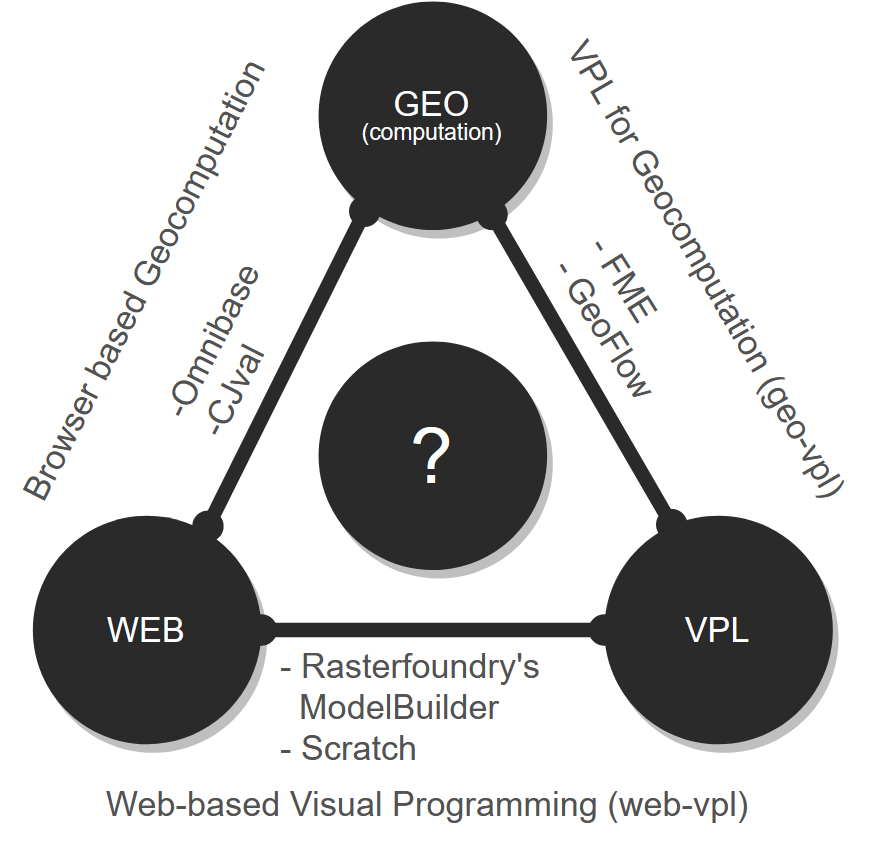
\includegraphics[width=270px]{geo-web-vpl.png}
  \caption{Triangle Model}
  \label{fig:triangle-model}
\end{figure}

This chapter offers an overview of the theoretical background that this study builds upon.
The study takes place at the intersection of three prior bodies of work,  represented by the corners of \reffig{fig:triangle-model}:
\begin{enumerate}[-]
  \item \refsec{sec:background-geo} covers the background on Geocomputation
  \item \refsec{sec:background-web} covers the background on Web applications
  \item \refsec{sec:background-vpl} covers the background on Visual Programming Languages
\end{enumerate}
Each one of these cornerstones will be discussed and analyzed by themselves, after which \refchap{chap:related} and \refchap{chap:methodology} will focus on the interplay and connections between these bodies of work. 

\section{Geocomputation}
\label{sec:background-geo}

\begin{note}
  TODO: finish this chapter
\end{note}

This section offers a brief background on the wide topic of geocomputation. 

% PURPOSE: Show that you understand geo-computation | Show why the rest of the study will focus on the computer graphics side of things

Geocomputation is a central component of the wider field of geo-informatics. 
The term geocomputation, or geodata processing, is used to represent all types of computations performed on geographical data. 
Anything from the calculation of an area of a polygon, to \ac{crs} transformations, feature overlay, or converting a raster dataset into a vectorized dataset, is regarded as geocomputation.

It must be emphasized that a geocomputational procedure is always fully defined by and dependent upon its input and output data types (similar to any type of computation). 
This is also why geocomputation is seldom a \emph{goal} in itself, but much rather the \emph{means} to discovering geo-information. 

\begin{note}
  TODO: show images of geo-computation
\end{note}

\subsection{Similarities and differences with neighboring fields}

\begin{figure}
  \centering
  \graphicspath{ {../../assets/diagrams/} }
  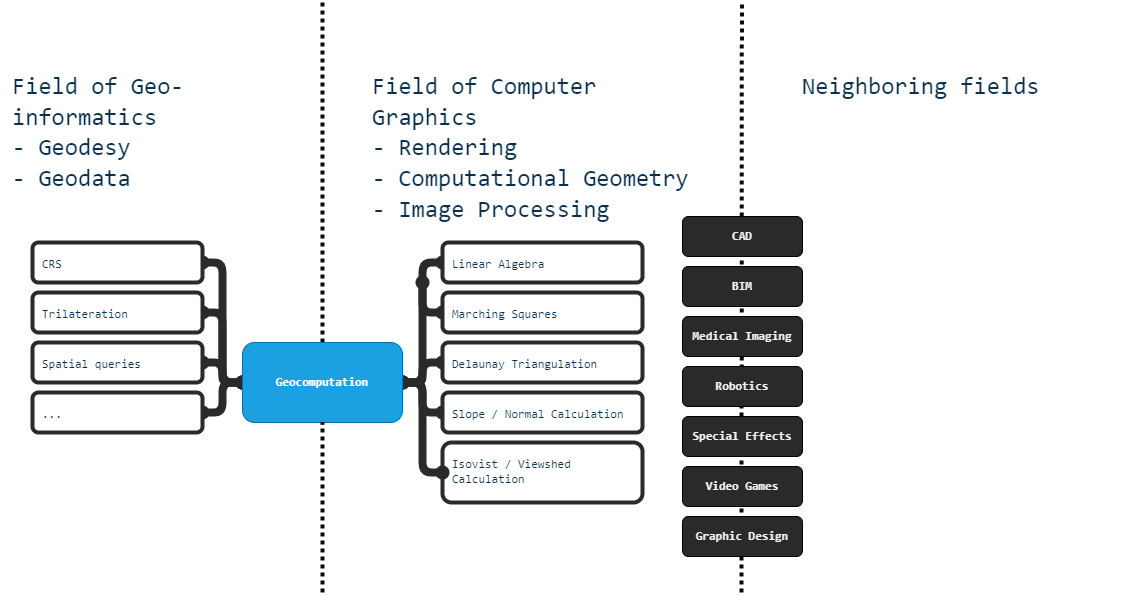
\includegraphics[width=380px]{geocomputation.png}
  \caption{Geocomputation in relation to other fields}
  \label{fig:geocomputation}
\end{figure}

Geocomputation can be seen as an applied field of the more general field of computer graphics. 
Other applications of computer graphics include computer aided design (CAD), Building Information Modelling (BIM), molecular biology, medical imaging, robotics, but also special effects, video games, and graphic design.
For this reason, these applied fields can be regarded as neighbors to geocomputation \& GIS. 

It is important to recognize that certain geocomputational procedures fully overlap with computer graphics and these neighboring fields, while others are very specific to the field of GIS and geo-informatics.
As an example, matrix transformations and reprojections are commonplace in the wider field of computer graphics, but transformations formalized and structured in the form of \ac*{crs} is very specific to the field of GIS (See \reffig{fig:geocomputation}).
As such, geocomputational procedures can roughly be categorized in two fields: 
\begin{itemize}[-]
  \item geocomputations \emph{specific} to \ac{gis},
  \item \emph{common} computational geometry procedures
\end{itemize}
This categorization can be identified by noting if an operation appears in a neighboring field, or just in the field of \ac{gis}.

This \emph{specific} category exists because of \ac{gis}s foundation in the field of Geodesy, and the nature of geographical data. 
Geodata differentiates itself from any form of data by its sizable nature, and geospatial nature. 
GIS dataset sizes easily scale into terabytes of data, and each datum specifically represent a real, measured, earthly phenomenon.
This makes storage and accuracy more relevant than other computer graphics applications. 

% NOTE TO SELF: GIVE CATEGORIES OF GEOCOMPUTATION IF IT IS ASKED FOR, OTHERWISE, LEAVE IT
% \subsection{Categories of Geocomputation}

% Geocomputation is a very broadly defined phenomenon, used to represent a great variety of computations. 
% To give an overview of this variety, a hierarchical subdivision of different types of geocomputation can be given, based on a subdivision of geodata types.

% The following distinctions are made between different geodata types:
% \begin{itemize}
%   \item Uniform
%   \subitem Rasters (Imagery)
%   \subitem Hexagons
%   \item Irregular, Vector-based
%   \subitem TIN 
%   \subitem solids
%   \subitem 3D Tiles
%   \item Semantic geodata:
%   \subitem Tabular geodata (QGIS)
%   \subitem Hierarchical, 'object oriented' geodata (GML / JSON) 
%   \item Point-cloud
% \end{itemize}

% Corresponding geocomputations are typically grouped together with one of these types of data. 
% However, this taxonomy is not perfect, since many computations exist \emph{between} between two different types of geodata.

% \subsubsection{Raster Geocomputation}

% - image processing
% - transformation kernels 

% \subsubsection{Vector Geocomputation}


% \subsubsection{Semantic Geocomputation}
% \begin{enumerate}[-]
%   \item often raster or vector at the core, with semantics layered on top 
% \end{enumerate}

% - 
% - 

% \subsubsection{Pointcloud Geocomputation}

\subsection{Geocomputation libraries}

\begin{figure}
  \centering
  \graphicspath{ {../../assets/images/background} }
  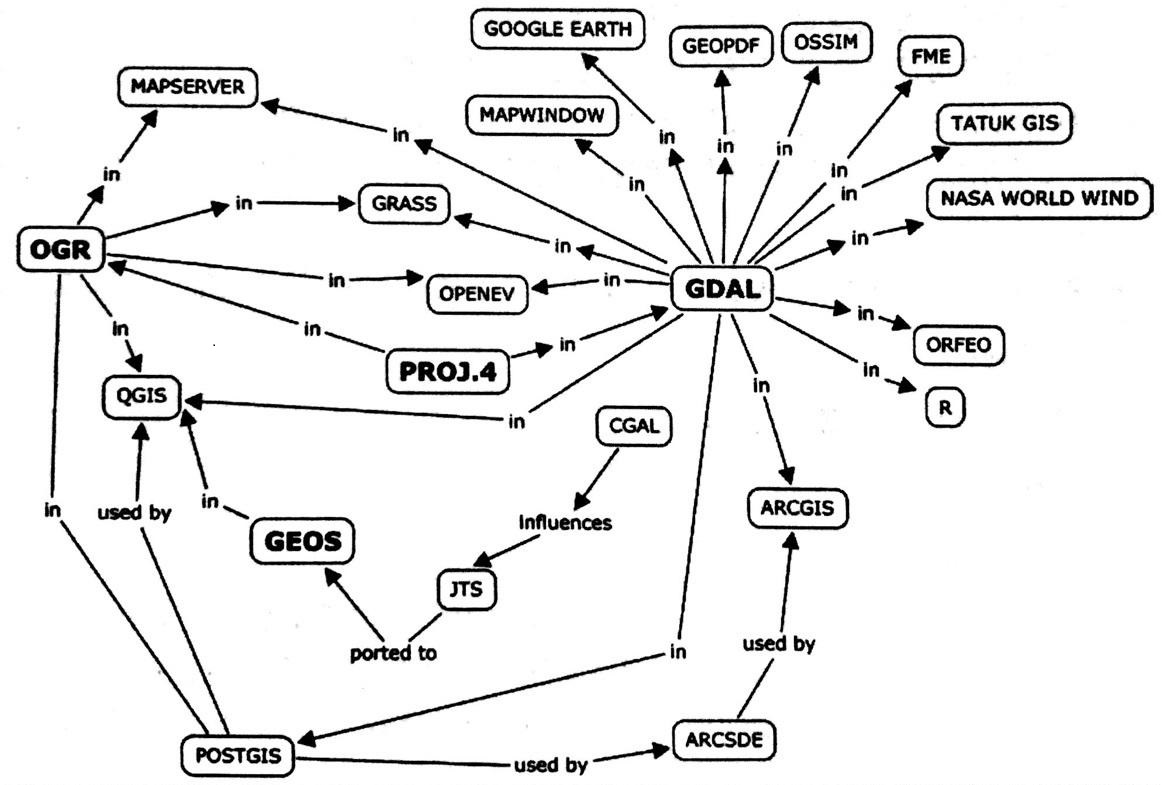
\includegraphics[width=380px]{all-geo-libraries-explained.jpg}
  \caption{Dependency graph of common geocomputation libraries. (This needs validation) }
  \label{fig:geolib-dependencies}
\end{figure}

Numerous geocomputational software libraries exist, written in a plethora of programming languages. 
Still, a certain 'Canon' can be defined based on popularity in terms of numbers of downloads, numbers of contributors, and number of dependent projects.  

Out of all open-source geocomputational libraries, the ones developed and maintained by the \ac{osgeo} (Source) can be regarded as the most significant to the field of \ac{gis}. 
These libraries include:
\begin{itemize}[]
  \item The \ac{gdal} (Source) 
  \item The Cartographic Projections and Coordinate Transformations Library titled PROJ (Source)
  \item The Geometry Engine Open Source (GEOS) (Source)
\end{itemize}
The geocomputations found in these libraries operate primarily on 2D / 2.5D raster and Simple Feature datasets (Source).
How these projects related together is presented by \reffig{fig:geolib-dependencies}.
Together, these libraries represent the core computational needs specific to the field of \ac{gis}. 

For the more common computational geometry needs, the \ac{cgal} library is also widely used.

% Almost all popular GIS end-user applications have these libraries at their core, such as 

\subsection{Conclusion}

The Take-away: 

Combination of general computational geometry, and computations very specific to GIS.

Geocomputation is mostly facilitated by a very select number of C++ libraries. 

\newpage

\section{Frontend web applications}
\label{sec:background-web}

\begin{note}
  TODO: this chapter is too large, the client-server / front-back elements should be trimmed down, or maybe even entirely removed. I think Its too granular. 

  Also, add more pictures!
\end{note}

This section offers a background on frontend web applications.
Since this topic is too large in scope to fully cover, three elements are chosen which are highly relevant to this study.
Finally, these three topics are linked to each other in \refsec{sec:background-web-conclusion}.

\subsection{Distributed systems}
\label{sec:background-web-terminology}

In software development of distributed systems, the following phrases exist: 
\begin{enumerate}[-]
  \item Client and Server 
  \item Frontend and backend
  \item Native application and web application
  \item web application and website
\end{enumerate}
While these phrases do overlap to an extend, years of interchangeable usage have lead to their differences often being overlooked. 
This study wishes to shed light on the relationships between these phenomena, as the nuances between them are vital to this studies contribution.

\subsubsection*{The client-server model}

\begin{figure}
  \centering
  \graphicspath{ {../../assets/images/misc/} }
  
\includegraphics[width=380px]{todo.jpg}
  \caption{A typical client-server interaction) }
  \label{fig:client-server}
\end{figure}

First, the client-server model. 
The client-server model refers to a distributed application architecture which balances storage and processing responsibilities between two cooperating types of programs: 
Clients and servers.
In this model, a client sends a request to a server, and the server provides the response asked for (see \reffig{fig:client-server}).
While this model immediately invokes images of web clients and web servers, it is important to recognize that the client-server model is far older than either web applications, or the World Wide Web in general. 
It is an abstract computational model, of which the World Wide Web is just one example.
A corresponding client and server may even exist on the same machine. 
A program running on a machine can act as a client, a server, or both, based on the role this program sets out to fulfill in relationship to other programs. 

The client-server model is beneficial for sharing resources, both in terms of storage and processing. 
A distinction is made between centralized models, in which the bulk of these resources are centralized on one or more servers, and decentralized models, which distribute and offload some or all of the computational resources to the clients. 
A centralized model has the advantage of making clients simple and interchangeable, at the cost of making them highly reliant on the uptake of and connection to the server. This also generates more client-server traffic. 
A decentralized model makes clients independent and decreases traffic, at the cost of the complications caused by decentralized architectures. 
The choice between a centralized or decentralized client-server model is therefore highly reliant on the resources of client and server hardware, as well as the quality of the connection between the server and client.  

\subsubsection*{Frontend and backend}

The terms frontend and backend, though closely related to clients and servers, refer to different phenomenon. 
Both are separations of concerns, a design principle prevalent in computer science to specialize a program into separate responsibilities. 
However, client and server programs are defined by their separation into "requester" and "responder" roles, whereas the frontend and backend are defined by their separation into "presentation" and "data access" functions. 
Presentation functions are responsible for interacting with the end-user of the application, and is concerned with aspects such as user interface, user interaction, and rendering.
"data access" interacts with the physical hardware of the machine, and is concerned with aspects such as storage methods, database management, and scalability.  
It just so happens that the presentation functions often corresponds with a requester role,
and that data access functions often corresponds with the responder role.
However, this is never a given. 
A server can be responsible for providing both the frontend and backend functionality, in the case the presentation of an application is rendered on this server. 

\subsubsection*{Native application and web application}

The nuances between a web application and a native application must also be specified, alongside their relationship to clients and servers. 
In this context, we make a distinction between \emph{Programs}, which refer to individual processes on either the side of the client or the server, and an \emph{application}, which either represents a non-distributed, self contained program, or represents the whole of corresponding client and server programs together.
Client programs or server programs are also often abbreviated as clients and servers.  
If a client runs without the corresponding server it relies upon, we can say that the client functions, but the entire \emph{application} does not function. 
In practice, however, the term 'web app' often specifically refers to the client, confusingly enough.

In any case, a program is considered native if it directly runs on the operating system of a device.
A program is considered web-based or browser-based if a browser is required to run it. 
A web application always has a client, as it will always need to be initially served by a corresponding server.
However, the extend to which the functionality of a web app is self contained or continuously reliant on this server may vary.
A native program may also be a client, as there is nothing preventing a native program of making the exact same web request as a web application. 

Due to this ambiguity of 'client-side' being able to refer to both native and web clients, this study makes use of the terminology 'browser-based programs' or 'browser-based applications', to point to web clients in particular. 

Web applications have specific advantages and disadvantages compared to native applications. 
The big advantages are that web applications are cross-platform by nature, and offer ease of accessibility, since no installment or app-store interaction is required to run or update the app (src: vpl 2019, src: hybrid).
As soon as a web app is found, it can theoretically be used.
The containerized nature of the web also makes web applications in general more safe. 
For unknown native applications there is always a danger of installing malicious software, whereas an unknown web application without any privileges is practically harmless (Needs citation). 
The ability to share the a functional application with a link, or to embed it within the larger context of a webpage, is also not a trivial advantage.

The disadvantage is that normally, web applications can only be written in JavaScript, a very-high level interpreted programming language. 
Its high-level nature leads to imprecision in using computational resources. 
For example, it makes no distinction between integer and floating point arithmetic.  
Additionally, the safety and containerization demands of the web make web applications more removed from the operating system and hardware.
Any type of \ac{os} interaction such as opening a window, interacting with the file system, or drawing directly to the screen buffer, is off-limits.  
Both these layers of indirection makes web applications traditionally unfavorable for demanding, highly specialized programs. 

\subsubsection*{Web application and website}

Lastly, a soft distinction is also made between websites, and web applications. 
Roughly speaking, a web application is a website which requires javascript in order to be functional.
This makes websites more static, and web applications more dynamic, being able to change based on user input.  
Wikipedia (Source) can be considered a website, whereas overleaf (Source) is definitively a web application. 
Many border cases also exist, like Twitter (Source).
Following the above definition, twitter is a web application, despite the fact that its core functionalities could be implemented without any client-side javascript.

\begin{note}
  Sources: 

  (https://en.wikipedia.org/wiki/Web_application, bad source, but this is more 'conventional wisdom' than true 'knowledge', couldn't find a more credible source, 
  
  what would make a person credible on this content?)
  
  (https://en.wikipedia.org/wiki/Frontend_and_backend)
\end{note}


\subsection{Rich Clients}
\label{sec:background-web-rich}

In the early days of the World Wide Web, web applications were practically impossible, and the web consisted of websites exclusively. 
Then, with the introduction of the javascript scripting language in 199x (Source), and browser plugins like Adobe Flash (Source), the first couple of web application slowly started to be developed. 
Still, these early web applications exclusively used a centralized client-server model.
The clients were simple, and completely reliant on the server. 

In the decades that followed, the javascript runtime of web browsers saw continuous improvements, alongside additions like HTML5, facilitating more interactive usage of webpages.
As the web and web technologies matures, new ways of using these technologies are discovered.
Web applications became more interactive, and frontend functionalities were slowly moved from the server to the client. 

These developments continued.
Since 2012, a trend of \textbf{rich web-clients} can be widely recognized \cite{hamilton_client-side_2014, panidi_hybrid_2015, kulawiak_analysis_2019}.
At that point, the browser had become powerful enough to allow for more decentralized client-server models.
By reducing servers to just static file servers, and adding all routing and rendering responsibilities to the client, the interactivity of a web application could be maximized. 
This model was dubbed "single page application", and was and still is facilitated by javascript frameworks like Angular, React and Vue.
However, the real facilitator of these developments are the browsers vendors themselves, as these frameworks would not be possible without the performance increase of javascript. 

This growth has also lead to web applications being used 'natively'. 
Tools like Electron (Source) allow web applications to be installed and 'run' on native machines by rendering them inside of a stripped down browser. 
Many contemporary 'native' applications work like this, such as VS Code, Slack, and Discord.
Additionally, tools like React Native (Source) are able to compile a web application into a native application without a browser runtime.  

If the applications resulting from both types of tools are to be regarded as 'web apps' or 'native apps', is left as an exercise to the reader. 
In any case, it becomes clear that rich web clients and their build tooling are starting to blur the line between native and web software.

\subsection{WebAssembly}
\label{sec:background-wasm}

If the line between web application and native application was already starting to get blurry, WebAssembly makes this line almost invisible. 
From all browser-based features, WebAssembly turned out to be a deciding factor of this study. This makes it important to be aware of the state of WebAssembly and its performance considerations.

\ac{wasm} is officially dubbed the fourth type of programming language supported by all major web browsers, next to HTML, CSS, and JavaScript.
Strictly speaking however, WebAssembly not a language, but a binary instruction format for a stack-based virtual machine.
(SOURCE: https://webassembly.org/)
it can be used to, theoretically, run any application or library in a web browser, regardless of the language used to create it, be it C/C++, Python, C\#, Java, or Rust. 
This means that in order to create a web application, developers can now in principle develop a normal, native application instead, which can then be compiled to WebAssembly, and served on the web just like any other web application. 

\subsubsection*{Limitations}

The sentence above uses the phrase \emph{in principle}, since there are quite a few caveats to the format. 
While in theory any application can be compiled to WebAssembly, in practice, not all applications turn into functional webassembly applications, due to certain factors.
These limitations can be split up into two groups: 
Limitations due to the web platform, and limitations due to the current state of the language and its host.

First of all, WebAssembly is required to adhere to the same containerization restrictions as javascript and the web at large. 
There is no '\m{os}' or '\m{sys}' it can call out to, as it cannot ask for resources which could be a potential security risk, like the file system.
Secondly, WebAssembly is in its early phases as a language, and is intended as a simple, bare-bones, low-level compile target. 
For example, the current version does not support concurrency features like multithreading.

Many of these shortcomings can be mitigated by calling JavaScript and HTML5 features from WebAssembly. 
This is what the majority of current WebAssembly projects look like. 
However, this layer of javascript 'boilerplate' or 'glue code' is inefficient, as it leads to duplication and redirection.
Additionally, platforms wishing to support WebAssembly must now also support javascript. 

\subsubsection*{Performance}

The initial performance benchmarks look promising. The majority of performance comparisons show that WebAssembly only takes 10\% longer than the native binary it was compared to \cite{haas_bringing_2017}. A later study confirms this by reproducing these benchmarks \cite{jangda_not_2019}. It even notices that improvements have been made in the two years between the studies. However, Jangda et. al. criticize the methodology of these benchmarks, stating that only small scale, scientific operations where benchmarked, each containing only 100 lines of code. The paper then continues to show WebAssembly is much more inefficient and inconsistent when it comes to larger applications which use IO operations and contain less-optimized code. These applications turn out to be up to twice as slow compared to native, according to their own, custom benchmarks. 
Jangda et. al. reason that some of this performance difference will disappear the more mature and adopted WebAssembly becomes, but state that WebAssembly has some unavoidable performance penalties as well. 
One of these penalties is the extra translation step, shown in \reffig{fig:wasm-trajectory}, which is indeed unavoidable when utilizing an in-between compilation target. 

Some studies have taken place evaluating \ac{wasm}'s performance for geospatial operations specifically. 
Melch performed extensive benchmarks on polygon simplification algorithms written in both javascript and WebAssembly \cite{melch_performance_2019}. 
It concludes by showing WebAssembly was not always faster, but considerably more consistent. 
Melch had this to say: "To call the WebAssembly code the coordinates will first have to be stored in a linear memory object. 
With short run times this overhead can exceed the performance gain through WebAssembly. 
The pure algorithm run time was always shorter with WebAssembly.". 
These findings match \cite{jangda_not_2019}, showing that the duplication of data into the webassembly memory buffer is a considerable bottleneck.

A recent study concerned with watershed delineation \cite{sit_optimized_2019} also concluded client-side WebAssembly to be more performant than server-side C, which, as a side effect, enabled their application to be published on the web without an active server. 

Lastly, the sparse matrix research of Sandhu et al. will be mentioned. \cite{sandhu_sparse_2018}. It shows again that WebAssembly's performance gain is most notable when performing scientific computations. it states: "For JavaScript, we observed that the best performing browser demonstrated a slowdown of only 2.2x to 5.8x versus C. Somewhat surprisingly, for WebAssembly, we observed similar or better performance as compared to C, for the best performing browser.". It also shows how certain preconceptions must be disregarded during research. For example, it turned out that for WebAssembly and JavaScript, double-precision arithmetic was more performant than single-precision, probably due to byte spacing.

Even though this study falls in the category of scientific computation, these performance considerations will still have to be taken into account. The most important conclusion to to take away from prior research on WebAssembly is that \ac{wasm} must not be regarded as a 'drop-in replacement', as \cite{melch_performance_2019} puts it. Just like any language, WebAssembly has strengths and weaknesses. While \ac{wasm} is designed to be as unassumptious and unopinionated about its source language as possible, the implementations of host environments do favor certain programming patterns and data structures over others, and this will have to be taken into account when using the compile target.

\begin{figure}[!tbp]
  \centering
  \begin{minipage}[b]{0.80\textwidth}
    \graphicspath{ {../../assets/images/misc/} }
    
\includegraphics[width=300px]{todo.jpg}
    \caption{Comparison of compilation trajectories}
    % based on the finding of \cite{jangda_not_2019}
    \label{fig:wasm-trajectory}
  \end{minipage}
\end{figure}

% \subsubsection{Background}

% The original paper on WebAssembly was published on June 14, 2017 \cite{haas_bringing_2017}. The authors write that the reason behind the creation of WebAssembly is the observation that certain web applications started using JavaScript as a compile target, using a high-performance subset of JavaScript called 'asm.js' \cite{mozilla_asmjs_2013}. However, JavaScript remains a high-level, highly abstract programming language, which never intended to be used as a compile target. The discrepancy between intended use and actual use led to many complications for developers using JavaScript this way, but also for the developers of JavaScript itself \cite{haas_bringing_2017}. 
% In order to relieve javascript of the responsibility of being a 'low-level' compilation target, developers of the four major browser vendors Mozilla, Google, Apple and Microsoft created WebAssembly and its corresponding paper, in a joined effort.

% This paper starts by promising WebAssembly as a save, fast, portable and compact compilation target. It continues by showing how previous attempts at low-level code on the web fail in at least one of these criteria, and that WebAssembly is the first to deliver on all of them. The follow up chapters cover a proof of memory safety, a proof of soundness of the language design, and the design decisions which had to be made to live up to those four criteria. These details will become relevant to the proposed thesis when reasoning about why WebAssembly might be faster in one case versus another.

% \subsubsection*{Adoption \& Implementation}

% not in a vaccuum

% On 5 December 2019, the \ac{w3c} officially pronounced WebAssembly as the fourth programming language of the web \cite{w3c_world_2019}. Philippe Le Hégaret, the \ac{w3c} Project Lead, writes “The arrival of WebAssembly expands the range of applications that can be achieved by simply using Open Web Platform technologies. In a world where machine learning and Artificial Intelligence become more and more common, it is important to enable high performance applications on the Web, without compromising the safety of the users,”. Since then, most major browsers have added official WebAssembly support.

% As of writing this proposal, WebAssembly has of yet not seen widespread adoption in web developer communities. Opinions deviate, but in general, WebAssembly is considered a niche technology, often being named as 'experimental' and 'bleeding edge'. 

% This would explain why, to the best of the author's knowledge, not many projects and papers explicitly link WebAssembly and GIS. Papers on \ac{wasm} do state \textit{"3d data transformations and visualization"} as some of the examples of a high performance web applications \cite{haas_bringing_2017, jangda_not_2019}. What's more, certain GIS applications, like Google Earth, have started to use WebAssembly, as seen in \reffig{fig:google-earth} \cite{google_google_2020}. How it is used is unknown due to the engine being closed-source, but it is speculated that \ac{wasm} is used to access code written for the original C++-based desktop application.

% \begin{figure}[!tbp]
%   \centering
%   \begin{minipage}[b]{0.80\textwidth}
%     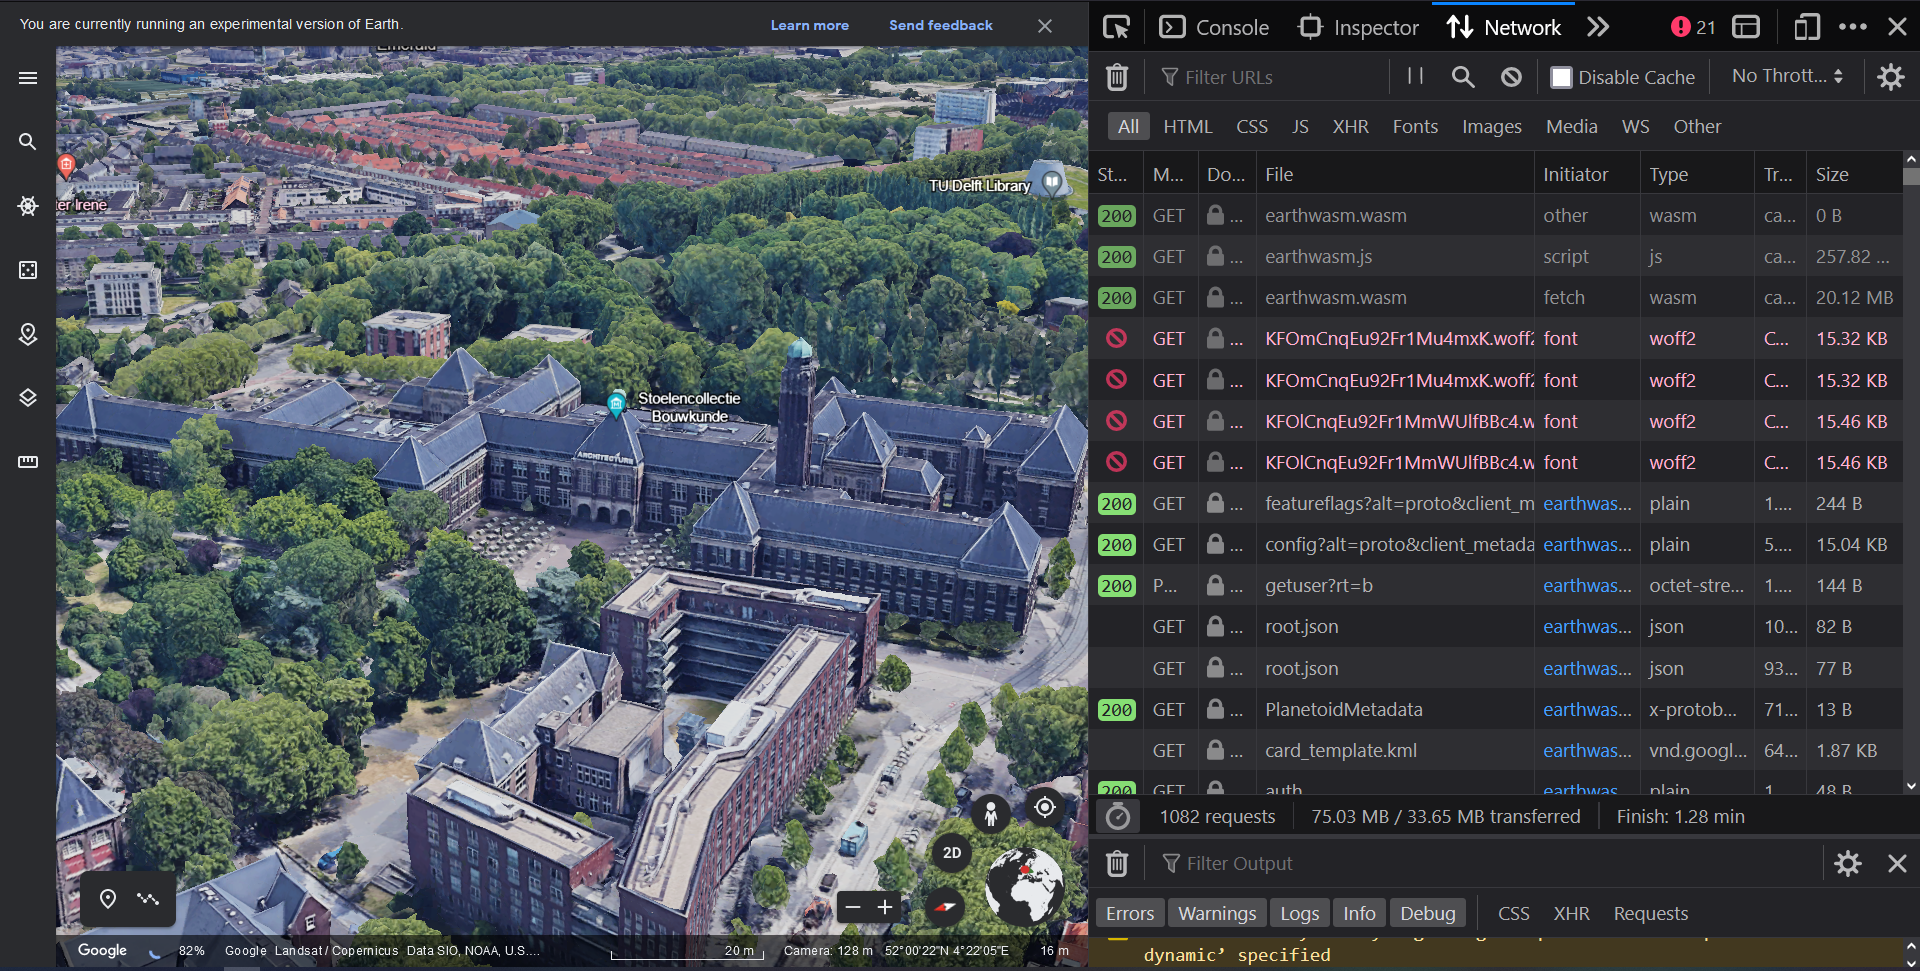
\includegraphics[width=\textwidth]{../images/google-earth-uses-webassembly.PNG}
%     \caption{Google Earth utilizing WebAssembly. Source: \cite{google_google_2020}}
%     \label{fig:google-earth}
%   \end{minipage}
% \end{figure}


% On the topic of WebAssembly, the most important conclusion to to take away from prior research is \ac{wasm} must not be regarded as a 'drop-in replacement', as \cite{melch_performance_2019} puts it. Just like any language, WebAssembly has strengths and weaknesses. While \ac{wasm} is designed to be as unassumptious and unopinionated about its source language as possible, the implementations of host environments do favor certain programming patterns and data structures over others, and this will have to be taken into account during the study.

%%%%%%%%%%%%%%%%%%%%%%%%%%%%%%%%%%%%%%%%%%%%%%%%%%%%%%%%%%%%%%%%%%%%%%%%%%%%%%%

% Based on the studies on WebAssembly, we can conclude that the compilation peculiarities of WebAssembly have to be taken into account, as it cannot be regarded as a 'drop in replacement'. There is also a significant difference between using WebAssembly theoretically, and using it realistically. The studies on Client-side geoprocessing tell us that these implementation details can have vast consequences on user experience, and studies on the Geoweb express that this user experience is vital to FAIR, cross-community geoprocessing.

% What this means for the methodology, is that a significant portion of this study's attention will have to go to experimenting with different ways of compiling to WebAssembly, while making sure it can still be used in a realistic scenario.
% If it turns out that the use-case app can only be used by experienced end-users who take special \ac{wasm} considerations in mind, a big reason of using the web, namely its accessibility, would be lost.  


%%%%%%%%%%%%%%%%%%%%%%%%%%%%%%%%%%%%%%%%%%%%%%%%%%%%%%%%%%%%%%%%%%%%%%%%%%%%%%%
% \subsubsection{(More on webassembly)}

% Not just open source: process sharing using fully containerized instances. Think .

% current vision / direction: containerized, sharable processes, together with web-based, front end visual programming environments ( RasterFoundry). Docker is usually named as a vision for these sharable processes.

% \m{->} We do have examples of cloud-native geodata formats, and some examples of cloud-based geo-computation (RasterFoundry , Google Earth Engine, more). However, these approaches have not yet tried to use truly sharable, containerized geoprocesses using Docker or WebAssembly. 

% \m{->} WebAssembly as a whole is underresearched. WebAssembly is not a fully virtualized container image, but just a binary set of instructions, meant to be executed on a virtual machine. Think of safe, cross-platform dll's. 
% WebAssembly is in this regard more simple than docker, but this gives it more opportunities. 
% WebAssembly runs in the browser for instance. 

% \m{->} This opportunity to run in the browser would enable these cloud-native frontend environments to "dry-run" these processes from within the browser, completely detached from the server, as a means to experiment with processes on a small scale before applying them to a cloud native environment. 

% \m{->} However, no implementations exist yet which combines containerized processes with these frontend computation environments. 

% # 2. BACKGROUND

% ## 2.1 The Web Browser & JavaScript
% -  main players (chrome, safari, firefox, edge(==chrome))
% - The browser js speed armsrace
% - How that lead to WebAssembly

% ## 2.2 The Geospatial Web. 
% [Still relevant]

% 2 biggest reasons against client-side geoprocessing: 
% - not performant enough
% - no equivalent to industry-standard libraries (CGAL / GDAL). 

% WebAssembly COULD solve both, so this study includes WebAssembly as 


% <br><br>

% .....

\subsection{Conclusion}
\label{sec:background-web-conclusion}

When reading \refsec{sec:background-web-terminology}, \refsec{sec:background-web-rich}, and \refsec{sec:background-wasm} together, a pattern emerges. 
WebAssembly blurs the line between the web-based and native development even further than the rich clients, and invites a further re-examination of our established models of distributed systems.
The compile target allows web-apps to make use of native libraries, and allows native software to be run on the web.
This second aspect offers a complete reverse workflow compared to the now popular Electron based applications described in \refsec{sec:background-web-rich}.
 
There was a significant initial delay between the improvements of the browser, and the widespread popularity of rich web clients. 
This study argues that as of right now, we are in the middle of a similar situation. 
A new technologies exist, it is implemented by all major browsers, and offers completely new ways of working with the web platform as a whole. 
The question remains what this will mean for the established models of clients and servers, the frontend and backend, and the web and native contexts. 

\newpage

\section{Visual Programmming}
\label{sec:background-vpl}

The third body of work this study draws from is works on the topic of visual programming. 
This section offers a brief overview on the topic itself, after which since \refsec{sec:related-geovpl} and \refsec{sec:related-webvpl} cover uses of visual programming in geocomputation and on the web, respectively. 

\subsection*{Visual programming languages}

A \ac{vpl}, or visual programming environment, is a type of programming language represented in a graphical, non-textual manner.
A VPL often refers to both the language and the \ac{ide} which presents this language in an editable way, by means of a \ac{gui}.
A visual programming language allows users to create programs by adding preconfigured components to a canvas, and connecting these components to form programs. 

Multiple types of \ac{vpl}s exist, but also multiple taxonomies of these types.
This study bases itself on the classifications presented in \cite{kuhail_characterizing_2021}, stating four different types of visual programming languages: 
\begin{enumerate}
  \item \textbf{Block-based languages}, in which all normal programming language features, like brackets, are represented by specific blocks which can be 'snapped' together (\label{fig:sidebyside:1}).
  \item \textbf{Diagram-based languages}, in which programming function are represented by nodes, and variables are represented by edges between these components (\label{fig:sidebyside:2}). This makes the entire program analogous to a Graph.
  \item \textbf{Form-based languages}, in which the functioning of a program can be configured by means of normal graphical forms (\label{fig:sidebyside:3}). 
  This approach enhances the stability and predictiveness compared to other types, at the cost of expressiveness.
  \item \textbf{Icon-based languages}, in which users are asked to define their programs by chaining highly abstract, iconified procedures (\label{fig:sidebyside:4}). 
\end{enumerate}

The meta analysis of \cite{kuhail_characterizing_2021} shows a great preference among researchers for block- and diagram-based languages. 
Only 4 out of 30 of the analyzed articles chose a form-based vpl, and only 2 chose an icon-based approach.  

This study wishes introduce a fifth type of VPL. 
A \textbf{Dataflow} VPL is a subtype of a diagram based VPL which only uses pure functions as computation nodes, only uses immutable variables, and which disallows cyclical patterns. This makes this VPL not only a graph, but a \ac{dag}.
More on this in \refsec{sec:background:dataflow}.

\begin{figure}
\centering
\begin{subfigure}[b]{0.45\linewidth}
  \graphicspath{{../../assets/images/background/vpl/}}
  \centering
  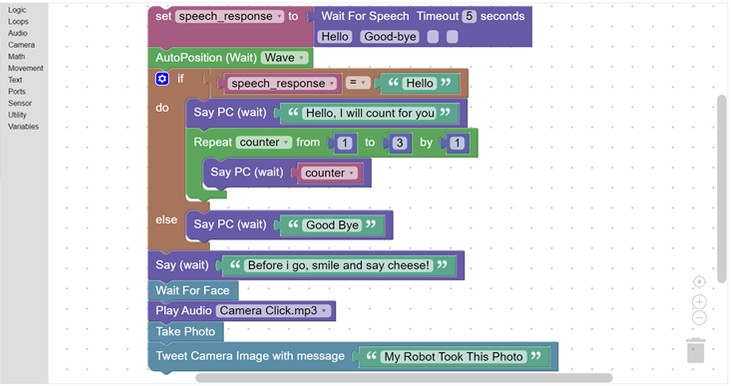
\includegraphics[width=\linewidth]{block-based.png}
  \caption{}\label{fig:vpl-types:1}
\end{subfigure}%
\qquad %-- that adds some space between th 2 figures
\begin{subfigure}[b]{0.45\linewidth}
  \graphicspath{{../../assets/images/background/vpl/}}
  \centering
  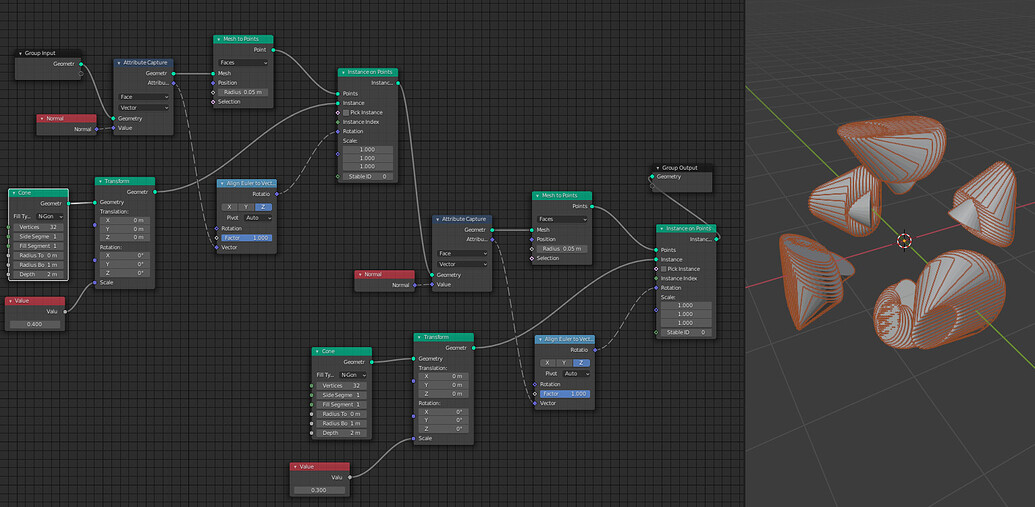
\includegraphics[width=\linewidth]{diagram-based.jpg}
  \caption{}\label{fig:vpl-types:2}
\end{subfigure}%
\\
\begin{subfigure}[c]{0.45\linewidth}
  \centering
  \graphicspath{{../../assets/images/background/vpl/}}
  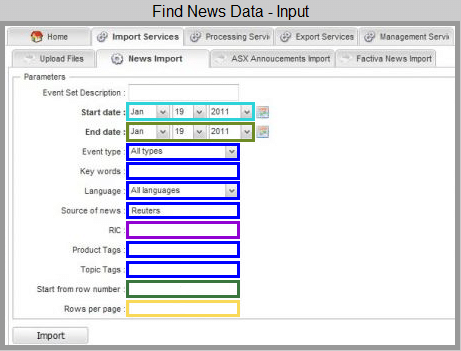
\includegraphics[width=\linewidth]{form-based.png}
  \caption{}\label{fig:vpl-types:3}
\end{subfigure}%
\qquad %-- that adds some space between th 2 figures
\begin{subfigure}[d]{0.45\linewidth}
  \centering
  \graphicspath{{../../assets/images/background/vpl/}}
  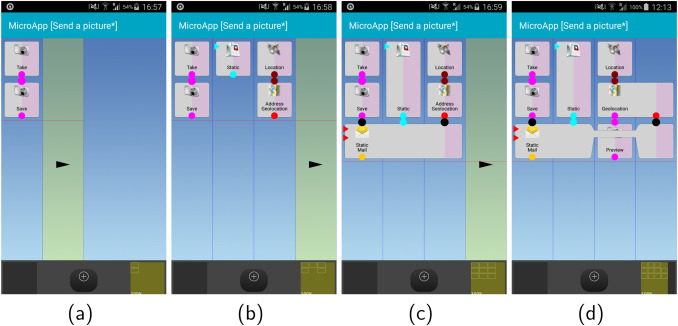
\includegraphics[width=\linewidth]{icon-based.jpg}
  \caption{}\label{fig:vpl-types:4}
\end{subfigure}%
\caption[Types of \ac{vpl}s]{Four different types of visual programming languages: Block-based, diagram-based, form-based, and icon-based, respectively}%
\label{fig:vpl-types}
\end{figure}

Visual programming languages are used in numerous domains. 
The vpls of the 30 studies examined by (SOURCE) were aimed at domains such as the Internet of Things, robotics, mobile application development, and augmented reality. 
Within the domain of systems control and engineering, The Ladder Diagram vpl (SOURCE) is the industry-standard for programming Programmable Logic Controllers (PLCs).
\ac{vpl}s are also widely used within computer graphics related applications, including the field of \ac{gis}, 
These will be covered in \refsec{sec:related-geovpl}.
Lastly, \ac{vpl}s also have great educational applications. 
Harvard's introduction to computer science course, CS50, famously starts out with Scratch, a block-based visual programming language normally targeted at children, to teach the basics of computational thinking (Source: CS50). 

% \begin{note}
%   Traditionally, visual programming has been successfully used to help novices
%   learn basics of programming by visualizing elements of a program. 
%  However, visual programming is increasingly being used by end 
%  users in various domains to create and tailor applications that are useful 
%  beyond the realm of education. 
%  For instance, VPLs are now being used in fields such as 
%  the 
%  From characterizing_2021
 

\subsection{Usability}

Studies on \ac{vpl}s indicate that generally speaking, VPLs make it easy for end users to visualize the logic of a program, and that vpls eliminate the burden of handling syntactical errors \cite{kuhail_characterizing_2021}.

The locally famous Cognitive Dimentions study \cite{green_usability_1996}, states that \emph{"The construction of programs is probably easier in VPLs than in textual languages, for several reasons: 
there are fewer syntactic planning goals to be met, such as paired delimiters, discontinuous constructs, separators, or initializations of variables; 
higher-level operators reduce the need for awkward combinations of primitives; 
and the order of activity is freer, so that programmers can proceed as seems best in putting the pieces of a program together."}. 
Indeed, a vpl UI can be used to eliminate whole classes of errors on a UI level by, for example, not allowing the connection of two incompatible data types. 

\begin{note}
  TODO: this is a weak argument. This also needs to be more nuanced
\end{note}

% //The meta analysis of \cite{kuhail_characterizing_2021} also 

These properties together make visual programming also highly suitable for activities of \textbf{experimentation} and \textbf{debugability}, and not only for end users. 

% ADVANTAGE: PLAYFULNESS

\subsection{End User Development \& Low Coding}
a \ac{vpl} done right can make automation available to a very large audience, and this is exactly the point. 
Visual Programming is part of a larger field, named End User Development (eud). 
The field is concerned with allowing end users who are not professional software developers to write software applications, using specialized tools and activities. 
This however, does not mean that experienced developers have nothing to gain from this research. 
Lowering the cognitive load of certain types of software development could save time and energy which can then be spend on more worthwhile and demanding tasks. 

\cite{kuhail_characterizing_2021} point out two serious advantages of EUD. 
First, end users know their own domain and needs better than anyone else, and are often aware of specificities in their respective contexts (\cite{kuhail_characterizing_2021}). 
And two, end users outnumber developers with formal training at least by a factor of 30-to-1 according to Kuhail et. al., and my suspicion is that this might be much higher.

% rewrite this more professionally...
I would like to add that offering the general public a chance to automate repetitious workflows might not only increase productivity, but can also greatly improve the quality of life in general, by focussing on the profound instead of the mundane. 

In the private sector, \ac{eud} is represented by the "low code" industry. 
Technology firms such as Google and Amazon are investing at scale in low-coding platforms (\cite{kuhail_characterizing_2021}),
The market value was estimated at 12.500 Million USD (Source: ), and with a growth rate between 20 and 40 percent, the value may reach as high as 19 Billion by 2030 (SOURCE: FORRESTER) 

\subsection{Dataflow programming}
\label{sec:background:dataflow}
An important aspect of the dataflow-VPL is the connection to the field of dataflow programming, which is not necessarily linked to VPLs. 

Dataflow programming is a programming paradigm which internally, represents a program as a \ac{dag} (SOURCE Dataflow 2012). 
A graphical, editable representation of a dataflow program would result into a Dataflow \ac{vpl}.

The big computational advantage of this model, is that it allows for implicit concurrently (SOURCE dataflow 2012). 
In other words, every node of a program written using dataflow programming can be executed in isolation of any other nodes, as long as the direct dependencies (the inputs) are met. 
No global state or hidden side effects means no data-race issues, which allows parallel execution of the program by default.
When using other paradigms, programmers need to manually spawn and manage threads to achieve the same effect. 

This leads into an interesting side-effect of using dataflow programming / a diagram-based \ac{vpl}: 
By only permitting pure, stateless functions with no side-effect, and only immutable variables, end users automatically adopt a functional programming style (albeit without lambda functions).
Functional programming has many benefits of its own besides concurrency, such as clear unit testing, hot code deployment, debugging advantages, and lending itself well for compile time optimizations (SOURCE: functional programming).


% functional programming

% Spreadsheets are probably the most common example of DFP
% and widely adopted by every type of computer users.
% On a spreadsheet, each cell represents a node that can either be an expression
% or a single value. Dependencies can exist to other cells. Following the dataflow
% model, whenever a cell gets updated, it sends its new value to those who depend
% on it, that update themselves before also propagating their new values. This
% specific type of application is commonly denominated as Cell-Oriented DPF or
% Reactive programming.

The important take-away is this: 
A \ac{vpl} is not just a matter of a user-friendly UI or a stylistic choice.
This might be true for block-based vpls, but not for diagram-based vpls. 
By closely resembling dataflow itself, and because of its functional programming nature, diagram-based vpls can actually lead to faster and more reliable software.

\subsection{Disadvantages and open problems}
\label{sec:background:vpl:disadvantages}

there is of course, no such thing as a free lunch. 
\ac{vpl}s and dataflow programming en large have got certain disadvantages and open problems.

% (Dataflow programming is an area still open to further research, with some open
% issues to answer. In fact, most of the open questions today have long been
% identified and despite the improvements, patterns for answering them are yet to
% be achieved.)

% block-based visual programming: just purely UI, diagram-based vpl add additional, functional programming qualities. 


\subsubsection*{Iteration and conditionals}

\begin{figure}
  \centering
  \begin{subfigure}[b]{0.45\linewidth}
    \graphicspath{{../../assets/images/background/vpl/}}
    \centering
    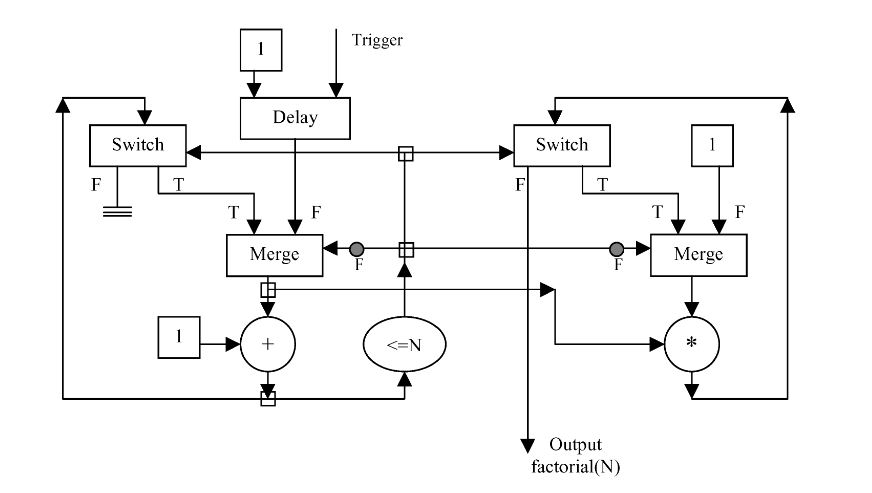
\includegraphics[width=\linewidth]{iteration-vpl.png}
    \caption{}\label{fig:vpl-iteration:1}
  \end{subfigure}%
  \qquad %-- that adds some space between th 2 figures
  \begin{subfigure}[b]{0.45\linewidth}
    \graphicspath{{../../assets/images/background/vpl/}}
    \centering
    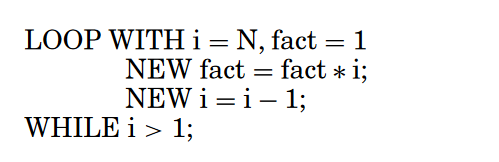
\includegraphics[width=\linewidth]{iteration-text.png}
    \caption{}\label{fig:vpl-iteration:2}
  \end{subfigure}%
  \caption[Comparrison of iteration]{A factorial function, written in a vpl, and textual form}%
  \label{fig:vpl-iteration}
  \end{figure}

A problem described in almost all reviewed vpl literature (Source: advanced in dataflow, SOURCE: Dataflow programming,  SOURCE: COGNITIVE), is that the \ac{dag} model of diagram-based vpls are ill-suited for representing even the most basic flow control statements: \m{if, else, for, while}.
Even if the acyclic quality of the dataflow graph is omitted, the resulting models are significantly more complicated compared to their textual counterparts, as shown by \reffig{fig:vpl-iteration}.

\subsubsection*{Encapsulation \& reusability}
Similar and yet different is the topic of encapsulation, or, how (SOURCE: COGNITIVE) names this problem: 'visibility'.
It is widely known that as a program scales in size, the complexity of handling the application scales exponentially.
In textual languages, reducing this complexity is often achieved by means of encapsulating sub-routines and re-usable parts of the program into separate functions.
Inner functionality is then hidden, and operations can be performed on a higher level of abstraction. 
This hierarchy of abstraction is just as achievable for \ac{vpl}s as described by (SOURCE: Dataflow programming).
However only a select number of \ac{vpl}s offer a form of encapsulation, and even less allow the creation of reusable functions, or creating reusable libraries from vpl scripts.
It appears that \ac{vpl} researches and developers are either not aware of the importance of encapsulation, or have encountered problems in representing this feature in a graphical manner.

% \subsubsection{High viscocsity}
% Viscosity was surprisingly high in the languages we looked at. The role of the diagram editor is crucial, yet few research papers in the usual programming literature discuss the design of effective diagram editors. In our straw viscosity test we found a range from about 1 minute to about 9 minutes for making semantically equivalent changes to programs in different languages. Visibility can be very poor. Systematic, easy-to-understand search tools need to be developed and user-tested, and if at all possible de facto standards should be adopted.

\subsubsection*{Subjective Assessment}
Additionally, the claims that \ac{vpl}s lend themselves well for end-user development is problematic from a technical perspective. 
Usability is a nebulous phenomenon, and challenging to measure empirically.
As often with more subjective matter, researchers have yet to form a consensus over a general evaluation framework. 
There is, however, a reasonable consensus on the 'qualities' a VPL should aspire to. 
This is different from a full assessment framework, but nontheless useful for comparing \ac{vpl}s.
The dimensions given in the cognitive dimensions framework (SOURCE) have acquired a somewhat canonical nature within \ac{vpl} research.
The number of citations of this work is relatively high, and indeed, almost all \ac{vpl} studies the author was able to find referred back to this critical work.   
In so far as this study needs to address the usability of the prototype VPL, we will thus follow this consensus, and base any assessment on (SOURCE).

% - we will make no such attempt. usability serves as background motivation. 
% - this study assumes vpl's are 'in general' more usable to end-users 
% than text-based alternatives, based on the positive results of most of the 
% studies analysed by communicating_2021.

\subsubsection*{Lacking Life-cycle support}
Finally, (communicating 2021) names the 'life cycle' of applications created by \ac{vpl}s as one of the most overlooked aspects within VPL research.
Out of the 30 studies covered by the meta analysis, only one briefly touched the topic of life cycle. 
Life cycle in this context refers to all other activities besides "creating an application that does what it needs to do".
Examples of these activities are version control, extending an existing application, debugging, testing the codebase, and publishing the application to be used outside of an \ac{ide}. 
These operational aspects are critical to making any application succeed, and \ac{eud} research should not be limited to purely the aspect of creating functionalities.

This oversight on life-cycle aspects can be found in the \ac{vpl} \& low-coding industry as well. 
\begin{note}
TODO: Formalize these ramblings, or don't. 

- no existing VPL ( that I know of ) has proper git-based version control. 
  - Most vpls use proprietary storage and collaboration methods. 
- vpls which are able to compile to a textual format are rare
  - vpls able to compile to a programming language, or a headless format, are even more rare. 

- Let alone: on operational programming paradigms such as Test driven development (TDD), continuous integration (CI), continuous delivery (CD).  

- in general, the life-cycle support of most vpls found in the low-coding industry are closely tied to their business models. 
  - Users can only use the publication tools, version control tools, and package / library managers offered to them by the vendor.

\end{note}

And while we are on the topic of publication, only 16 out of 30 of the tools analysed by (communicating 2021) were available publicly with some documentation.
It seems the lack of publication tooling might also partially be due to a lack of publication in general. 

\subsection{Conclusion}

The background literature clearly indicates many advantageous properties of vpls, both in terms of (end) user experience and the dataflow programming properties. 
Additionally, the studies showed important considerations which have to be taken into account in the design of any vpl.  
Lastly, the studies agree on several open-ended issues of which a satisfying answer is yet to be found. 

%%%%%%%%%%%%%%%%%%%%%%%%%%%%%%%%%%%%%%%%%%%%%%%%%%%%%%%%%%%%%%%%%%%%%%%%%%%%%%%
%%%%%%%%%%%%%%%%%%%%%%%%%%%%%%%%%%%%%%%%%%%%%%%%%%%%%%%%%%%%%%%%%%%%%%%%%%%%%%%
%%%%%%%%%%%%%%%%%%%%%%%%%%%%%%%%%%%%%%%%%%%%%%%%%%%%%%%%%%%%%%%%%%%%%%%%%%%%%%%

\chapter{Related works}
\label{chap:related}

This chapter offers a review of related and comparable studies and projects.
While almost no studies exist at the intersection of all three of these fields, we do find many related studies and projects which intersect two of these fields, represented by the edges of \reffig{fig:triangle-model}:
\begin{enumerate}[-]
  \item \refsec{sec:related-geoweb} reviews related works on browser-based geoprocessing
  \item \refsec{sec:related-geovpl} reviews related works on VPLs used for geo-computation
  \item \refsec{sec:related-webvpl} reviews related works on VPL web applications
\end{enumerate}

\begin{figure}
  \centering
  \graphicspath{ {../../assets/diagrams/} }
  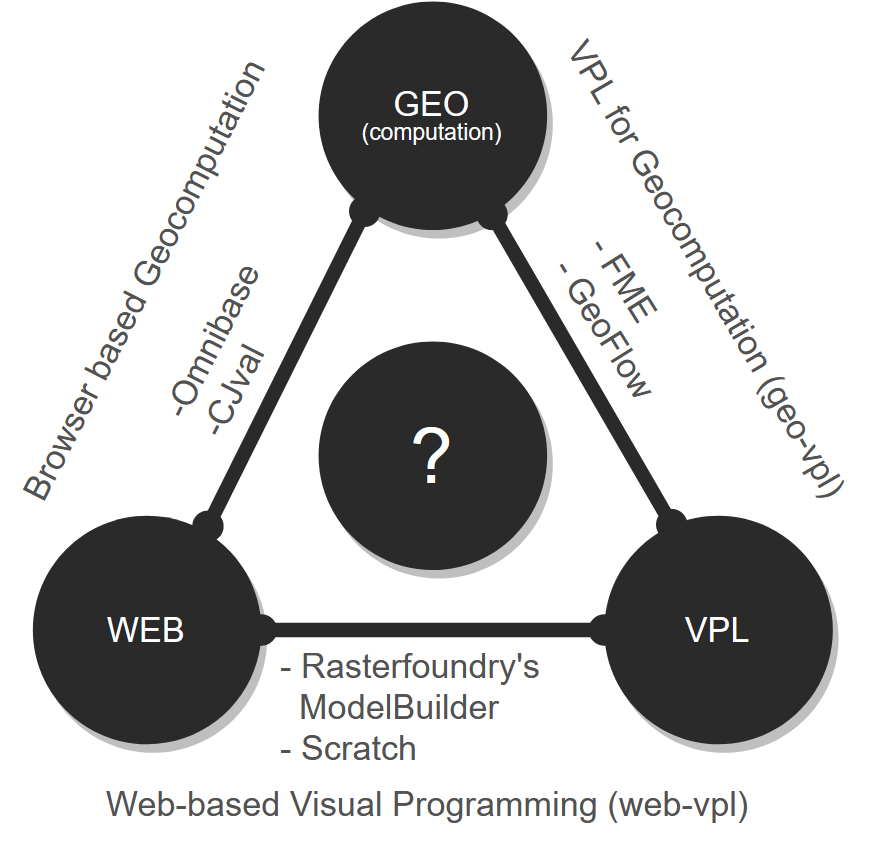
\includegraphics[width=270px]{geo-web-vpl.png}
  \caption{Triangle Model}
  \label{fig:triangle-model}
\end{figure}

\section{Browser-based geocomputation}
\label{sec:related-geoweb}

This section is dedicated to related works on client-side geocomputation, or browser-based geocomputation. 
this study prefers to use "browser-based geocomputation" in order to circumvent the ambiguity between native clients like QGIS \cite{qgis_community_qgis_2022}, and web clients like omnibase.

% First, a small paragraph on the motivation behind browser based geocomputation.
% As stated in \refsec{sec:background-web}, web applications offer safety, distribution and accessibility advantages over native applications.
% As such, browser based \ac{GIS} has become a sizable component of the full geospatial software landscape. 

% % For the average person, an interactive \ac{gis} web application is often their first and only exposure to such a system, be it a web mapping service, a navigation system, or a pandemic outbreak dashboard. 
% However, despite the popularity of geographical web applications, the range of actual \ac{GIS} abilities these applications have is generally speaking very limited. 
% \ac{geocomputation} is usually not present within the same software environment as the web app. 
% This limited range of capabilities inhibits the number of use cases geographical web applications can serve, and with that the usefulness of web \ac{GIS} as a whole.
% If web applications gain \ac{geocomputation} capabilities, they could grow to be just as diverse and useful as desktop \ac{gis} applications, with the added benefits of being a web application. It would allow for a new range of highly accessible and sharable geocomputation and analysis tools, which end-users could use to post-process and analyze geodata quickly, uniquely, and on demand.

Browser-based geocomputation has seen some academic interest throughout the last decade \cite{hamilton_client-side_2014, panidi_hybrid_2015, kulawiak_analysis_2019}.
Interactive geospatial data manipulation and online geospatial data processing techniques have been described as "current highly valuable trends in evolution of the Web mapping and Web GIS" \cite{panidi_hybrid_2015}. 
The central idea is to add browser-based geocomputation to web-mapping applications, allowing users not only to view geodata, but to analyze it, and even fine-tune the data to their own custom needs.
An example of this is the Omnibase application \citep{geodelta_omnibase_2022} in \reffig{fig:1:omnibase}, used by Dutch municipalities to measure buildings and infrastructure based on point clouds and oblique multi-stereo imagery.

\begin{figure}
  \centering
  \graphicspath{ {../../assets/images/background/geo-web/} }
  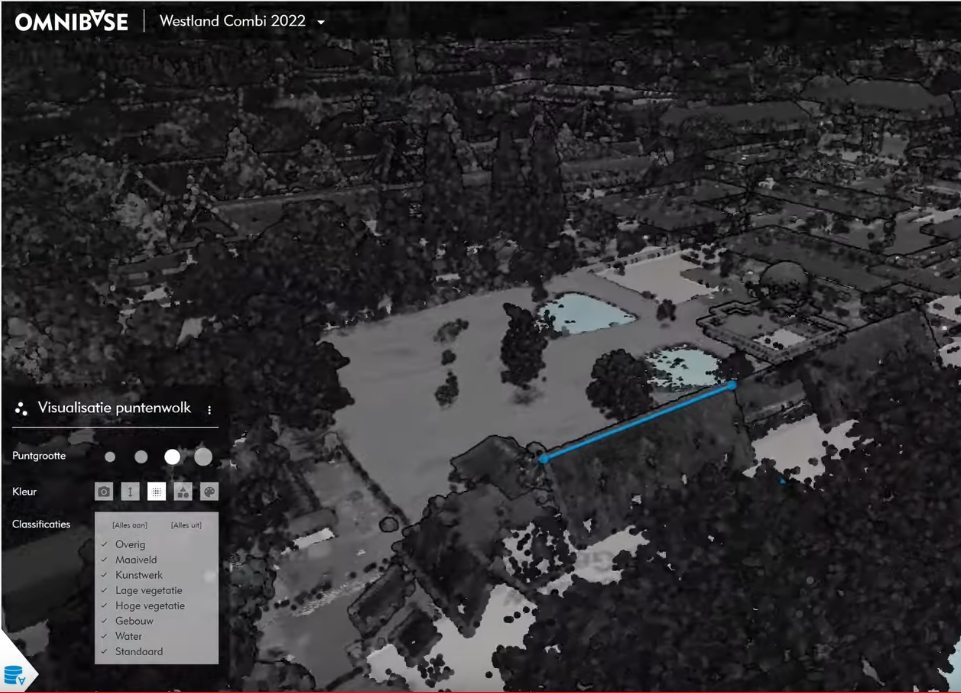
\includegraphics[width=250px]{omnibase.png}
  \caption{Omnibase: An example of browser-based geocomputation \citep{geodelta_omnibase_2022}}
  \label{fig:1:omnibase}
\end{figure}

browser-based geocomputation, compared to native GUI or CLI geocomputation, allows geocomputation to be more accessible and distributable. 
Accessible, since geocomputation on the web requires no installation or configuration, 
and distributable, since the web is cross-platform by default, and poses many advantages for updating, sharing, and licensing applications. 
Lastly, by performing these calculations in the browser rather than on a server, server resources can be spared, 
and customly computed geodata does not have to be resent to the user upon every computation request.

However, browser-based geocomputation poses multiple challenges. 
The big catch is that browsers \& javascript are not ideal hosts for geocomputation. 
As an interpreted language, Javascript is slower and more imprecise compared to system-level languages like C++.
In addition, it has limited support regarding reading and writing files, and does not possess of a rich ecosystem of geocomputation libraries.  
Novel browser features like WebAssembly may pose a solution to some of these open questions, but this has not seen substantial research. 

\subsection{Examples}

\citet{hamilton_client-side_2014} created a 'thick-client', capable of replacing certain elements of server-side geoprocessing with browser-based geoprocessing. 
The results of this study were unfavorable. 
The paper states how "the current implementation of web browsers are limited in their ability to execute JavaScript geoprocessing and not yet prepared to process data sizes larger than about 7,000 to 10,000 vertices before either prompting an unresponsive script warning in the browser or potentially losing the interest of the user." \citep{hamilton_client-side_2014}. 
While these findings are insightful, they are not directly applicable to the efforts of this study proposal. Three reasons for this:

\begin{itemize}
  \item The paper stems from 2014. Since then, web browsers have seen a significant increase in performance thanks to advancements in JavaScript JIT compilers \citep{haas_bringing_2017, kulawiak_analysis_2019}. 
  \item The paper does not utilize compile-time optimizations. The authors could have utilized 'asm.js' \citep{mozilla_asmjs_2013} which did exist at the time. 
  \item The paper uses a javascript library which was never designed to handle large datasets.
\end{itemize}

The same statements can be made about similar efforts of \citet{panidi_hybrid_2015}. 
However, Panidi et. al. never proposed browser-based geoprocessing as a replacement of server-side geoprocessing. 
Instead, the authors propose a hybrid approach, combining the advantages of server-side and browser-based geoprocessing. 
They also present the observation that browser-based versus server-side geoprocessing shouldn't necessarily be a compassion of performance. 
"User convenience" as they put it, might dictate the usage of browser-based geoprocessing in certain situations, despite speed considerations \cite{panidi_hybrid_2015}. 

This concern the general web community would label as \ac{UX}, is shared by a more recent paper \cite{kulawiak_analysis_2019}. 
Their article examines the current state of the web from the point of view of developing cost-effective Web-GIS applications for companies and institutions. 
Their research reaches a conclusion favorable towards browser-based data processing: "[Client-side data processing], in particular, shows new opportunities for cost optimization of Web-GIS development and deployment. 
The introduction of HTML5 has permitted for construction of platform-independent thick clients which offer data processing performance which under the right circumstances may be close to that of server-side solutions. 
In this context, institutions [...] should consider implementing Web-GIS with client-side data processing, which could result in cost savings without negative impacts on the user experience.".

% Based on the topic of client-side geospatial processing, we can state that web technologies contain a very dynamic temporal component. All research can become outdated, but performance analysis of web technologies are especially quick to change.  

From these papers we can summarize a true academic and even commercial interest \\ in browser based geoprocessing over the last decade. 
However, practical implementation details remain highly experimental, or are simply not covered.  
The implementations of \cite{panidi_hybrid_2015, hamilton_client-side_2014} were written in a time before WebAssembly \& major javascript optimizations, and the study of \cite{kulawiak_analysis_2019} prioritized theory over practice. 
Additionally, to the best of the authors's knowledge, all papers concerned with browser-based geoprocessing either tried to use existing JavaScript libraries, or tried to write their own experimental WebAssembly / JavaScript libraries. 
No studies have been performed on the topic of compiling existing C++/Rust geoprocessing libraries to the web. 

%%%%%%%%%%%%%%%%%%%%%%%%%%%%%%%%%%%%%%%%%%%%%%%%%%%%%%%%%%%%%%%%%%%%%%%%%%%%%%%
\subsection{Commercial web-based geocomputations software}

Despite the earlier statement of the general lack of \ac{geocomputation} within browsers, there are exceptions. 
A select number of web-based \ac{GIS} applications are starting to experiment with empowering end-users with geocomputation. 
These applications will briefly be mentioned.
 
% https://geotiff.io/
GeoTIFF (\citep{dufour_geotiffio_2022}, \reffig{fig:geotiff}), is a web-based, open source, geoTIFF processing tool. 
It offers basic operations such as taking the median or \& mean of a certain area, color band arithmetic, and can plot histograms, all calculated within the browser using customly written javascript libraries.

\begin{figure}
  \centering
  \graphicspath{ {../../assets/images/background/geo-web/} }
  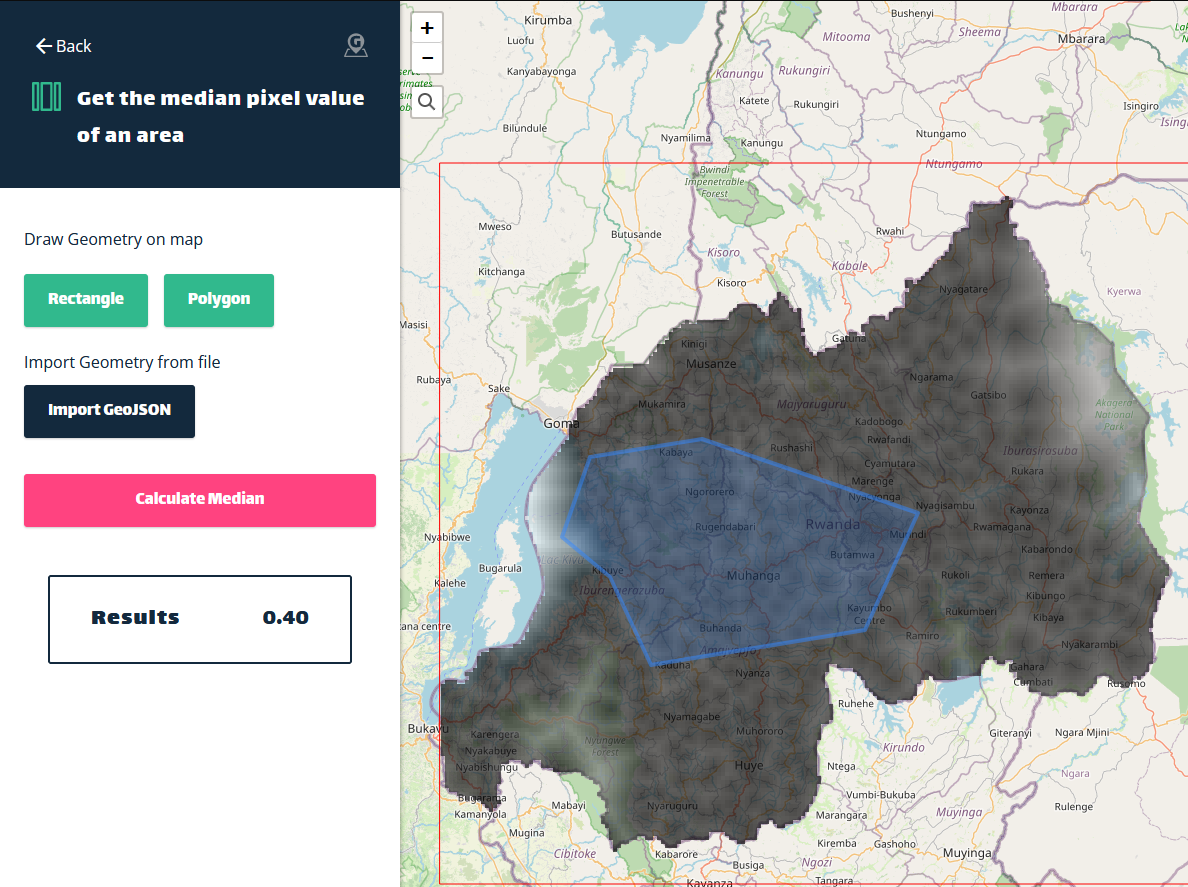
\includegraphics[width=270px]{geotiff.png}
  \caption{The geoTIFF.io application \citep{dufour_geotiffio_2022}}
  \label{fig:geotiff}
\end{figure}

\begin{figure}
  \centering
  \graphicspath{ {../../assets/images/background/geo-web/} }
  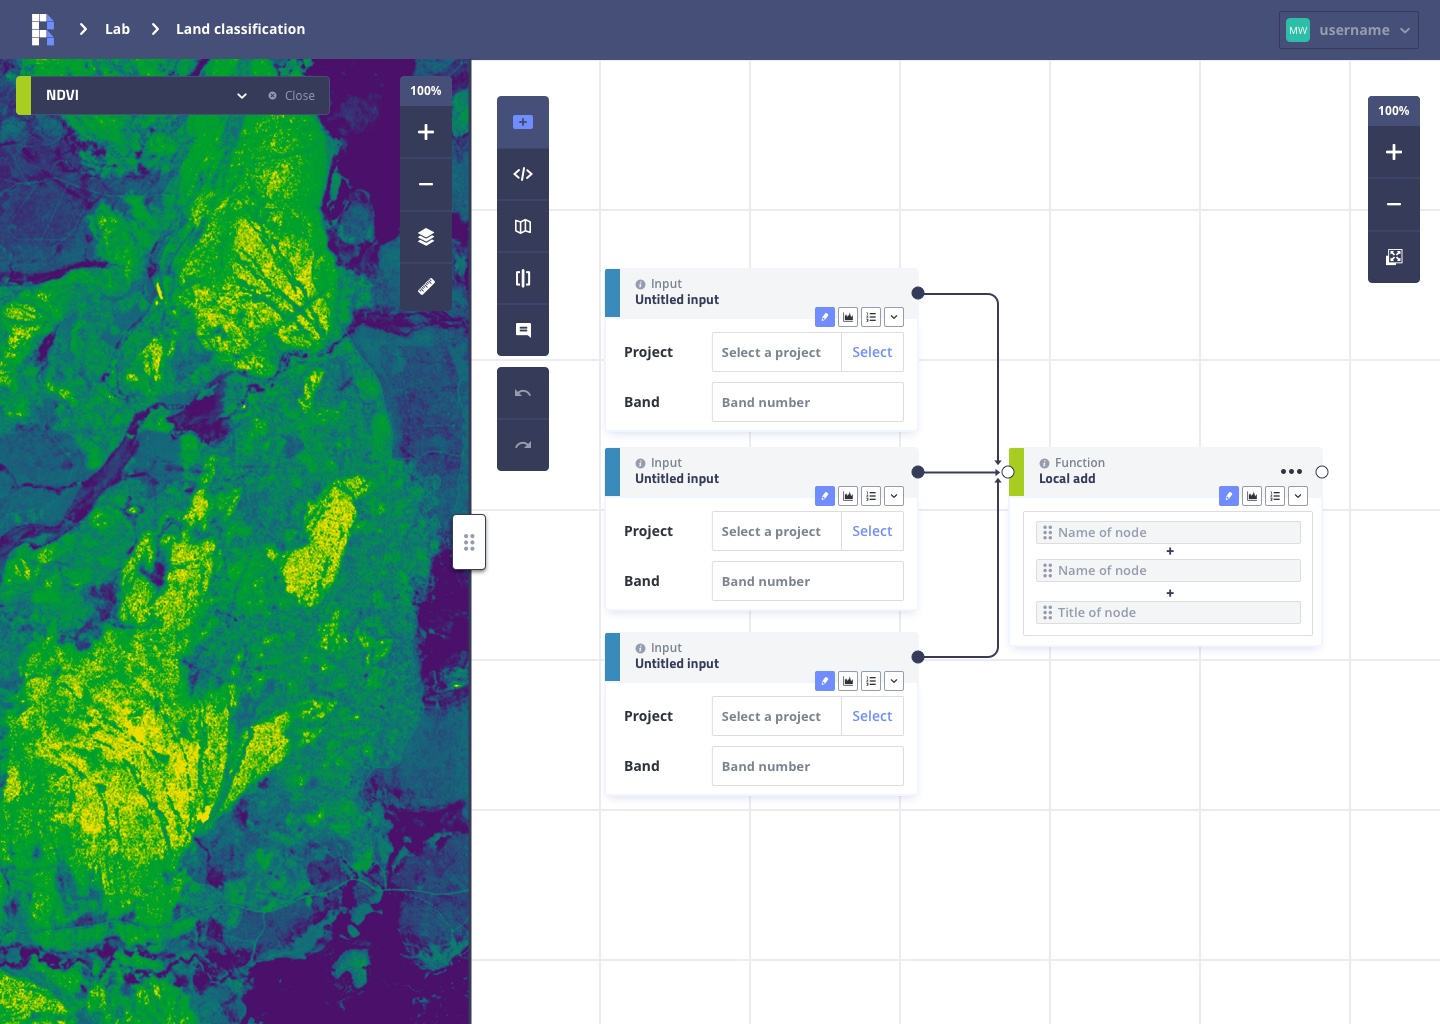
\includegraphics[width=270px]{rasterfoundry-2.jpg}
  \caption{The ModelLab application \citep{azavea_geotrellis_2022}}
  \label{fig:modellab}
\end{figure}

The modelLab application by Azavea, is also a GeoTIFF / raster based web processing tool, in which basic queries and calculations are possible \citep{azavea_geotrellis_2022}. 
This tool offers more advanced types of geocomputation, like buffering / minkowski sums, and even multi-stage processing via a simple but clear visual programming language (see \reffig{fig:modellab}). 
% There reasoning: "Widespread access to frequent, high-resolution Earth observation imagery has created the need for innovative tools like ModelLab that will 
However, the tool uses mostly server-side processing, making this application less relevant to this study. 

% Also, despite their mission statement to: "help individuals and organizations to effectively access, analyze, edit, and visualize remotely sensed data in transformative new ways without years of specialized training or ongoing investments in proprietary software and technology infrastructure."(Source), The tool appears to be reliant on their own proprietary infrastructure to save and run the application.
% The author of this study was also not able to find a public demo of the application. 

\begin{figure}
  \centering
  \graphicspath{ {../../assets/images/background/geo-web/} }
  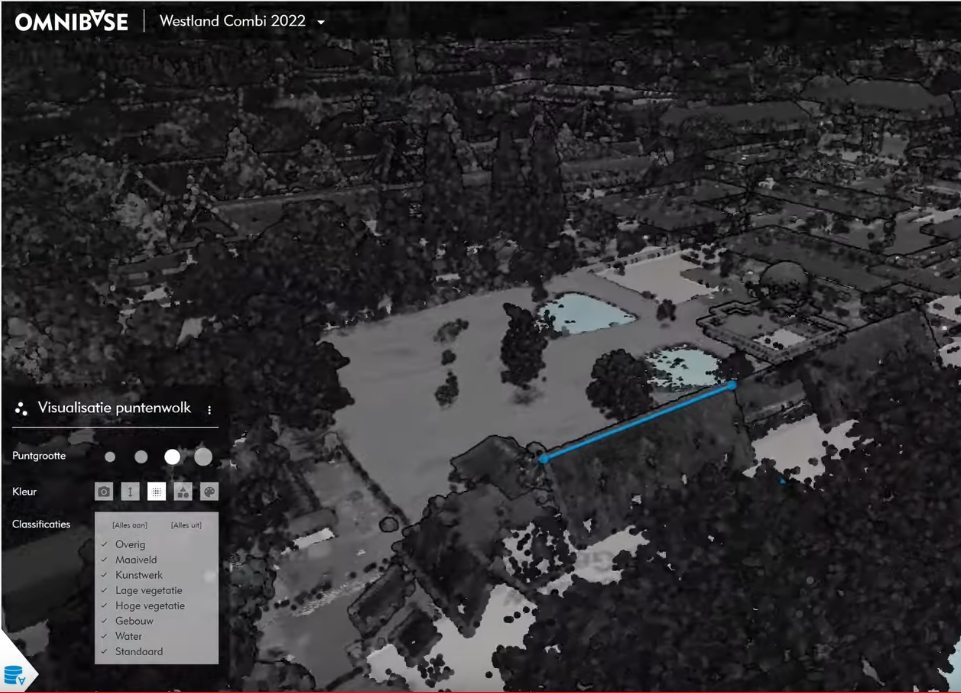
\includegraphics[width=270px]{omnibase.png}
  \caption{The Omnibase application \citep{geodelta_omnibase_2022}}
  \label{fig:omnibase}
\end{figure}

The last web-based geocomputation platform this study would like to mention is Geodelta's Omnibase application \citep{geodelta_omnibase_2022} (see \reffig{fig:omnibase}). 
Omnibase is a 3D web \ac{GIS} application for viewing and analyzing pointclouds and oblique multi-stereo imagery.
It offers client-side geocomputation in the form of measuring distances between locations, and calculating the area of a polygon.  
It also offers photogrammetry-techniques such as forward incision of a point in multiple images, but these are calculated server-side. 

% - https://openscad.org/


%%%%%%%%%%%%%%%%%%%%%%%%%%%%%%%%%%%%%%%%%%%%%%%%%%%%%%%%%%%%%%%%%%%%%%%%%%%%%%%
%%%%%%%%%%%%%%%%%%%%%%%%%%%%%%%%%%%%%%%%%%%%%%%%%%%%%%%%%%%%%%%%%%%%%%%%%%%%%%%
%%%%%%%%%%%%%%%%%%%%%%%%%%%%%%%%%%%%%%%%%%%%%%%%%%%%%%%%%%%%%%%%%%%%%%%%%%%%%%%

%  \subsection*{The Cloud Native Geospatial movement}

% ( Not sure if I wanna go there... )

% % Establish OGC in two sentences, mentioning their name and Vision
% The Open Geospatial Consortium (OGC)...
% Mission: FAIR Geodata 

% % Establish Cloud Native movement.
% % GIS as one big LAN party
% A prominent development within the OGC is the recent effort towards a \textbf{"Cloud Native Geospatial"} future. 
% This initiative aims to radically simplify geodata storehouses to static servers serving large, singular binary geodata files. All processing and analysis of this geodata can then be performed by separate cloud-based web services. 
% This architecture has many advantages over current geodata storage and analysis methods:
% \begin{itemize}
%   \item These new Cloud Native geodata formats are much cheaper to access by front-end and back-end services, compared to active services.
%   \item Substituting active SQL or noSQL databases by static binary files is easier and cheaper for data providers, leading to more and more readily available geodata.
%   \item By using supercomputers (Microsoft Planetary Computer) and cloud-storage (AWS), Geodata processes could make use of near-infinite computational and storage resources. 
%   \item By having all data centralized in one location or type of location, new, large scale patterns within our geodata could be discovered.  
%   \item For web GIS, this would offer direct data streaming options, similar to services like "Netflix" or "Spotify".  
% \end{itemize}

% These features may have a far reaching impact on society. Chris Holmes, forerunner of the cloud-native geospatial movement, envisions what the movement could mean for even non-GIS users: 
% \emph{
%   With the introduction of accessible, centralized data, and the dramatically different workflows that follow, Cloud Native Geospatial has the potential to introduce new, non-specialized users to the power of geospatial information that GIS practitioners have enjoyed for decades. [...]. The ecosystem of geospatial experts will collaborate to create analyses and insight, but any non-expert user will be able to select and apply those to the geographic area they care about. \~ Chris Holmes
% }
% % This is also reflected by cloud-native based tools like (Google Earth Engine or RasterFoundry) may achieve such a feed, by being web based and stuff...
% All these reasons explain why the OGC and many other parties are now actively pursuing this vision.

% But while this vision is in active development, many large-scale challenges are still in its way. 
% One of the most important challenges is the required paradigm shift within geo-computation / geoprocessing workflows. 
% The current, common geo-computation workflow of retrieving online data, only to run it through a local process and send the resulting data back into servers, will have to be reversed: In a cloud-native future, we will not retrieve data for our local process, but we will upload our process to the data.  
% This introduces a sizable challenge: \textbf{Portable, Containerized Geo-computation}.

% % \textbf{and the algorithms powering the processing can be shared online and customized collaboratively}. -> Chris again

% % \begin{itemize}
% %   \item Up to this point, the world of GIS has done a considerable effort to make geodata more Findable, Accessible, Interoperable, and Reusable. The challenge of Portable geo-computation now forces us to extent the effort of FAIR geodata to FAIR geodata computation as well.  
% %   \item If we want our geodata processes to be just as portable as the geodata it takes as input, then perhaps the FAIR paradigm should extent from FAIR geodata to FAIR geodata processing . FAIR geo-computation.
% %   \item Furthermore, it remains a mystery how these containerized containerized processes will be configured and accessed by frontend computation environments. 
% %   \item Holmes: one of the vital ingredients: \emph{"and the algorithms powering the processing can be shared online and customized collaboratively"}.
% % \end{itemize}

% The challenge of sharing and chaining together containerized fragments of geoprocesses to a variety of environments will require more than just open source collaboration. 
% This study interprets the challenge of portable geo-computation by means of the FAIR paradigm. 
% If geodata processes need to be just as portable as the geodata forming the input and output, then perhaps the FAIR paradigm should extent from FAIR geodata to FAIR geodata \emph{processing} as well.
% The challenge facing the cloud-native vision then becomes: \textbf{How to make geo-computation Findable, Accessible, Interoperable, and Reusable?} 
% This links back to containerization, for containerization is a very powerful method of making geo-computation more Interoperable and Reusable.

% % state of the art regarding this issue, make a path towards the particular thesis, and why it is an application
% The current state of the art is far removed from either portable or FAIR geo-computation. 
% \todo{Improve this intro}
% \begin{itemize}
%   \item current methods: Docker, and some geo-computation platforms.
%   \item Not many implementations using WebAssembly, while this is a prime candidate: Even the guy who made Docker said so. 
%   \item ignore the cloud: focus on the act of containerizing geoprocesses using webassembly an sich
% \end{itemize}

\newpage
\section{Visual programming and geocomputation}
\label{sec:related-geovpl}

This section is dedicated to giving an overview of related works on \ac{VPL}s related to geocomputation.

% \begin{note}
%   [I just wish to state: "these applications exist".
%   I also wish to make some comments on the interplay between geocomputation and vpl. 
%   Are these fields complimentary?
%   These will also be referred back to during the methodology chapter]    
% \end{note}

\reffig{fig:geovpl:table} offers this overview of some of the more significant \ac{VPL}s present in not only \ac{GIS}, but also the neighboring domains based on computer graphics.

\begin{figure}
  \centering
  \graphicspath{ {../../assets/tables/} }
  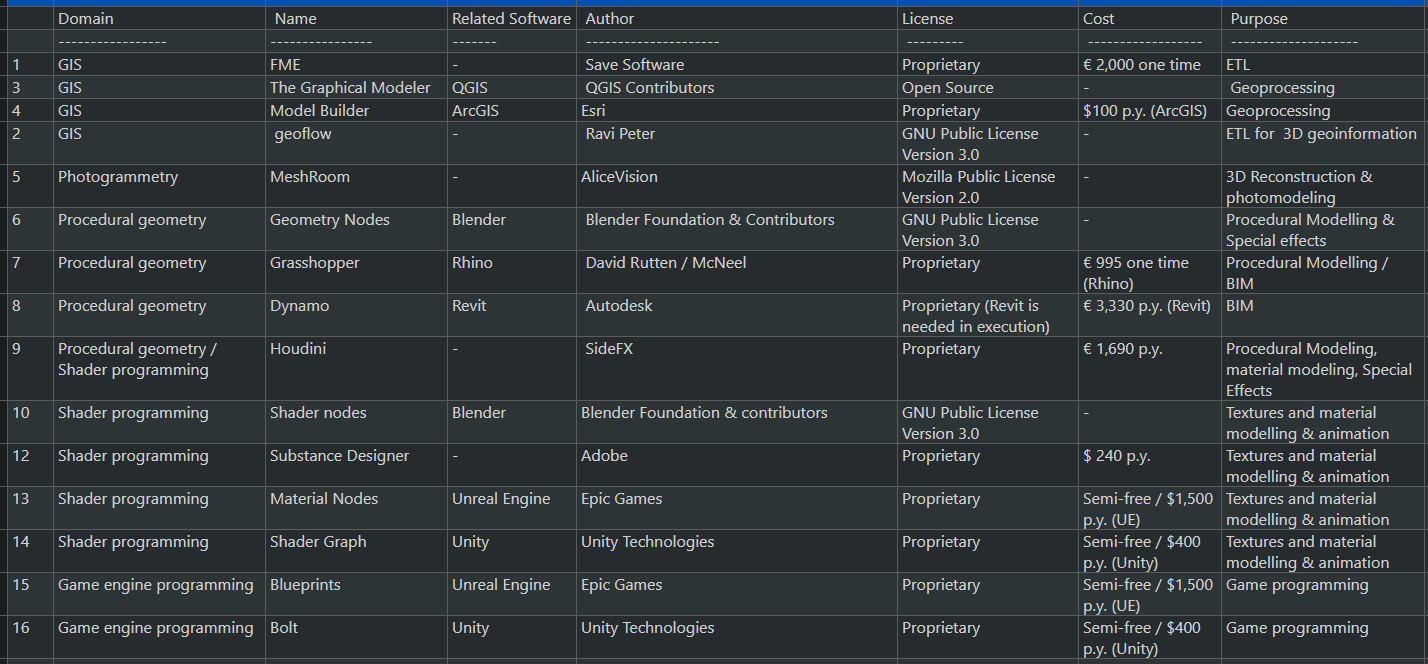
\includegraphics[width=400px]{geovpl.png}
  \caption{An overview of VPLs in the field of GIS and adjacent domains}
  \label{fig:geovpl:table}
\end{figure}

\subsection*{ VPLs in GIS }

Within the field of geo informatics, \ac{VPL}s are not a new phenomenon. VPLs have been used for decades to specify geodata transformations and performing spatial analyses.  

The most well-known visual programming language within the field of \ac{GIS} is the commercial \ac{ETL} tool FME \citep{safe-software_fme_2022}, (see \reffig{fig:gisvpl:1}). 
This tool is widely used by \ac{GIS} professionals for extracting data from various sources, transforming data into a desired format, and then loading this data into a database, or just saving it locally.  
FME is most often used within GIS to harmonize heterogenous databases, and as such specializes in tabular datasets. 

The two major GIS applications ArcGIS and QGIS also have specific \ac{VPL}s attached to their applications. 
The main use-case for these \ac{VPL}s is to automate repetitive workflows within ArcGIS or QGIS. 

Lastly, Geoflow is a much newer \ac{VPL} meant for generic 3D geodata processing \citep{peters_geoflow_2019}.
While this application is still in an early phase, it already offers a powerful 
range of functions.
It offers CGAL processes like alpha shape, triangulation and line simplification, as well as direct visualization of in-between products.
Geoflow was used to model the 3D envelope of a building based on a pointcloud, which was subsequently scaled up in the creation of the 3D BAG dataset \citep{peters_geoflow_2019}.

% In comparison with the three aforementioned \ac{GIS} vpls, geoflow is much richer 

\begin{figure}
\centering
\begin{subfigure}[b]{0.45\linewidth}
  \graphicspath{{../../assets/images/background/geo-vpl/}}
  \centering
  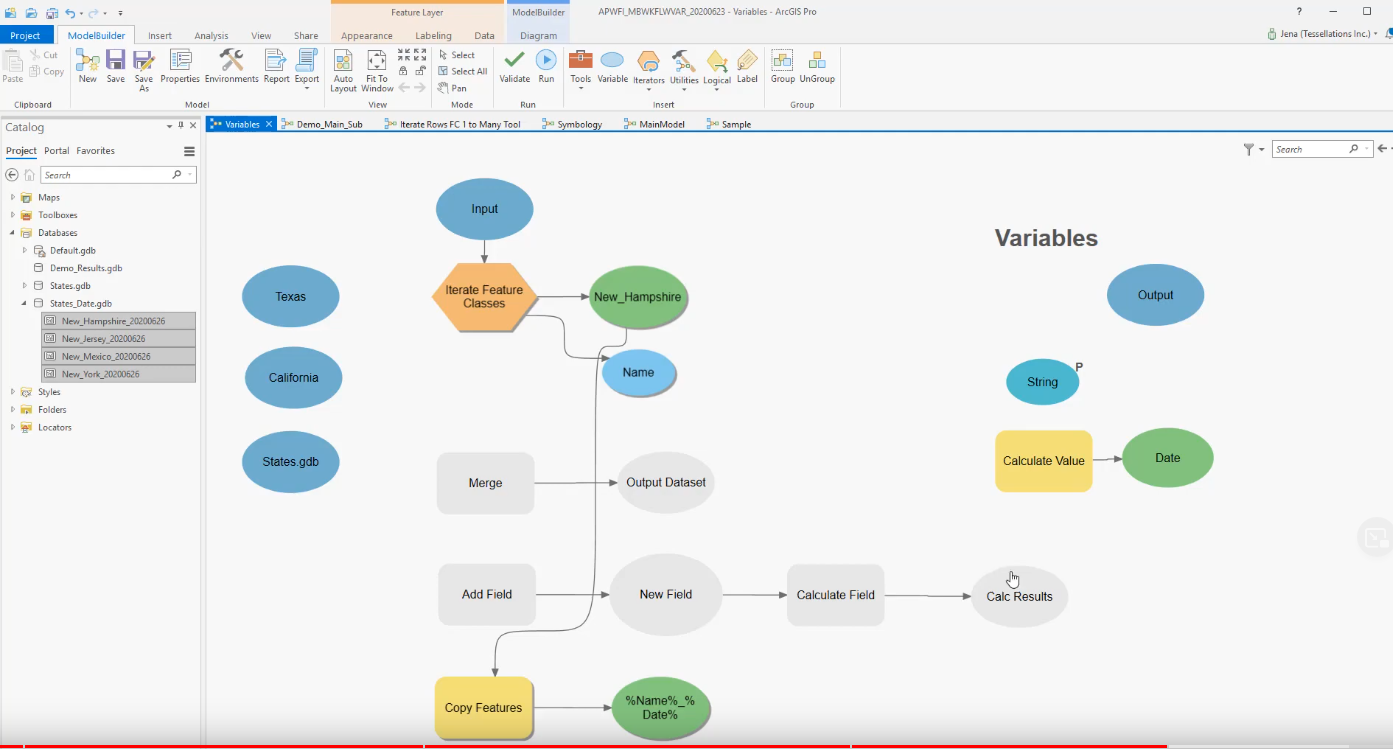
\includegraphics[width=\linewidth]{arcgis.png}
  \caption{}\label{fig:gisvpl:1}
\end{subfigure}%
\qquad 
\begin{subfigure}[b]{0.45\linewidth}
  \graphicspath{{../../assets/images/background/geo-vpl/}}
  \centering
  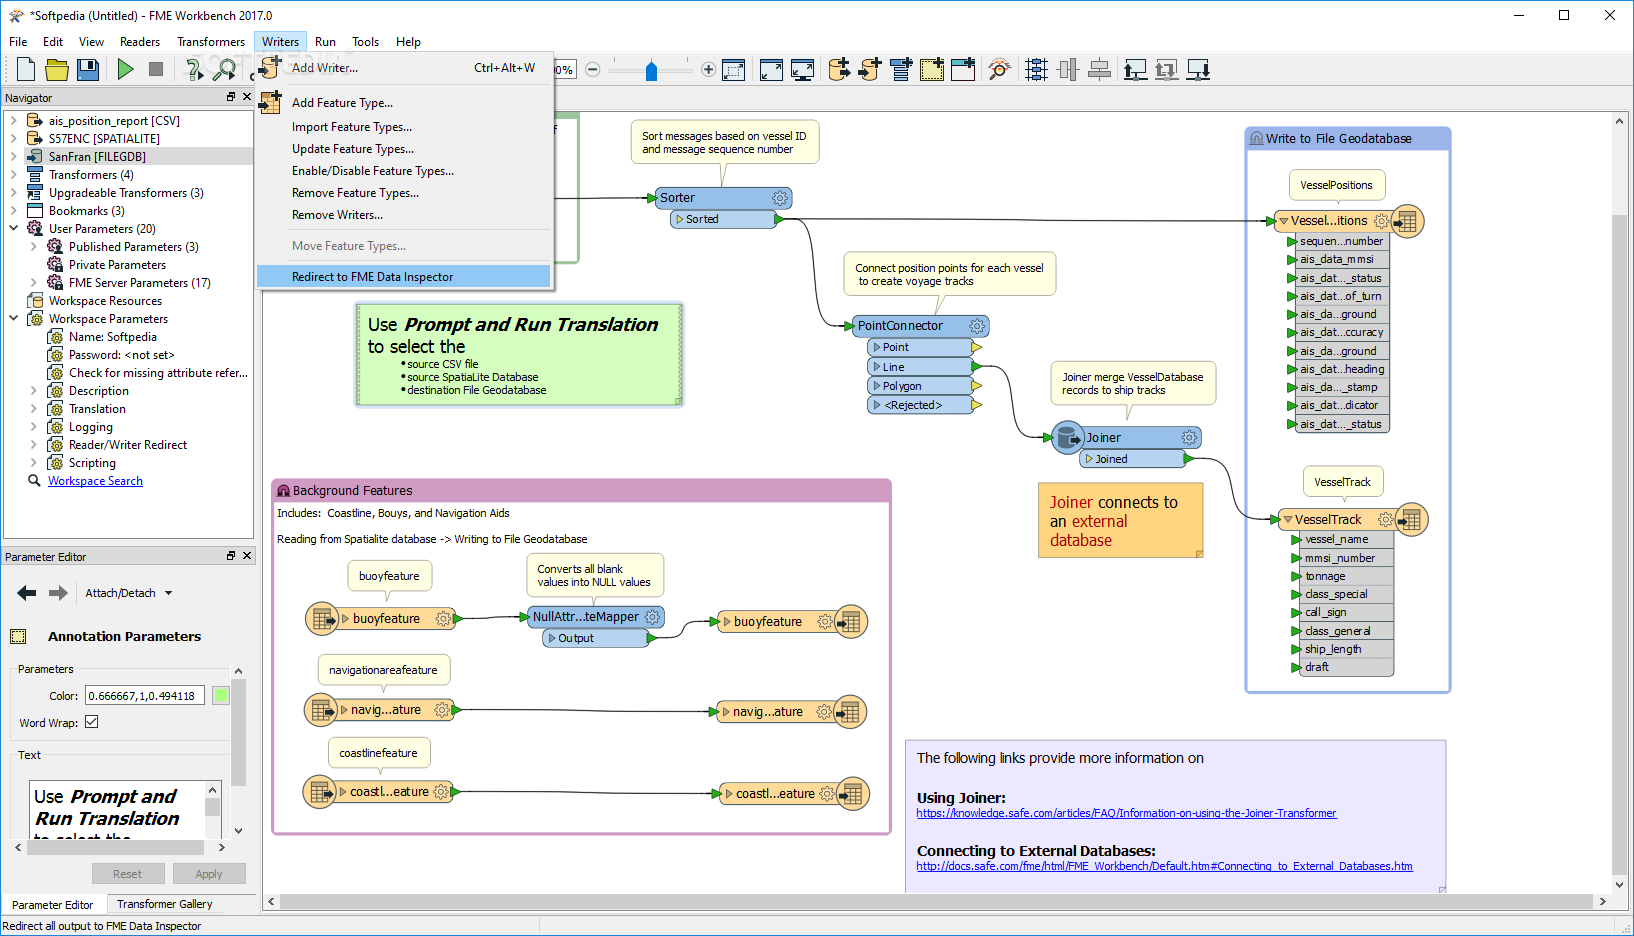
\includegraphics[width=\linewidth]{fme.png}
  \caption{}\label{fig:gisvpl:2}
\end{subfigure}%
\\
\begin{subfigure}[c]{0.45\linewidth}
  \centering
  \graphicspath{{../../assets/images/background/geo-vpl/}}
  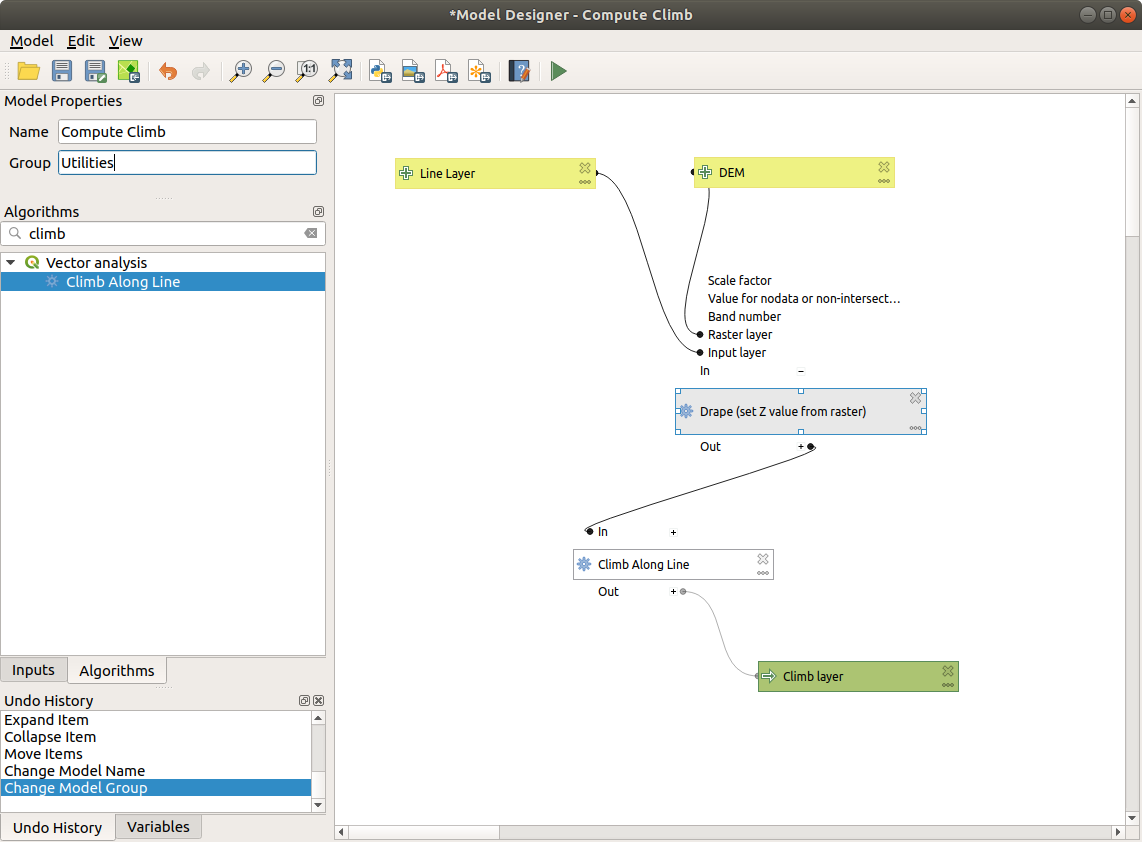
\includegraphics[width=\linewidth]{qgis.png}
  \caption{}\label{fig:gisvpl:3}
\end{subfigure}%
\qquad 
\begin{subfigure}[d]{0.45\linewidth}
  \centering
  \graphicspath{{../../assets/images/background/geo-vpl/}}
  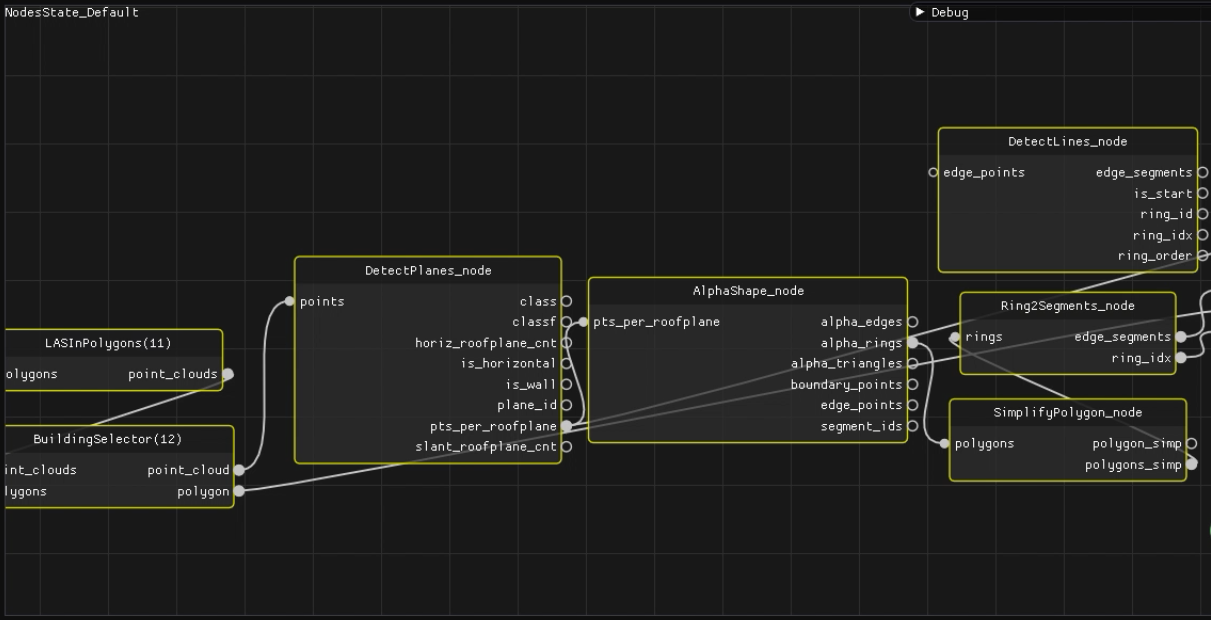
\includegraphics[width=\linewidth]{geoflow.png}
  \caption{}\label{fig:gisvpl:4}
\end{subfigure}%
\caption[GIS VPLs]{Four VPLs used in the field of GIS: 
ArcGIS's Model Builder \citep{esri_modelbuilder_2022} (a), 
Save Software's FME \citep{safe-software_fme_2022} (b), 
QGIS's Graphical Modeler \cite{qgis_community_qgis_2022} (c), 
and Geoflow \citep{peters_geoflow_2019} (d).}
\label{fig:gisvpl}
\end{figure}

\subsection*{ VPLs in neighboring domains }

\reffig{fig:geovpl:table} shows a great number of non-GIS \ac{VPL}s.
while these do not explicitly cover GIS, their close ties to computer graphics are still highly relevant to GIS and the activity of geocomputation.  

The choices of which vpl to include in \reffig{fig:geovpl:table} are based upon popularity.  
The particular ones chosen see a lot of use, evident by the sheer number of courses and tutorials which cover these vpls, and the popularity of the software packages these applications are attached to. 
In fact, many of the mentioned vpls are popular enough that it is safe to say that \ac{VPL}s are common in the wider field of computer graphics. 
This study limits itself to four sub-domains relevant to geocomputation:
\begin{itemize}[-]
  \item VPLs to calculate materials, shaders and textures
  \item VPLs to calculate geometry
  \item VPLs for photogrammetry 
  \item VPLs to calculate behavior and logic
\end{itemize}

\subsubsection*{Commonalities}
One interesting fact is that we see a great number of parallels among all these \ac{VPL}s.
\begin{itemize}[-]
  \item All are diagram-based vpls.
  \item All offer inspection of in-between products. Some even visualize data being parsed between nodes.
  \item All emphasize a process of "parametrization": parameters of various functions can be configured using sliders, curves, and other \ac{GUI} elements. This allows quick experimentation of different settings.
\end{itemize}
Moreover, the persistence of visual programming within these computer graphics fields, suggests that visual programming languages are advantageous for calculations dealing with 2D and 3D data.

The study speculates that this might be the case, because all these vpls, with exception to the behavior vpls, are essentially dealing with "functional data pipelines".
No distributed systems or event driven architectures, just one calculation from start to finish, to produce a desired product.  
However, the sheer amount of possible steps within these pipelines, together with the challenges of fine-tuning many relevant parameters, and the importance of inspecting in-between products visually, do not allow these pipelines to be configured by conventional UI's. 
However, a \ac{VPL} does deliver these features.
% vpls allow rapid debugging, rapid experimentation, and the straight-forward nature of 2D/3D pipelines mitigate the challenge vpls have with representing imperative flow statements (\m{if, else, for, while, break}). 

\subsubsection*{Material VPLs}
By far the most commonplace type of vpl present in computer graphics are material Vpls. 
In this context, the concept "material" often refers to a combination of 2D textures and shaders. 
These include PBR settings, normal maps, bump maps, and / or custom shader programs. 
The repetitive and time-consuming nature of manually creating textures, and the fact that some of these material properties can be inferred from each other, lead many CG applications to develop \ac{VPL}s for this particular purpose. 
3D artists use these \ac{VPL}s to create procedural materials.

\begin{figure}
  \centering
  \graphicspath{{../../assets/images/3/}}
  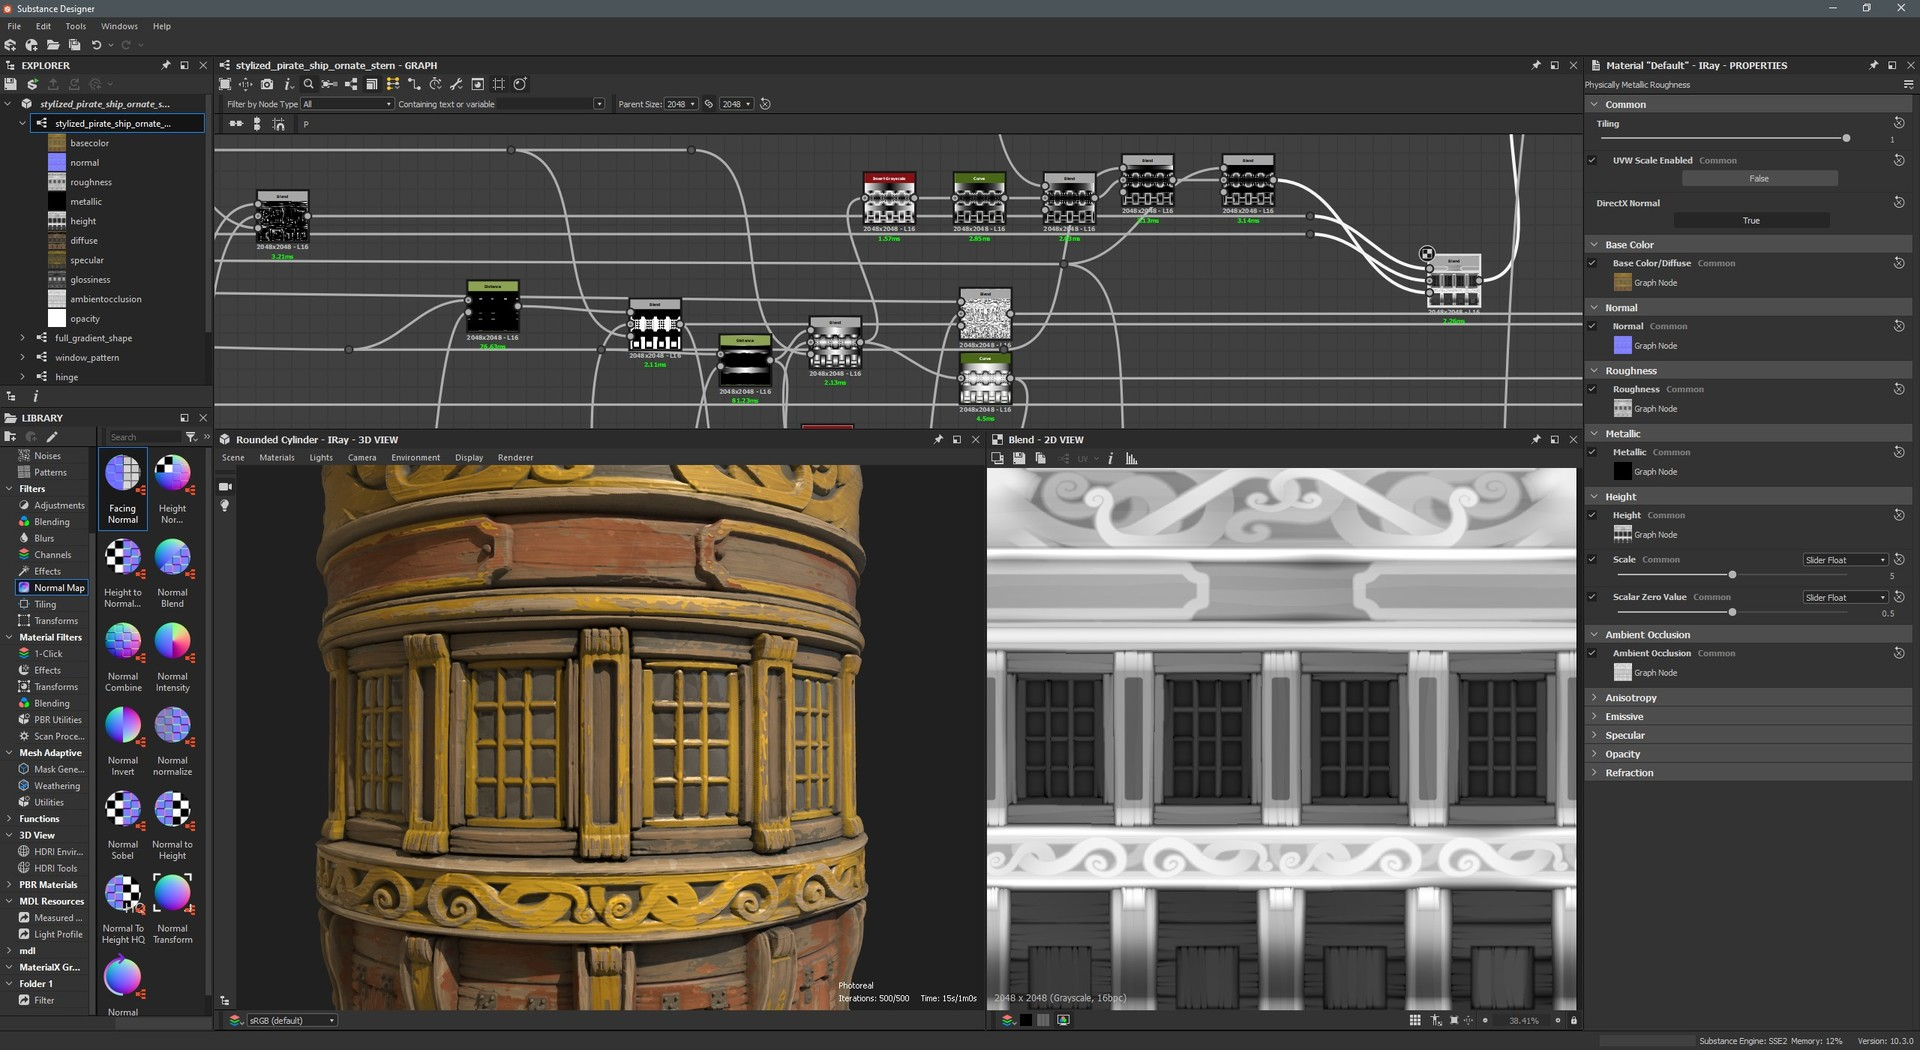
\includegraphics[width=\linewidth]{substance-designer.jpg}
  % actual source: https://store.steampowered.com/app/1454910/Substance_3D_Designer_2021/
  \caption[Geometry VPL]{Substance designer, a VPL for textures \citep{rutten_grasshopper_2012}}
  \label{fig:texture-vpl}
\end{figure}

\subsubsection*{Geometry, and photogrammetric VPLs}

Procedural Geometry \ac{VPL}s are not far behind the material \ac{VPL}s in terms of popularity.
Applications like Blender's geometry nodes \citep{blender_foundation_geometry_2022}, Rhino's Grasshopper \citep{rutten_grasshopper_2012}, or Houdini \citep{sidefx_houdini_2022}, are all widely used to automate the creation of geometry. 
Where Houdini and Blender's vpls are primarily used in games and special effects, Grasshopper sees usage in the Architecture, Engineering and construction industry. 
In this field, procedural geometry is often referred to as "parametric design".

Alicevision's Meshroom application must also be mentioned \citep{alicevision_meshroom_2022}.
While this can be regarded as procedural modelling, the complexity and computation involved in photogrammetry make a vpl offering it a class in of itself. 
The vpl inside of Meshroom can be used to fine tune all stages of the 3D reconstruction process.

\begin{figure}
  \centering
  \graphicspath{{../../assets/images/3/}}
  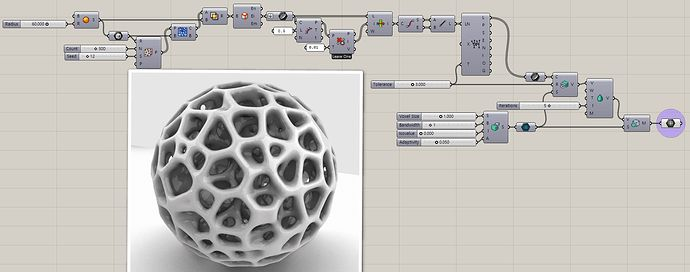
\includegraphics[width=\linewidth]{grasshopper.jpg}
  % actual source: https://global.discourse-cdn.com/mcneel/uploads/default/original/3X/a/5/a5b9354d24af2f4e25038357ac64476b02e1d966.png
  \caption[Geometry VPL]{Grasshopper, a VPL for geometry \citep{rutten_grasshopper_2012}}
  \label{fig:geo-vpl}
\end{figure}

\subsubsection*{Behavioral VPLs}
The behavioral and logical vpls found in applications such as Unreal's Blueprint \citep{epic_games_blueprints_2022} and Unity's Bolt \citep{unity_technologies_bolt_2021} are less relevant to the activity of geocomputation.
However, one interesting property worth mentioning, is that these languages have actually designed a way for end-users to define imperative flow statements, since these could not be overlooked for behavior and logic.
\refsec{sec:background-vpl} named conditions and loops as one of the challenges of diagram-based vpls. 
These languages both attempted to solve this problem by introducing a special "flow state" variable. 
It represents no value, but simply the activity of 'activating' or 'doing' the node selected. 
\reffig{fig:logic-vpl} showcases these flow-state variables in both languages using conditionals.
flow-state variables have their own set of rules, completely separate from connections carrying data. 
For example, they can be used cyclically, offering users looping functionality and are allowed to have multiple sources.  
Despite these functionalities, one might wonder if these aspects are worth these extra complications.
Especially since these flow-state variables are effectively \m{GOTO} statements, which are widely known as an anti-pattern in large-scale software projects. 

\begin{figure}
\centering
\begin{subfigure}[b]{0.45\linewidth}
  \graphicspath{{../../assets/images/background/geo-vpl/}}
  \centering
  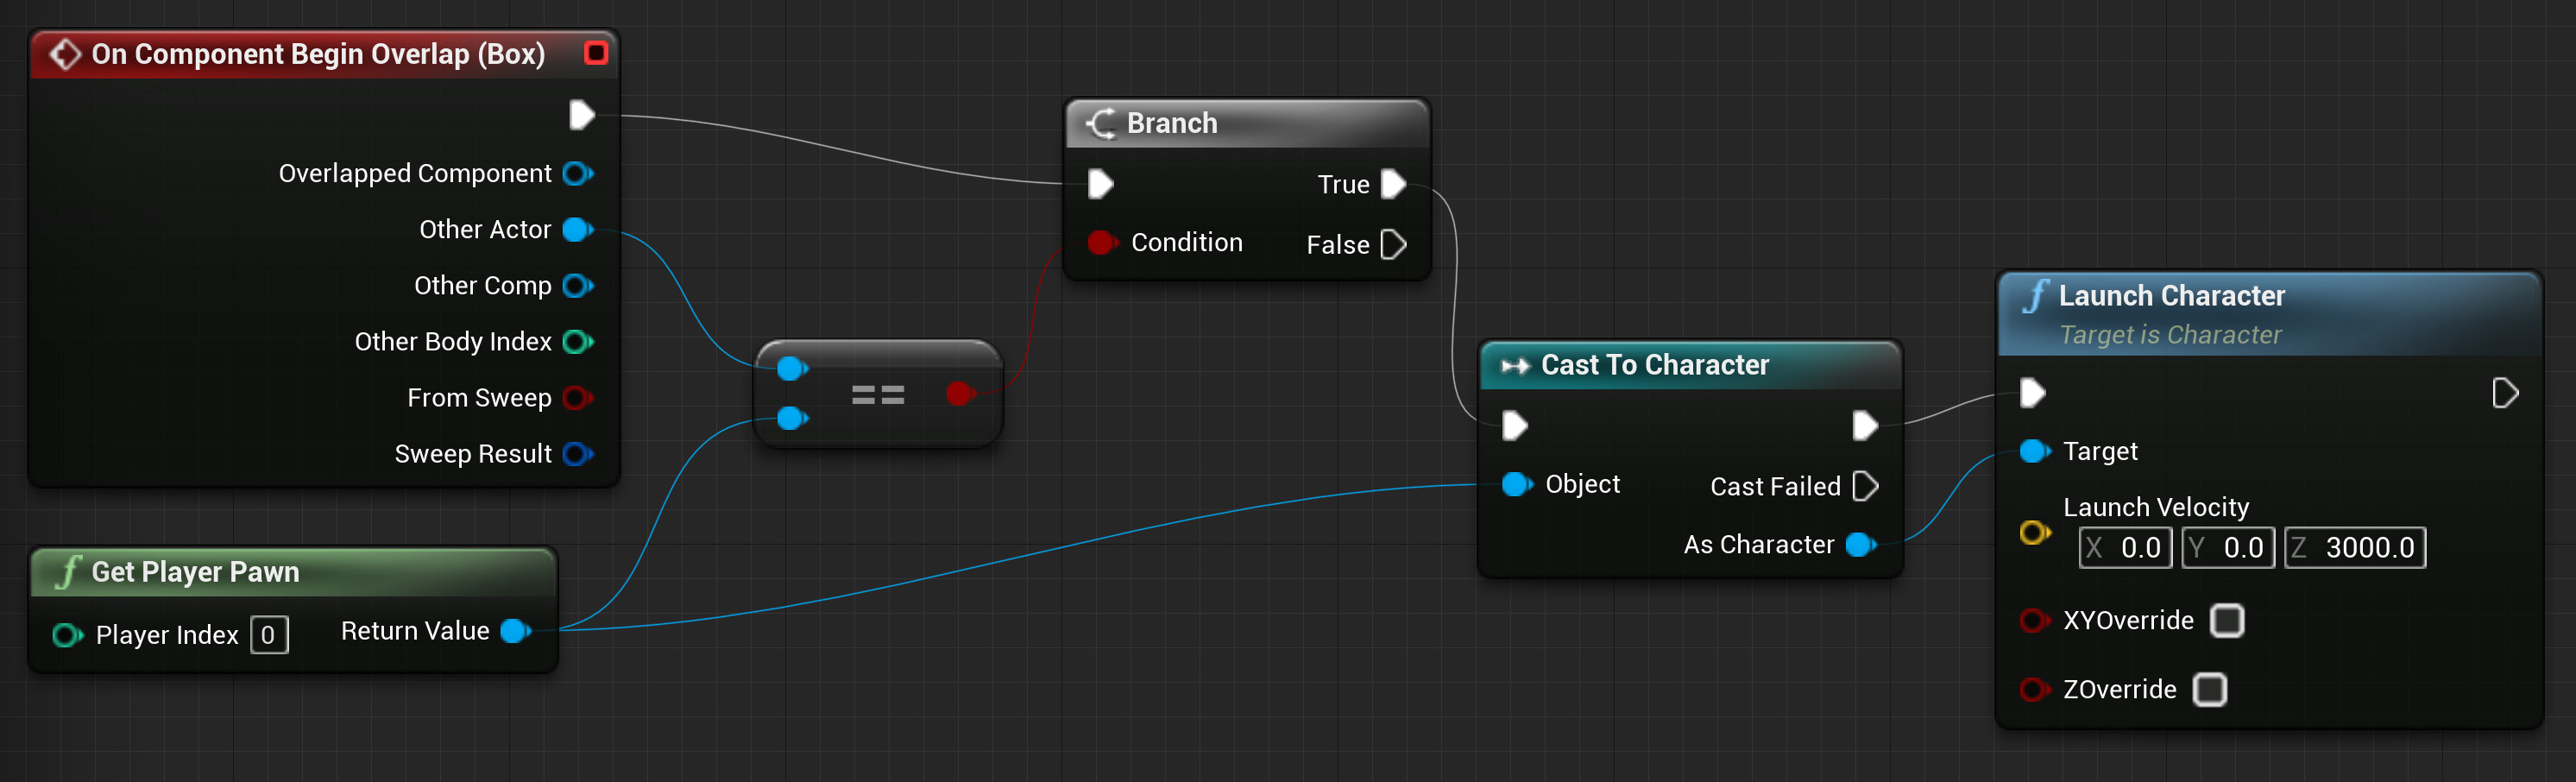
\includegraphics[width=\linewidth]{unreal-blueprints.jpg}
  \caption{}\label{fig:logic-vpl:1}
\end{subfigure}%
\qquad %-- that adds some space between th 2 figures
\begin{subfigure}[b]{0.45\linewidth}
  \graphicspath{{../../assets/images/background/geo-vpl/}}
  \centering
  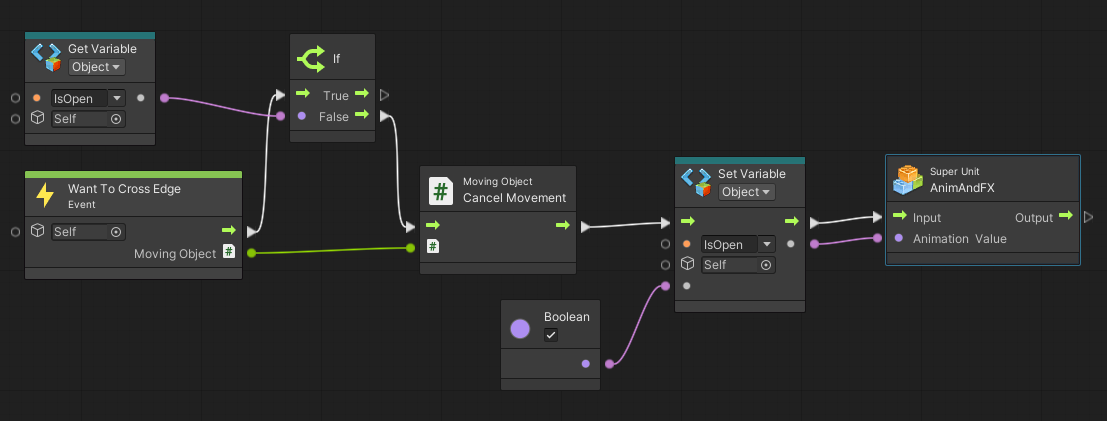
\includegraphics[width=\linewidth]{unity-bolt-2.png}
  \caption{}\label{fig:logic-vpl:2}
\end{subfigure}%
\caption[Behavioral VPLs]{Two VPLs for logic, showing "flow-state" variables. Left: Unreal's Blueprints, Right: Unity's Bolt. \citep{epic_games_blueprints_2022, unity_technologies_bolt_2021}}
\label{fig:logic-vpl}
\end{figure}

\section{Browser-based visual programming}
\label{sec:related-webvpl}

This section is dedicated to visual programming applications running in a browser.
It must be emphasized that of all the various vpls named in \refsec{sec:related-geovpl}, none are browser-based. 
This is likely the case because most of those vpls are computationally intensive, C++-based applications.

Nevertheless, if one looks in other domains, we quickly see many \ac{VPL}s which are web-based. 
Out of all 30 VPL studies covered by the meta analysis of \cite{kuhail_characterizing_2021}, 17 were web based, 7 were mobile based, and only 6 were desktop applications. 
Kuhail et al. continue by noting that most of these 6 desktop applications were build during or before 2013. 
The reason Kuhail et al. give for this stark difference is in line with research covered in \refsec{sec:background-web}: 
\emph{"This can be explained by the fact that desktop-based tools are cumbersome to contemporary users. They must be downloaded and installed, are operating-system dependent, and need frequent updates."}.

\begin{figure}
\centering
\begin{subfigure}[b]{0.45\linewidth}
  \graphicspath{{../../assets/images/background/web-vpl/}}
  \centering
  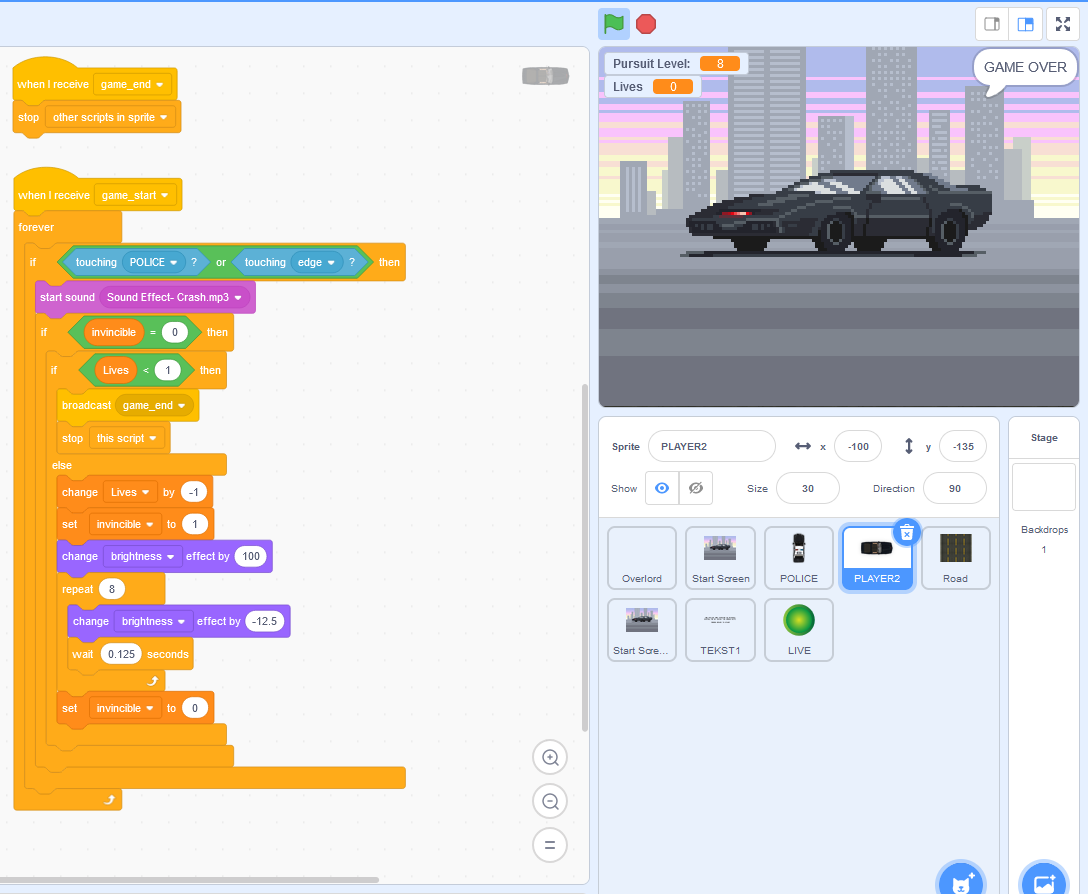
\includegraphics[width=\linewidth]{scratch-2.png}
  \caption{}\label{fig:webvpl:1}
\end{subfigure}%
\qquad 
\begin{subfigure}[b]{0.45\linewidth}
  \graphicspath{{../../assets/images/background/web-vpl/}}
  \centering
  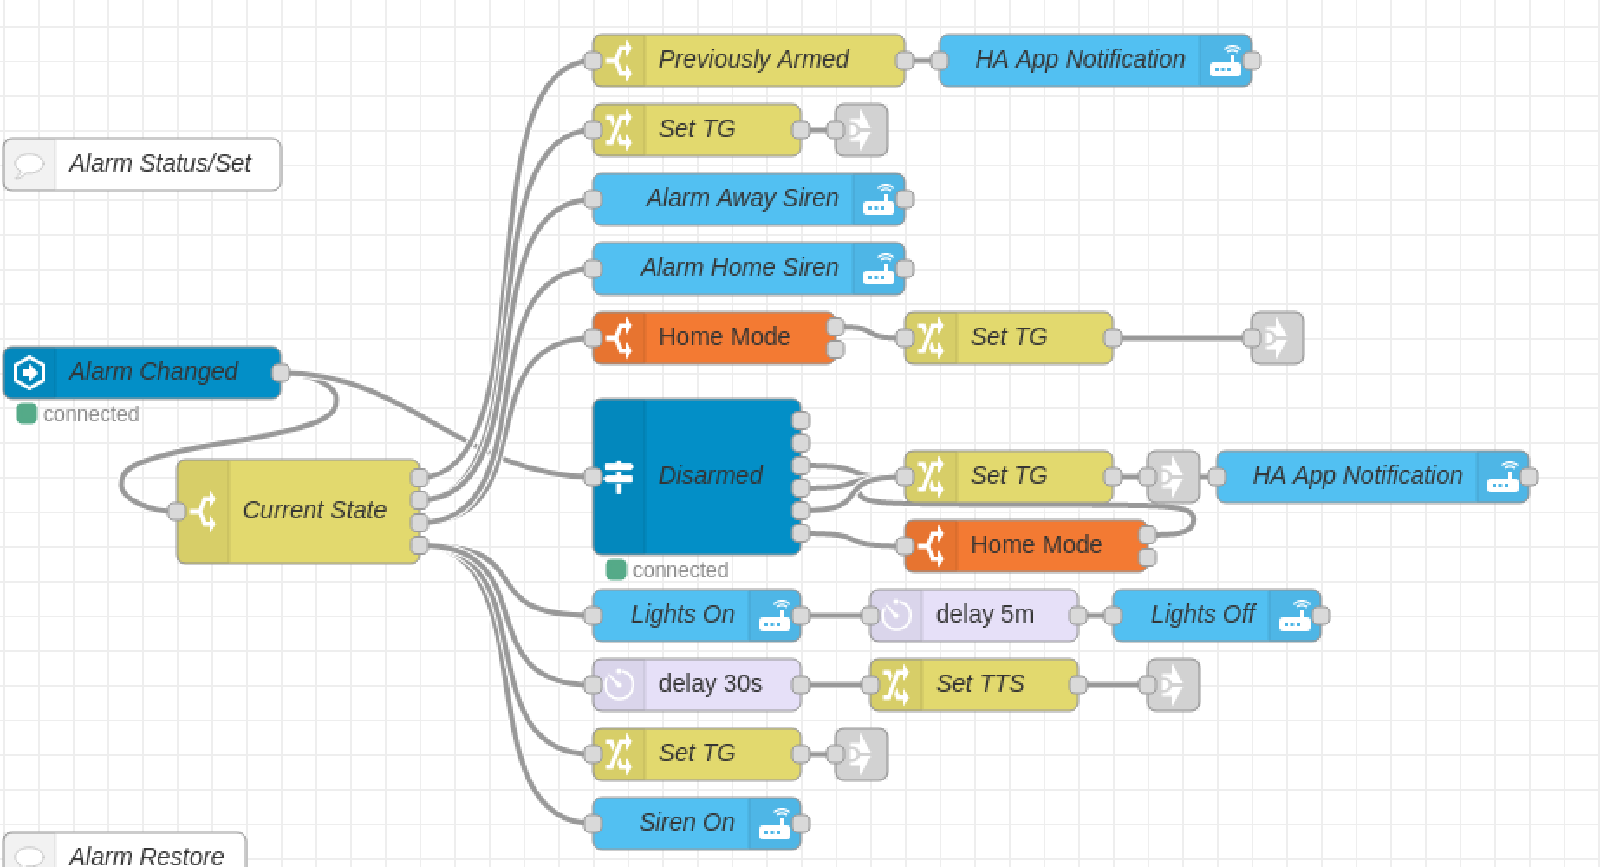
\includegraphics[width=\linewidth]{nodered-2.png}
  \caption{}\label{fig:webvpl:2}
\end{subfigure}%
\caption[web VPLs]{Two VPLs used on the web: Scratch (a) \citep{resnick_scratch_2009}, and nodeRED (b) \citep{openjs_foundation_node-red_2022}. }
\label{fig:webvpl}
\end{figure}

% (SOURCE: https://dl.acm.org/doi/fullHtml/10.1145/1592761.1592779?casa_token=cJ1iX1YYimkAAAAA:YVyp3KFiKwD2GMuBUUIgvibbNsEgndqNQzehRnCosCpyEx51C_uNpi2D4-lsE-x88hQFSWcbTfrP_w)
% (https://www.ucode.com/coding-classes-for-kids/is-scratch-the-same-as-blockly)
% (https://developers.google.com/blockly/)
% (https://developers.googleblog.com/2019/01/scratch-30s-new-programming-blocks.html)
This study wishes to present two web based visual programming languages, which each use the web in a meaningful way.  
The first web-vpl is "Scratch" \citep{resnick_scratch_2009} (See \reffig{fig:webvpl:1}). 
Scratch is well-known as an educational, block-based vpl, targeted at children and young adults to teach the basics of computational thinking.   
As noted by the authors of CS50, scratch is, despite this target audience, surprisingly close to any normal programming language, with for and while loops, if statements, and even event handling and asynchronous programming. 
Scratch used to be a desktop application. 
The web environment this vpl now occupies allows its users some life-cycle support. 
Users can immediately publish their work, search for and run the work of others, and even "Remix / clone / fork" the source code of these other projects. 
This encourages users to learn from each other.

% [blockly-> can be compiled to python and javascript]
% Microsoft makecode arcade

The second exemplary web vpl this study wishes to bring to the readers attention is the "nodeRED" application \citep{openjs_foundation_node-red_2022} (see \reffig{fig:webvpl:2}). 
This is a feature-rich diagram-based application, created to serve the domain of IoT.
This vpl uses the browser-based platform not only for the aforementioned \refsec{sec:background-web} reasons, but also for the exact same reasons a router, NAS or IoT device often opts for a browser-based interface: 
Servers, either small or big, explaining how they desire to be interfaced, is more or less the cornerstone all web clients are based upon.  
If the server serves its corresponding client, users do not need to find some compatible interface themselves.
For this reason the "nodeRED" application is a web application, even though it is mostly run on local networks.   

\section{Browser-based geocomputation using a VPL} 

% - Mobius Modeller : https://mobius.design-automation.net/pages/mobius_modeller.html
To the best of the author's knowledge, only one publicly available visual programming language exist which is both able to be configured and executed in a browser, and is able to be used for geodata computation.
This application is called the Möbius Modeller \citep{janssen_mobius_2021}, and is the closest equivalent to the geo-web-vpl proposed by this study.
Though it only uses javascript, the tool is able to be successfully used for a number of applications, including CAD, BIM, urban planning, and GIS. 
It uses a combination of a 'bare-bones' diagram-based vpl, together with a rich block-based vpl (See \reffig{fig:mobiusmodeller}).
In fact, the block-based vpl is so rich that is almost ceases to be a vpl altogether, and starts to be python-like language with heavy IDE support.  

The VPL proposed by this study still differs from the mobius modeller in the following ways: 
\begin{itemize}[-]
  \item This study explores the usage of a pure dataflow VPL, as opposed to the multiple types of VPLs used by the Möbius Modeller. This is done to allow for the dataflow programming advantages described in \refsec{sec:background:dataflow}.
  \item This study explores the usage of WebAssembly to hypothetically improve performance and to use existing geocomputation libraries.
  \item This study addresses some of the life-cycle issues of \ac{VPL}s stated in \refsec{sec:background:vpl:disadvantages}. 
\end{itemize}

\begin{figure}
  \centering
  \begin{subfigure}[b]{0.45\linewidth}
    \graphicspath{{../../assets/images/background/geo-web-vpl/}}
    \centering
    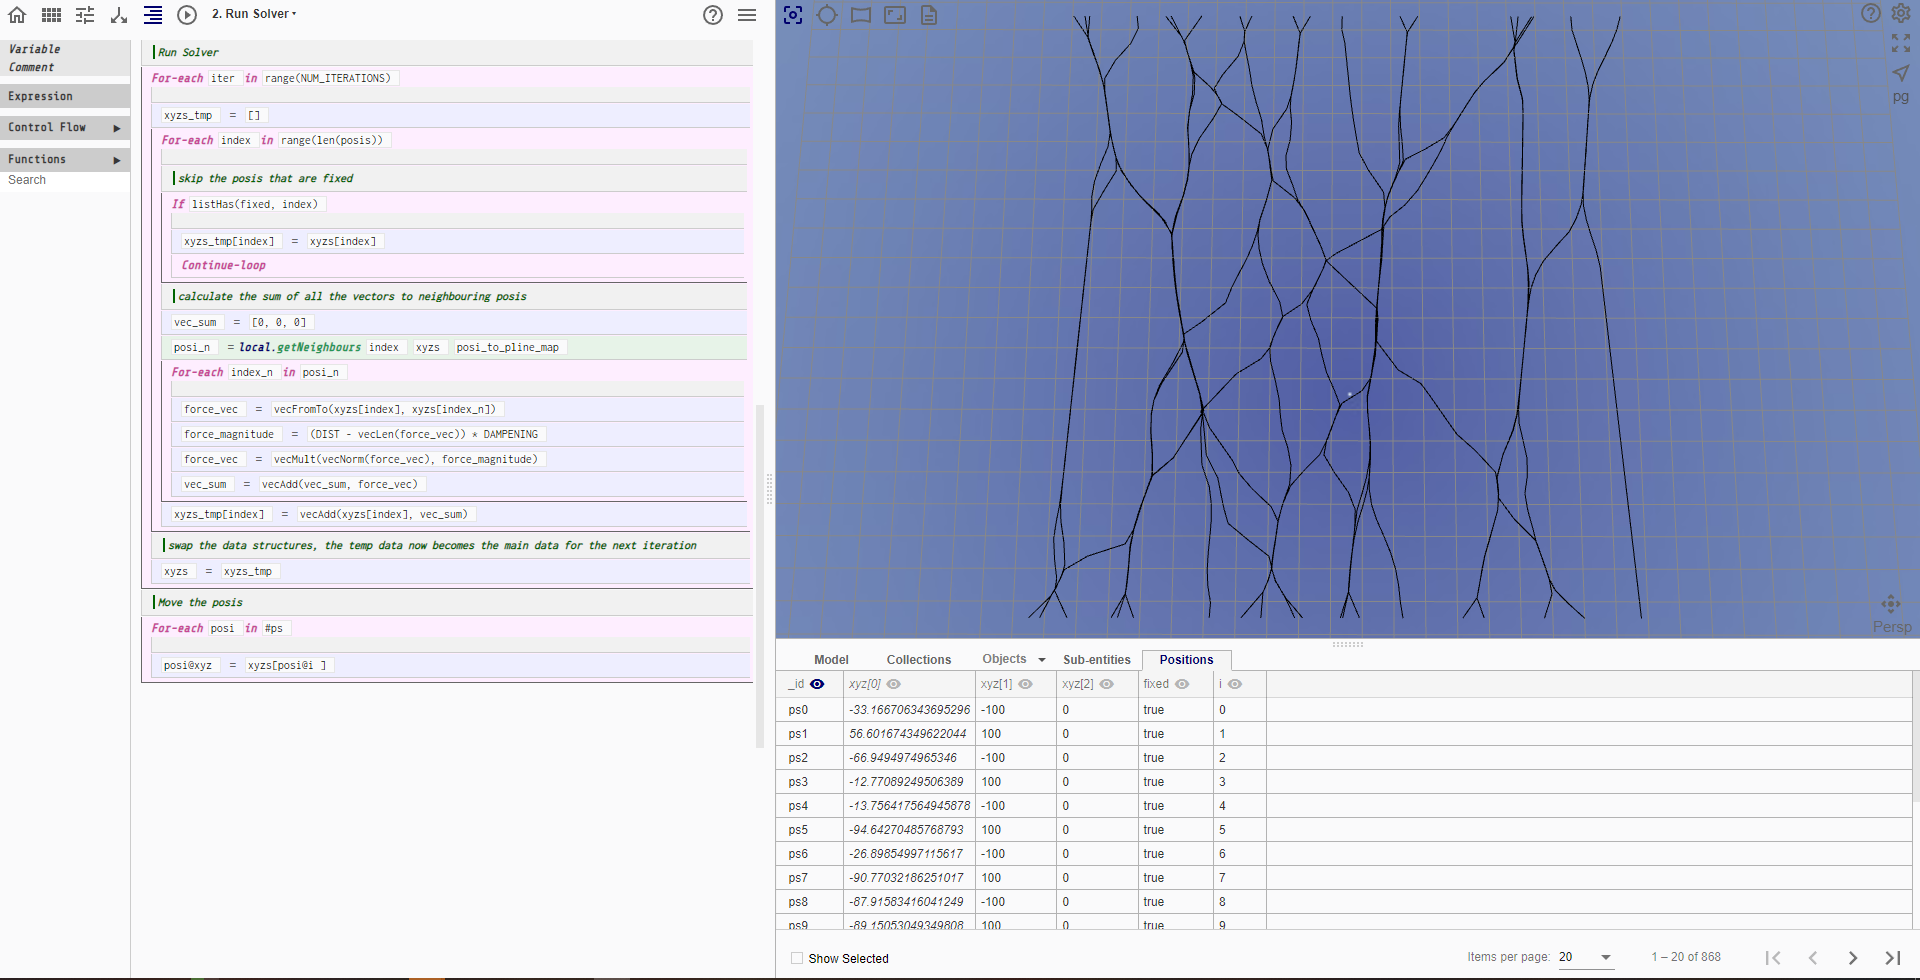
\includegraphics[width=\linewidth]{mobius-3.png}
    \caption{}
  \end{subfigure}%
  \qquad %-- that adds some space between th 2 figures
  \begin{subfigure}[b]{0.45\linewidth}
    \graphicspath{{../../assets/images/background/geo-web-vpl/}}
    \centering
    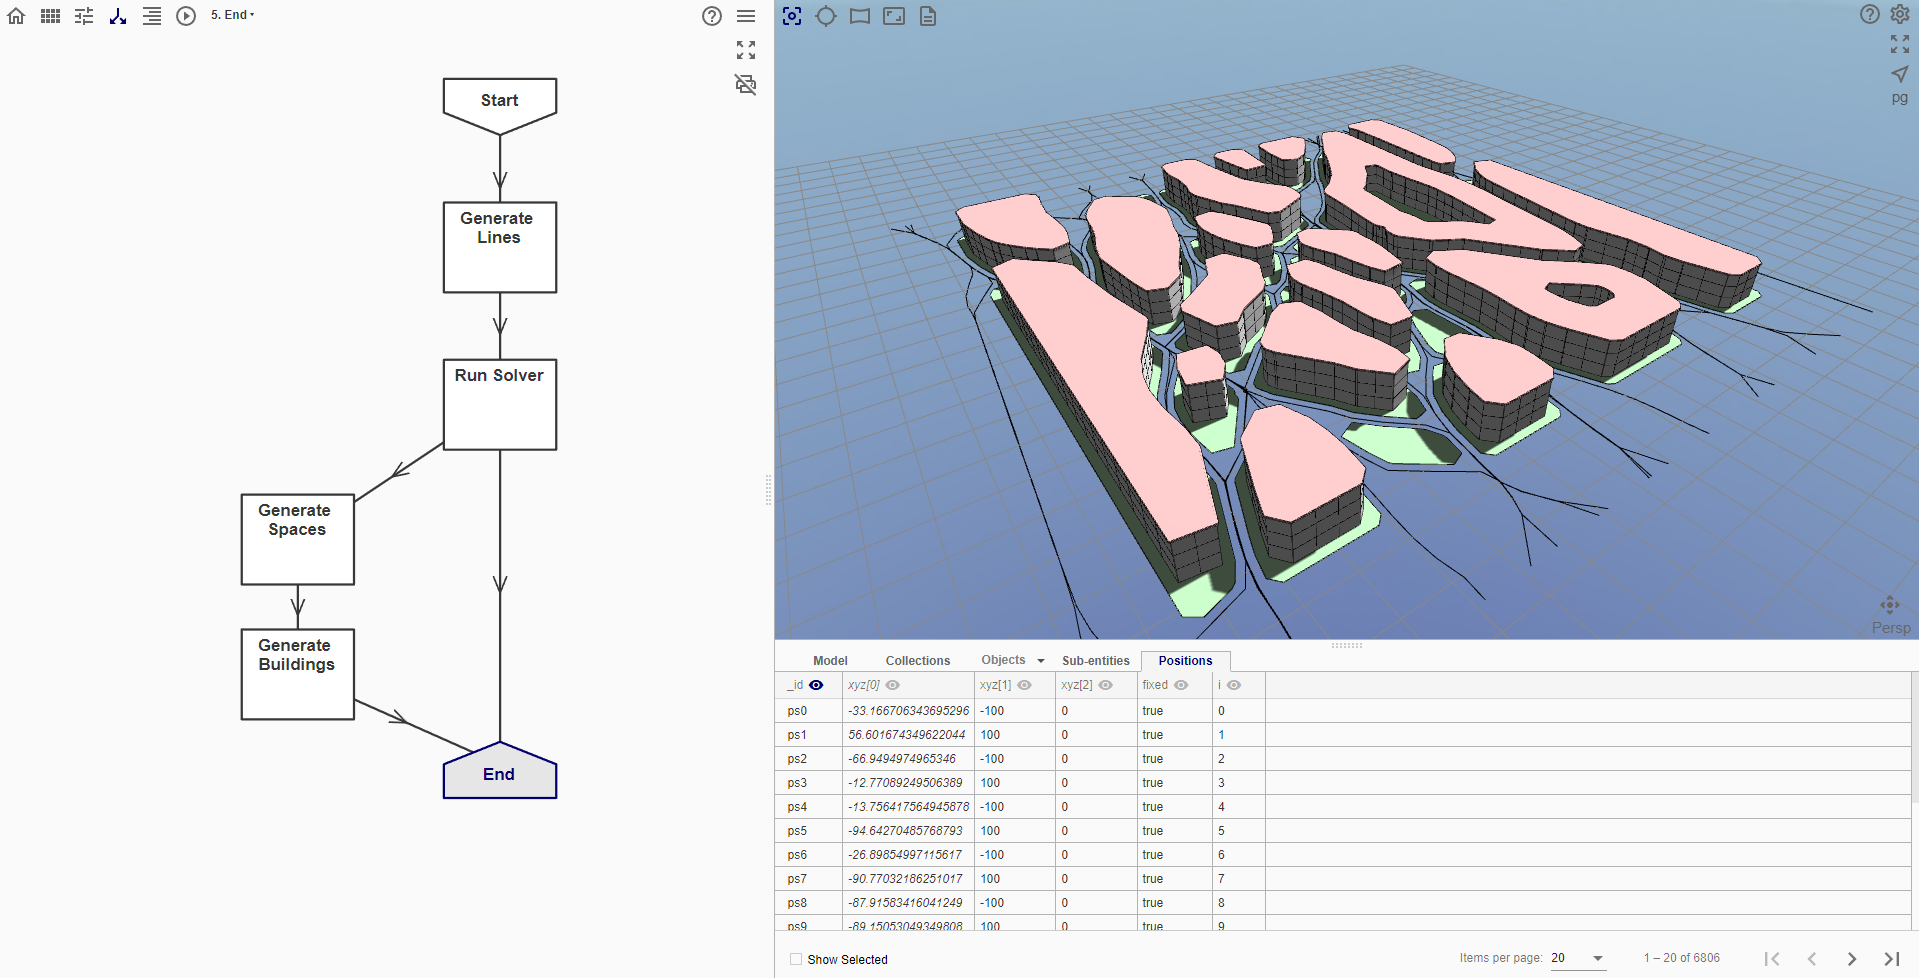
\includegraphics[width=\linewidth]{mobius-4.png}
    \caption{}
  \end{subfigure}%
  \caption[Mobius Modeller]{Images of the Mobius modeller application \citep{janssen_mobius_2021}}%
  \label{fig:mobiusmodeller}
  \end{figure}

%% SOME THOUGHTS ON RELATED WORKS: 

% GEO: the thing we want to do
% VPL: best choice for end user development, 
% WEB: solves the huge life-cycle problem of publication


% SOME THOUGHTS ABOUT THE IMPORTANCE OF EXPERIMENTATION AND PLAY
% -> testing & reproducability.
% RANSAC -> many 'magic' parameter. 
% Game Of Life -> impossibility of 'proving' behaviour systems. 
% Many parameters simply need to be discovered by 'play' / simulation
% Jonathan blow -> using interactive applications, an intrinsic understanding can be gained without explicit communication.

% gdevelop 
% Define the scope, extend, and how of the study
\chapter{Methodology}
\label{chap:methodology}

This chapter explains the methodology used in this study. 
The overall structure of what elements this methodology precisely consists of is presented, and how these elements came to be. 
The chapter continues with four sections, each explaining one of these components.
But first, I wish to clarify the nature in which this study is conducted. 

\subsection*{Nature}
The methodology of this study can be characterized as practical as opposed to theoretical, wholistic instead of specific, and iterative compared to linear. The prior works on browser-based geocomputation and geo-vpls indicate that a strong theoretical framework for a \ac{geo-web-vpl} is in place (Source). 
But, and this is especially evident in the prior studies regarding \ac{bbg} (Source), the practical implementation of these theories were only partially successful, and limited in scope. 
This necessitates a practical, wholistic approach in response. 
And, due to the investigative nature of this study, the methodology requires to iterate upon itself, instead of following a singular, linear path. 

% ...
% % Theorie: is er maar je geloofde het niet
% % praktische implementatie om de Throerie weerleggen
% The prior works on browser-based geoprocessing indicate that a theoretical framework for browser-based geoprocessing vpl is in place. 
% But, and this is especially evident in the studies regarding client-side geoprocessing, the practical implementation of these theories

% Choices: 
% - practical > theoretical : Literature study indicates enough theoretical soundness, but lots of practical questions remaining. We wish to  immediate pick up where these studies have left, and therefore we choose the direct, practical study of designing and implementing a prototype application. 
% - wholistic > specific    : Research in one sub-domain could have been more exhaustive in one of the specific sub-studies, instead of covering the full scope it does now. However, This would have been incomplete. What we do now is cover the full pipeline of using a geocomputation library: from creation to web export, to web import, to web utilization. by doing this, we can identify issues caused in one of these
% - iterative > linear      : Given this vast scope, many questions can come up from different angles. The study has to be dynamic to adapt to these demands. 

\subsection*{Structure}
  
\emph{The content of this methodology is based upon the main and supporting research questions. 
As such, it bears fruit to explain how these specific questions were chosen.}

% FIX THISSS 
The related studies in \refchap{chap:related} show that only one \ac{geo-web-vpl} as described by this study exists. This is in contrast to the many examples of geo-vpls in \refsec{sec:related-geovpl} and web-vpls \refsec{sec:related-webvpl}. 
Based on this, it can be assumed that creating a visual programming environment in a web-browser must be possible. 
Using a \ac*{vpl} for geocomputation must also be possible. 
However, the greatly reduced number of geo-web-vpls indicates some sort of hinder, preventing this type of application to be realized. Either geo-VPLs were not able to be properly used in a browser, or web-based VPLs were unable to support geocomputation functionalities. 
% Assuming, of course, that researchers and developers of these environments would have wanted to work towards a \ac{geo-web-vpl}.

This study starts from the second assumption: 
Apparently, web-based VPLs are unable to support existing geocomputation functionalities. 
This could be because of several reasons, of which this study identifies four major ones.

geocomputation functionalities might not be able to be properly:
\begin{itemize}[-]
  \item \textbf{compiled} into a format functional on the web
  \item \textbf{loaded} within a web-based VPL
  \item \textbf{visualized} by the interface of a web-based VPL
  \item \textbf{used} within a web-based VPL
\end{itemize}
As it is unknown which one of these reasons ( or which combination of reasons ) is causing this barrier, the study must encompass all four of these possible hindrances, and access to what extend these aspects form a hinder towards the main goal of a \ac{geo-web-vpl}. 
Moreover, the real reason might not lie in one of these areas, but in the interplay between all of these factors. 

It is this study's objective to pose a solution to this barrier. This is stated by the main research question: \myMainRQ 

The study goes about doing so, by developing a prototype \ac{geo-web-vpl}. 
This prototype is used as a staging ground to discover the extend of possible hindrances. 
During its development, each one of these four possible hindrances has to be accounted for. 
Per hindrance, we document design considerations, and run experiments, all to test to what extend this prototype \ac{geo-web-vpl} fails or succeeds to provide for this aspect. 
After this is done, we can compile a final conclusion to the main research question. 

The methodology of this study is structured to facilitate this process. 
It is subdivided into four components, each representing a sub-research question, which is in turn based upon one of these possible hindrances. The questions are posed in such a way that answering them will require us to explore the extend of the hindrance, and find possible solutions.

The remained of this chapter covers the four components of this methodology, and how this relates to this prototype. 

\begin{note}
TODO: diagram: 4 research questions -> four possible barriers of geocomputation
\end{note}

\begin{note}
TODO: diagram: show the 'locations' of the four research questions ( client / server / native, etc.)
\end{note}

%%%%%%%%%%%%%%%%%%%%%%%%%%%%%%%%%%%%%%%%%%%%%%%%%%%%%%%%%%%%%%%%%%%%%%%%%%%%%%%%%%%%%%%%%%%%%%%%%%%%%%%%%%%%%%
%%%%%%%%%%%%%%%%%%%%%%%%%%%%%%%%%%%%%%%%%%%%%%%%%%%%%%%%%%%%%%%%%%%%%%%%%%%%%%%%%%%%%%%%%%%%%%%%%%%%%%%%%%%%%%
%%%%%%%%%%%%%%%%%%%%%%%%%%%%%%%%%%%%%%%%%%%%%%%%%%%%%%%%%%%%%%%%%%%%%%%%%%%%%%%%%%%%%%%%%%%%%%%%%%%%%%%%%%%%%%
%%%%%%%%%%%%%%%%%%%%%%%%%%%%%%%%%%%%%%%%%%%%%%%%%%%%%%%%%%%%%%%%%%%%%%%%%%%%%%%%%%%%%%%%%%%%%%%%%%%%%%%%%%%%%%
%%%%%%%%%%%%%%%%%%%%%%%%%%%%%%%%%%%%%%%%%%%%%%%%%%%%%%%%%%%%%%%%%%%%%%%%%%%%%%%%%%%%%%%%%%%%%%%%%%%%%%%%%%%%%%

\section{\mySubRQOneTitle} 
\label{sec:method-one}

The first component of the methodology involved the creation of the core of the prototype application, encompassed by the supporting research question : \mySubRQOne

% [WHY]
Before exploring how lifting \emph{existing} geo-computation to the web might take place, this study first wished to discover to what extend the web browser is able to facilitate the interface of a 3D vpl in general, both in terms of data structures and visualization. 
A 3D VPL is defined as a vpl meant for generic 3D geometry processing.

% [HOW]
The method to answer this question is defined as follows. 
The above question of \mySubRQOneTitle is further subdivided into 4 follow-up questions:
\begin{enumerate}[A]
  \item \emph{What are the requirements of a 3D VPL?}
  \item \emph{What can be defined as 'core browser features'?}
  \item \emph{Per requirement, to what extend can these core browser features be used to implement this requirement?}
  \item \emph{Per implemented requirement, to what extend does this web implementation differ from existing, popular 3D VPLs?}
\end{enumerate}

Question A and B will be answered subsequently. 
The question C is answered by \refsec{sec:app}, and the answer to the fourth question can be found in the Conclusion, as it doubles as the answer to the entire question of \mySubRQOneTitle.

\subsection*{A: 3D VPL requirements}

Based on the vpl research of \refsec{sec:background-vpl}, any visual programming language must at the very least contain the following aspects: 
\begin{enumerate}[-]
  \item a visual language
  \item an interface to configure this visual language 
  \item a representation of the 'variables' and 'functions' of the visual language
  \item a way to provide input data 
  \item a way to execute the language
  \item a way to display or save output data
\end{enumerate}

Based on popular, existing 3D vpl's (Blender, Unreal, Grasshopper) A visual programming language handling 3D data should have:
\begin{enumerate}[-]
  \item A method to preview 3D data used throughout the flowchart
  \item multiple ways to determine input data (text fields, sliders) 
  \item multiple ways to view output data (text displays, 3D viewers, etc.)
\end{enumerate}

A VPL also has many requirements which cannot be listed, but instead refer to the shaping of the entire application. 
For example, interactivity a defining factor of a vpl. GUI elements should be as interactive as possible.
However, aspects like this are hard to define or measure, and will not be included as part of this component of the methodology. 

% \begin{note}
%   Figure out what to do with this: 
 
%     Interactivity is the defining factor of the vpl. 
%     a list of standard VPL features & application features required as a base-line:  
%   - Users must be able to construct a script by visual means.
%   - Dataflow Modelling
%   - Dragging and dropping is a ui which

%   (geo-vpl features:)
%   - read data from user-submitted files
%   - write data to files, downloadable by the user  
%   - debug / inspect data in a 3D viewer
%   - draw geometry in a 3D viewer
% \end{note}

\subsection*{B: Core browser features}
This study defines "Core browser features" as the set of default features implemented by the three largest browser engines. 
\begin{note}
TODO: a pie chart of usage statistics
\end{note}
Based on these (FIGURE) market share statistics, the following three browsers engines appear to be the largest:
\begin{enumerate}[-]
  \item Chromium (Chrome, Edge) (Source)
  \item Gecko (Firefox) (Source)
  \item WebKit (Safari) (Source)
\end{enumerate}

The set of features common in all three browser engines are documented on (SOURCE: Mozilla). 
This includes the following set of features relevant for the 3D VPL:
\begin{enumerate}[-]
  \item WebGL (WebGL2, WebGPU)
  \item 2D Canvas API
  \item Web Workers
  \item Web Components
  \item WebAssembly
\end{enumerate}

\subsection*{C: Implementation Steps}

\begin{note}
TODO: An image showing the phases of development
\end{note}

To find the answer to question C, this study implemented the core of the prototype \ac{geo-web-vpl}.
Just like the entire study, the development trajectory for implementing will be done incrementally, ensuring results during all steps of the development. 
The first step of the phase consists of creating the basics of the \ac{gui} itself. 
A basic \ac{vpl} will be created which can only process boolean statements. 
The second step involves developing the main datamodel of the VPL, to represent the program in an object-oriented way. 
The third step adds types, geometry, and the visualization of this geometry in 3D, as well as textures / images in 2d. \
The fourth step adds geospatial data support, and adds Web Feature Services, Web Map Services, and coordinate reference systems.  

%%%%%%%%%%%%%%%%%%%%%%%%%%%%%%%%%%%%%%%%%%%%%%%%%%%%%%%%%%%%%%%%%%%%%%%%%%%%%%%%%%%%%%%%%%%%%%%%%%%%%%%%%%%%%%
%%%%%%%%%%%%%%%%%%%%%%%%%%%%%%%%%%%%%%%%%%%%%%%%%%%%%%%%%%%%%%%%%%%%%%%%%%%%%%%%%%%%%%%%%%%%%%%%%%%%%%%%%%%%%%
%%%%%%%%%%%%%%%%%%%%%%%%%%%%%%%%%%%%%%%%%%%%%%%%%%%%%%%%%%%%%%%%%%%%%%%%%%%%%%%%%%%%%%%%%%%%%%%%%%%%%%%%%%%%%%
%%%%%%%%%%%%%%%%%%%%%%%%%%%%%%%%%%%%%%%%%%%%%%%%%%%%%%%%%%%%%%%%%%%%%%%%%%%%%%%%%%%%%%%%%%%%%%%%%%%%%%%%%%%%%%
%%%%%%%%%%%%%%%%%%%%%%%%%%%%%%%%%%%%%%%%%%%%%%%%%%%%%%%%%%%%%%%%%%%%%%%%%%%%%%%%%%%%%%%%%%%%%%%%%%%%%%%%%%%%%%

\section{\mySubRQTwoTitle} 
\label{sec:method-two}
The second component of the methodology seeks an answer to the question of \mySubRQTwoTitle: \mySubRQTwo


% [Why]
Making sure a \ac{geo-web-vpl} is able to make use of native, non-js libraries is a key component, since it will mean access to powerful, industry standard geocomputation libraries like CGAL and GDAL. 
The most viable option for using a non-js library in a web browser, is by compiling it to WebAssembly \cite{haas_bringing_2017}.
Other options exist, like simply rewriting non-js languages to JavaScript, but these methods have significant drawbacks \cite{haas_bringing_2017,jangda_not_2019}.
However, as described in \refsec{sec:related-geoweb} compiling libraries to \ac{wasm} also may pose challenges:

% The study starts out with the assumption that WebAssembly must be utilized to properly compile and run existing geoprocessing libraries in a browser. This might not be as easy as using normal compilers, based on the experience gained by preliminary work (See \autoref{sec:preliminary-wasm}). WebAssembly is containerized and makes no assumptions about its source language \cite{haas_bringing_2017}, making aspects such as an SDK, sub-dependencies called using environment variables, and IO (file reading and writing) possible obstacles. 

\begin{enumerate}[-]
  \item \ac{wasm} promises a 'near native performance' (Source: Wasm). However, this can be quite situational, as multiple studies have shown \cite{jangda_not_2019} (Source: the bachelor thesis). 
  \item \ac{wasm} cannot compile all code. Its containerized nature means that code accessing a file system for example, does not function without workarounds. 
  \item Compiled \ac{wasm} code could be difficult to access and interface in a web browser. Without third-party tools, functions exposed by \ac{wasm} can only accept primitive data types as input. There is no \m{string} data type, let alone a \m{struct} or \m{object} type. 
  \item Compiling an \emph{library} to \ac{wasm} is seriously different from compiling a full \emph{application} to wasm. A library requires more complicated wasm-javascript interoperability, which third-party tools may or may not be able to provide.
\end{enumerate}
Discovering the extend and relevance of these compilation challenges for geo-computation libraries is why the sub-question of \mySubRQTwoTitle \space was included in this study. 

% [HOW]
Two experiments are conduced to answer this supporting research question. 
The first focusses on making a clear, measurable comparison between compilation methods, where the second experiment focusses on compilation in a practical, realistic scenario. 

Both studies limit themselves to native libraries written in C++ and Rust. 
C++ was chosen, since almost all relevant geocomputation libraries are written in C++, like CGAL and PROJ. 
Rust was chosen, since this language is likely to be a future choice for geocomputation libraries, and possesses powerful WebAssembly support. 

%%%%%%%%%%%%%%%%%%%%%%%%%%%%%%%%%%%%%%%%%%%%%%%%%%%%%%%%%%%%%%%%%%%%%%%%%%%%%%%

\subsection{First Experiment}
The first experiment compares three different methods of bringing the same geocomputation procedure to the web. 
This way, quantitative, measurable aspects of these methods can be compared. 
The following three methods are tested:
\begin{enumerate}[-]
  \item Write the procedure in normal javascript
  \item Write the procedure in C++, compile to wasm using the \m{emscriptem} toolkit (Source)
  \item Write the procedure in Rust, compile to wasm using the \m{wasm-bindgen} toolkit (Source)
\end{enumerate}
These procedures are all tested within the same web application, using the same data. 
By taking two different languages, we can distinguish between shortcomings of \ac{wasm} itself, and the \ac{wasm} support of a language.  

The procedure chosen is a 2D convex hull calculation of a set of sample points. 
The chosen procedure must be small enough to clearly reason about performance differences, and yet large enough to pose a substantial computational challenge, validating the usage of \ac{wasm}.

\begin{note}
  Expand upon the procedure
\end{note}

The three methods will be compared in terms of:
\begin{enumerate}[-]
  \item performance
  \item load times
  \item memory usage
\end{enumerate}

\begin{note}
  - todo: turn features around into assessment criteria
  - performance: load times, run times
  - current state of webassembly & js. how much faster is it? is it even faster? 
     - data translation steps, do they mitigate performance gains? 
     - also given the fact that we are doing 'functions on sets'/ declarative instead of imperative styles, forced by the format of dataflow programming. 
\end{note}

The studies on browser-based geocomputation (\refsec{sec:related-geoweb}) appear to have conducted a similar experiment, by comparing the same procedure written in C++ and javascript. 
However, these studies compared javascript against a native, non-web compilation of C++. 
This experiment also differs in distinguishing between \ac{wasm} itself, and a language's \ac{wasm} support.

%%%%%%%%%%%%%%%%%%%%%%%%%%%%%%%%%%%%%%%%%%%%%%%%%%%%%%%%%%%%%%%%%%%%%%%%%%%%%%%

\subsection{Second Experiment}
The second experiment is a qualitative comparison between compiling a full-scale library written in Rust, to a full library written in C++. 
This way, the tooling and workflow can be compared for a realistic use-case. 
The study will be conducted by attempting to compile both libraries using their respective \ac{wasm} toolsets, and noting the differences in workflow, supported features, and the resulting wasm library. 

we wish to compile these languages without 'disturbing' them: they must be kept the exact same for normal, native usage. 
We will instead create 'wrapper' libraries. 

\subsubsection*{Library One: CGAL}
The first library tested is CGAL, written in C++, compiled using \m{emscriptem}.
CGAL will be used as an exemplary C++ library. 
For one, this library is well established and very relevant to geoprocessing as a whole. 
Many other C++ geo-libraries depend on it.
Moreover, it is a sizable and complex project, making it highly likely the problems described by related works will be encountered. 
We could choose more simple libraries, but this will not be representative of most C++ geoprocessing libraries. 

\subsubsection*{Library Two: Startin}
The second library tested is the Startin library, written in Rust, compiled using \m{wasm-bindgen}.  
This library is both smaller in scope, and less well-known than CGAL. 
Ideally, a library with a size and popularity comparable to CGAL should have been chosen.
However, Rust is still a relatively unknown language in the field of GIS. 
Startin was chosen, for the triangulation functionalities it provides are comparable to that of CGAL, in terms of performance, and geometric robustness (Source). 

%%%%%%%%%%%%%%%%%%%%%%%%%%%%%%%%%%%%%%%%%%%%%%%%%%%%%%%%%%%%%%%%%%%%%%%%%%%%%%%

\section{\mySubRQThreeTitle} 
\label{sec:method-three}

In this third component of the methodology, we wish to discover how the web-exposed geocomputation libraries of \refsec{sec:method-two} can be utilized within the 3D VPL of \refsec{sec:method-one}. 
This is once more a crucial aspect for the success of the entire \ac*{geo-web-vpl}, 
and captured by the research question: \mySubRQThree

% to what extend can a web-consumable library be loaded into a web-vpl without explicit configuration?

% [Why]

\begin{note}
Figure X: [geolib] --C++/Rust-> [wrapped geolib exposed to web] --wasm-> [web library wrapped for vpl] --js-> [vpl]
\end{note}

Most of the 3D vpls mentioned in \refsec{sec:background-vpl} offer a plugin system, or some other way to load external libraries.
This way, the functionalities of the environments can be expanded upon.
However, all of these plugin / library systems require explicit 'wrapper' libraries, to explain how the functionalities a text-based programming library map to components used in a visual manner.
This forms a problem for the case of a \ac{geo-web-vpl} using non-js libraries. 
It would mean any non-js library would have to be wrapped twice: 
Once to expose the native library to the web (see \refsec{sec:method-two}),
And once more to map the web library to the visual language. 
While this is a possibility, in practice, two layers of indirection are not acceptable in terms of a development workflow.
This would be cumbersome, prone to errors, and hurting version control by having to synchronize between 4 software projects (See Figure X). 

This is why this third component of the methodology is focused on mitigating the need for the second wrapper library. 

% How
For this component of the methodology, the following plan was used: 
\begin{enumerate}[-]
  \item design a library model for the prototype \ac*{geo-web-vpl}
  \item build this library model 
  \item assess to what extend it mitigates the need for explicit configuration
\end{enumerate}

The design is given subsequently, the build implementation and assessment can be found in \refsec{sec:impl-plugin}.

\subsection{Design \& Method}

\begin{figure}
  \centering
  \graphicspath{ {../../assets/diagrams/} }
  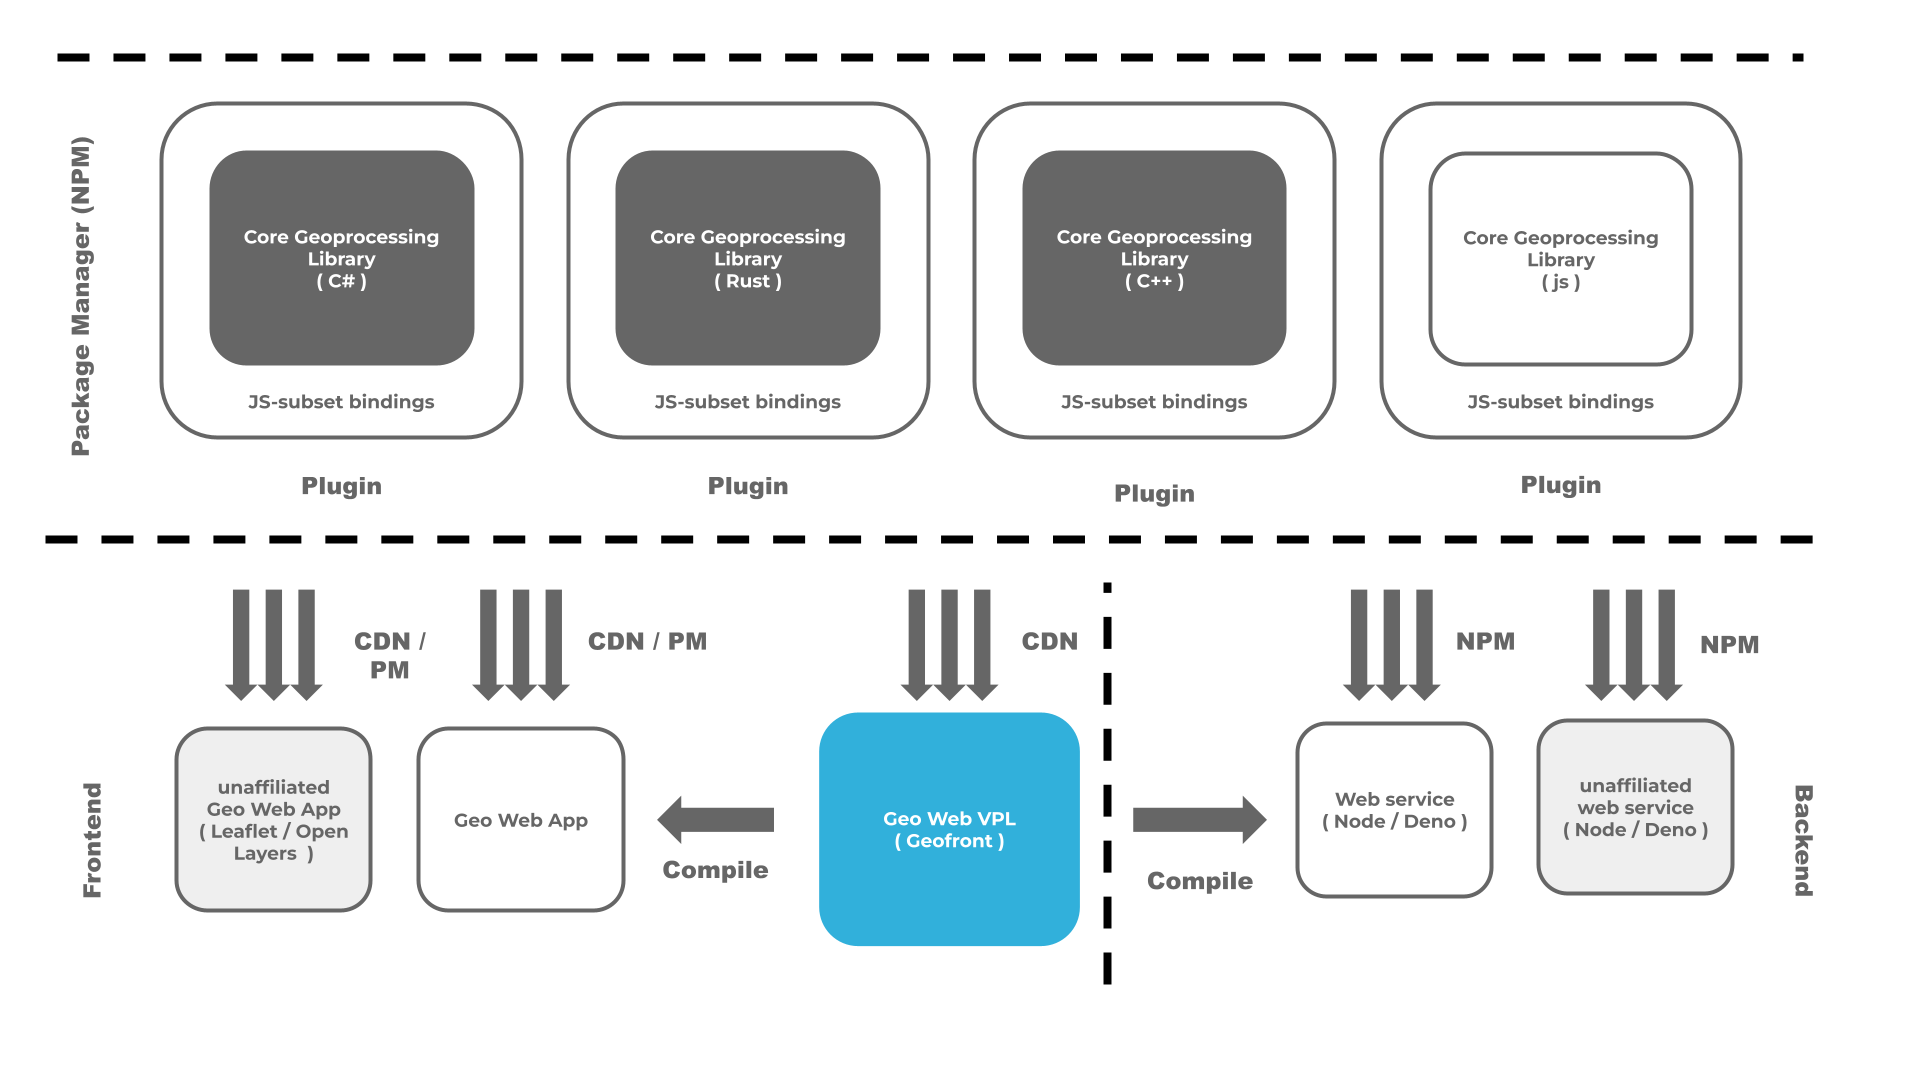
\includegraphics[width=340px]{Model Proposal.png}
  \caption{Plugin Model}
  \label{fig:plugin-model}
\end{figure}

The library model consists of two components: the design for a geo-web-vpl library, and the design for a 
loader on the side of the VPL. 
The central idea for this model is to take the wasm-wrappers created in \refsec{sec:method-two}, and to either interpret the required information from the wasm binary and related files, or, if that is impossible, add the required information in the wasm wrapper library itself.
By doing so, we make sure that at the very least, only one wrapper library is required for exposing any non-js library to the \ac{geo-web-vpl}.
The following information is required for the VPL to load a geocomputation library, and convert it into visual components:

Mandatory: 
\begin{enumerate}[-]
  \item A list of all functions present in the library, named.
  \item A list of all custom types (structs / classes) present in the library, also named.
  \item Per function:  
  \subitem A list of all input parameters, name and type.
  \subitem An output type.
\end{enumerate}

Optional: 
\begin{enumerate}[-]
  \item Per function:
  \subitem A custom name.
  \subitem A description to explain usage.

  \item Per type:
  \subitem A custom name.
  \subitem A description to explain usage.
  \subitem A definition of how to serialize and deserialize this type  
  \subitem A definition of how to render this type in 3D
  \subitem A definition of how to convert this type to basic types present within the geo-web-vpl.  
\end{enumerate}

The necessity to automate loading geocomputation libraries means that the \ac{geo-web-vpl} needs to be able to extract this information automatically. 
For scope reasons, the study limits itself to only interpret the \textbf{mandatory} information fully automatically. 
This can be achieved by using the Rust-wasm toolset "\m{wasm-bindgen}". 
\m{wasm-bindgen} is able to generate javascript wrapper bindings for a \ac{wasm} library, accompanied by TypeScript type definitions (Source). 
These are given in a 'd.ts' file, which can be understood as a header file, exposing the types required by all functions found in its corresponding javascript file. 
By including the typescript compiler in the \ac{geo-web-vpl} prototype, this header file can be loaded and interpreted to find all mandatory data, including the names and path of functions and types. 
These can then be accessed by reflecting these names and paths with the javascript files, which in turn calls the underlying \ac{wasm} binary.

The \textbf{optional} data is exposed by using 'magic methods', a strategy influenced by the python programming language (source). 
The library loader of the VPL will load certain functions, types, and methods in a special way, indicated by a naming convention. 
These functions are loaded by the vpl, but will not be converted into visual components. 
Instead, these functions are programmatically called when the VPL engine or the user requires this optional aspect. 

%%%%%%%%%%%%%%%%%%%%%%%%%%%%%%%%%%%%%%%%%%%%%%%%%%%%%%%%%%%%%%%%%%%%%%%%%%%%%%%
%%%%%%%%%%%%%%%%%%%%%%%%%%%%%%%%%%%%%%%%%%%%%%%%%%%%%%%%%%%%%%%%%%%%%%%%%%%%%%%
%%%%%%%%%%%%%%%%%%%%%%%%%%%%%%%%%%%%%%%%%%%%%%%%%%%%%%%%%%%%%%%%%%%%%%%%%%%%%%%
%%%%%%%%%%%%%%%%%%%%%%%%%%%%%%%%%%%%%%%%%%%%%%%%%%%%%%%%%%%%%%%%%%%%%%%%%%%%%%%
%%%%%%%%%%%%%%%%%%%%%%%%%%%%%%%%%%%%%%%%%%%%%%%%%%%%%%%%%%%%%%%%%%%%%%%%%%%%%%%

\section{\mySubRQFourTitle} 
\label{sec:method-four}

\begin{note}
  CUT OUT THE USE-CASE APPLICATION ASPECT. 
  -> we can make a utilization assessment based on the criteria alone, We dont need to create an application.
\end{note}

The final component of the methodology is dedicated to overcoming the fourth and final challenge to realizing a \ac{geo-web-vpl}, and involves the utilization of all aforementioned components. 
In this section, we wish to discover the practical usefulness of a \ac{geo-web-vpl}, encompassed by the research question : \mySubRQFour

% What are the advantages and disadvantages of using an existing geoprocessing library through a geo-web-vpl, as opposed to native utilization of said library?

% [WHY]
This component of the methodology is included in the study because of the following: 
It might be the case that a geo-web-vpl \emph{is} able to represented by a web-browser, and \emph{is} able to load and run functions from native, non-js geo-computation libraries. 
And still, it might not be able to successfully \emph{use} these libraries. 
The entire idea of a vpl might not be sensible for the operation at hand, or some other, unforeseen aspects mitigates the practical usefulness of the environment. 
It is therefore vital to access the actual usage of the application for accessing a geocomputation library.

% [HOW]
To answer the question of \mySubRQFourTitle, the following plan was used: 
\begin{enumerate}[-]
  \item Develop a representative use-case application within the prototype \ac{geo-web-vpl}.
  \item Develop a command line application capable of the very same process.
  \item Assess both applications according to a series of assessment questions.
\end{enumerate}

The execution of this component of the methodology is found in \refchap{chap:results-analyses}.

\subsection{use-case application}
The application used in both test cases is an "isocurves from DTM" process. 
But also: we want the iso-curves of a specific location. How to get this data is part of the exercise

\begin{note}
[This is subject to change, according to how much I can accomplish ]

- find the required height data as WFS / WMS
- determine a boundary
- load a dtm as a regular png / tiff image
- specify the parameters, like height delta, smoothness.
- marching squares
- post-process curves
- save as wkt, geojson, or some other well-known vector format


\end{note}

\subsection{Assessment Criteria}
For the assessment criteria, the cognitive dimensions framework of \cite[]{green_usability_1996} will be used. 
The framework is useful for its focus on language features. 
This allows the assessment to be made within the scope of this study, and without performing user-testing.
Also, as commented on in \refsec{sec:background-vpl}, the study has acquired a canonical nature among many VPL researchers for its elaborate examination of the "Psychology of Programming".
The age of the study indicates that the principles have stood the test of time. 

The framework presents the following 13 dimensions and accompanying descriptions \cite[]{green_usability_1996}:
\begin{enumerate}
  \item Abstraction gradient: What are the minimum and maximum levels of abstraction? Can fragments be encapsulated? 

  \item Closeness of mapping: What 'programming games' need to be learned? 
  
  \item Consistency: When some of the language has been learnt, how much of the rest can be inferred? 
  
  \item Diffuseness: How many symbols or graphic entities are required to express a meaning? 
  
  \item Error- proneness: Does the design of the notation induce 'careless mistakes'? 
  
  \item Hard mental operations: Are there places where the user needs to resort to fingers or pencilled annotation to keep track of what's happening? 
  
  \item Hidden dependencies: Is every dependency overtly indicated in both directions? Is the indication perceptual or only symbolic? 
  
  \item Premature commitment: Do programmers have to make decisions before they have the information they need? 
  
  \item Progressive evaluation: Can a partially-complete program be executed to obtain feedback on 'How am I doing'? 
  
  \item Role- expressiveness: Can the reader see how each component of a program relates to the whole? 
  
  \item Secondary notation: Can programmers use layout, colour, other cues to convey extra meaning, above and beyond the 'official' semantics of the language? 
  
  \item Viscosity: How much effort is required to perform a single change? 
  
  \item Visibility: Is every part of the code simultaneously visible (assuming a large enough display), or it it at least possible to juxtapose any two parts side-by-side at will? If the code is dispersed, is it at least possible to know in what order to read it?
\end{enumerate}

As stated by the authors; the purpose of this framework is to make the trade-offs chosen by a language's designer explicit. It is not meant as a 'scoring' system.

% Nielsen and Molichs 10 User Interface Design Guidelines
% https://theomandel.com/resources/golden-rules-of-user-interface-design/
% https://www.interaction-design.org/literature/article/user-interface-design-guidelines-10-rules-of-thumb
% (old rules, but still relevant)_


\chapter{Implementation}%%%%%%%%%%%%%%%%%%%%%%%%%%%%%%%%%%%%%%%%%%%%%% 
\label{chap:implementation}
This chapter presents the execution of the first and second step of the methodology. 
It discusses the achieved functionality, and mentions the ways this implementation fell short of the methodology.

\section{The Geofront Application}
\label{sec:implementation:app}

\begin{figure}
  \centering
  \graphicspath{ {../../assets/images/implementation/} }
  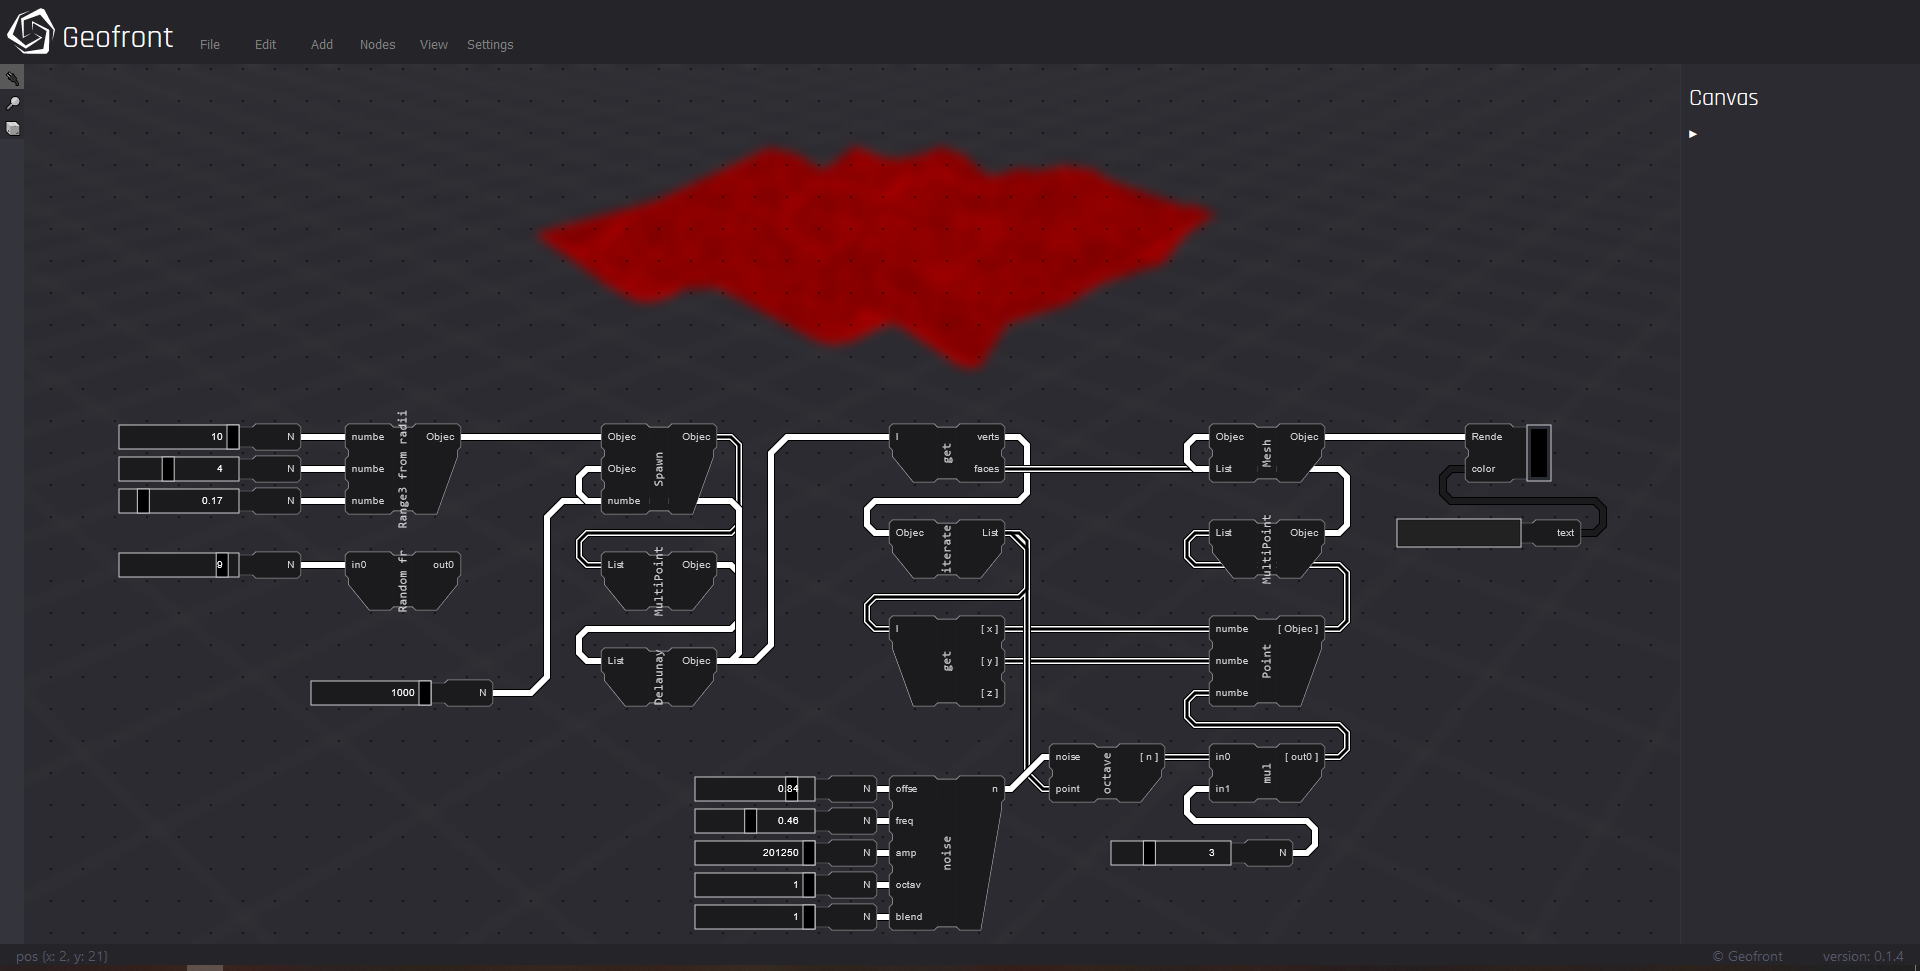
\includegraphics[width=\linewidth]{full-application.png}
  \caption[Geofront]{The Geofront Application}
  \label{fig:geofront-app}
\end{figure}

This section discusses the extend of the prototype \ac{VPL} implementation. 
The prototype is titled "Geofront", as a concatenation of "geometry" and "frontend".
Geofront exists as a set of loosely coupled repositories, all published on the version control platform GitHub under the MIT license. These repositories are grouped under the GitHub Organization \m{thegeofront} .

% TODO: do something with appendix
% (SOURCE: https://github.com/thegeofront)

The Geofront Application is implemented according to the design layed out in \refsec{sec:method:base-vpl}, and uses TypeScript as its main language. 
\m{webpack} is used to compile this codebase into a singular javascript file, and this file practically serves as the full application. 
the repository spend around 9.000 lines of code, divided into core categories and functionalities.
What follows is a clarification of the implementation of some of these categories.

\subsection{Model}

The visual programming language model as described by \refsec{sec:method-model} could be fully implemented on the web. 
Both the shims as well as the model itself was implemented in typescript, and no special web features were utilized in the creation, despite HashMaps and HashSets offered by the Typescript language. 
This model allows Geofront to internally represent the data structure and logic of a dataflow-VPL program. 
The programs constructed with the VPLs are dubbed 'scripts'.

Type safety was fully implemented by essentially creating a new 'layer' of types on top of typescript \reffig{fig:geofront-types}.
The type system can be extended by types found in Geofront Plugins.  
In theory, this can be used to prevent all incorrect type usage during creation of a Geofront graph, and before calculation.
In practice, to support iteration, some runtime type checking was still required. 

\begin{figure}
  \centering
  \graphicspath{ {../../assets/images/implementation/} }
  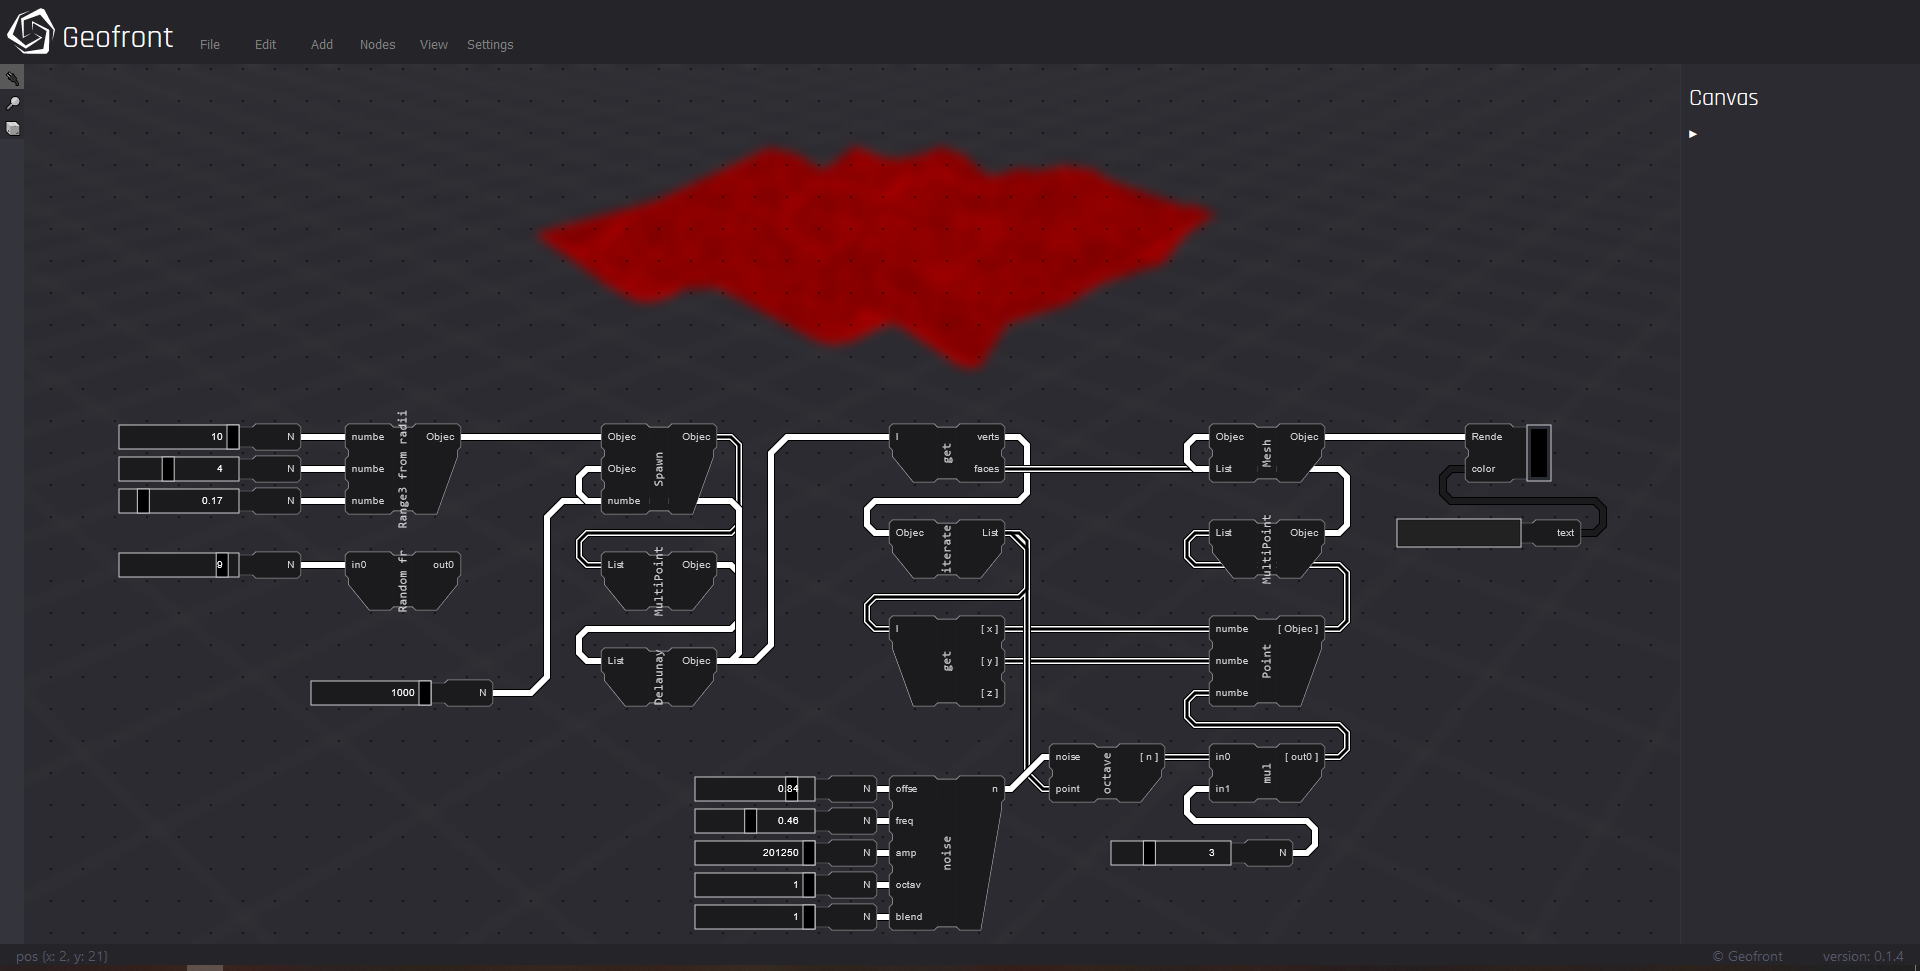
\includegraphics[width=\linewidth]{full-application.png}
  \caption[Geofront]{The Geofront Application}
  \label{fig:geofront-types}
\end{figure}

\subsection{View}

\subsubsection{The graph}

\begin{figure}
  \centering
  \begin{subfigure}[b]{0.30\linewidth}
    \graphicspath{ {../../assets/images/implementation/} }
    \centering
    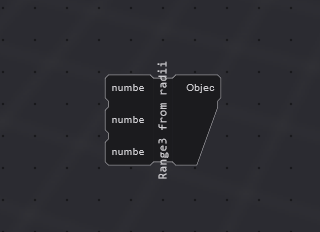
\includegraphics[width=\linewidth]{node.png}
    \caption{}\label{fig:node-cable:1}
  \end{subfigure}%
  \qquad 
  \begin{subfigure}[b]{0.30\linewidth}
    \graphicspath{ {../../assets/images/implementation/} }
    \centering
    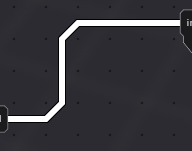
\includegraphics[width=\linewidth]{cable.png}
    \caption{}\label{fig:node-cable:2}
  \end{subfigure}%
  \qquad 
  \begin{subfigure}[b]{0.30\linewidth}
    \graphicspath{ {../../assets/images/implementation/} }
    \centering
    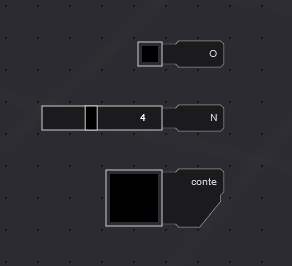
\includegraphics[width=\linewidth]{widgets.png}
    \caption{}\label{fig:node-cable:3}
  \end{subfigure}%
  \caption[Nodes, Widgets and Cables]{The basic canvas components of Geofront: a Node (A), a Cable (B), and some Widgets (C) }
  \label{fig:node-cable}
\end{figure}

The graph data model must be rendered to the screen so users can comprehend and edit the graph. 
This visualization is achieved by using the HTML5 Canvas Api. 
The Canvas API is a raster-based drawing tool, offering an easy to use, high-level api to draw 2D shapes such as lines, squares, circles, and polygons. 
The Nodes Canvas uses this API to draw polylines and polygons at runtime, to represent the cables and nodes respectively. 
These basic shapes and their styles change dynamically, based on features like the length of a cable, how many input sockets a node requires, or whether or not a node is selected. 

Like other HTML5 features, the main advantage is that this API is included and implemented within the browser itself. This method is fast thanks to its C++ based implementation, and can be used without the need to include anything within the source code of the application.

The downside of this implementation, is that all features the HTML renderer normally accounts for, like picking, conditional styling, and performant rendering of repetitious elements, are lost.
These had to be re-implemented in typescript, which will never be as performant as the codebase of the browser engines themselves. 
An additional limitation is that the draw calls are primarily CPU based, 
making it less performant than a WebGL \& glsl implementation would have been.
lastly, the implementation chose to redraw the full canvas on every registered change to the graph, instead of partial redraws. 

These limitations come together to a performance linear to the amount of nodes and cables drawn. For the current implementation and scale of Geofront, this performance is acceptable.  
Still, the application slows down when rendering a large amount of components (See TODO). 

\begin{note}
  TODO Show a graph with performance considerations
\end{note}

This performance hit is partially due to the implementation, and partially due to browser feature limitations. 
The browser does not offer a 'middle ground' between html-like rendering and 2D canvas-like rendering required for a visualization like the dataflow graph. 
Still, this implementation could have experimented more with a HTML + SVG based render method.

\subsubsection*{Presentation}

\begin{figure}
  \centering
  \graphicspath{ {../../assets/images/implementation/} }
  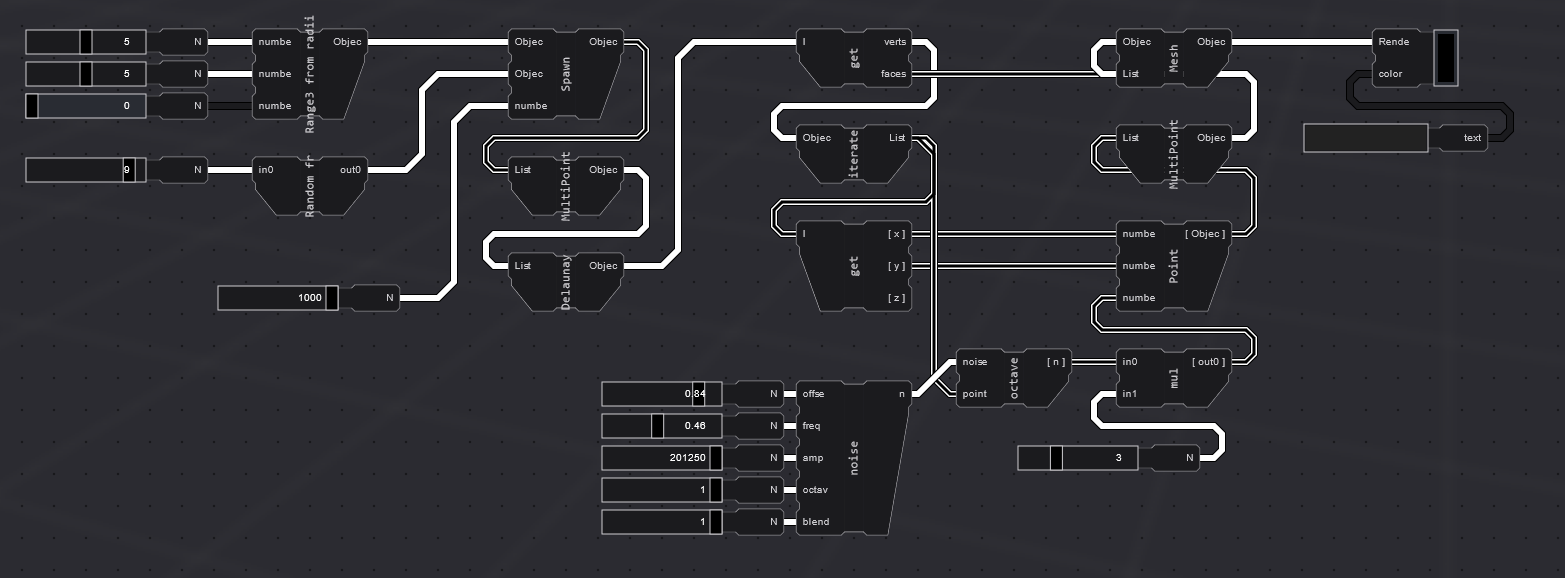
\includegraphics[width=\linewidth]{a-full-graph.png}
  \caption[Shim Classes]{A complete Geofront script}
  \label{fig:a-full-graph}
\end{figure}

Special care has been put into the presentation of the implementation.
The layout takes inspiration from various geometry VPLs mentioned at \refsec{sec:related-geovpl}, such as Blender's GeometryNodes, McNeel's Grasshopper, and Ravi Peter's GeoFlow. 
A few notable exceptions, however. 
Firstly, the entire graph is placed on a grid, and all nodes adhere to this grid (see \reffig{fig:a-full-graph}). 
For example, a node with three inputs will always occupy three grid cells in height. 
This grid is applied for much of the same reason as terminals \& source code are displayed using monospaced fonts. 
Consistent sizing encourages organization and clarity, for this makes it easy for components to line up, and predict how much space something requires.  
Cables also adhere to the grid. They alter their shape in such a way to remain as octagonal as possible, in an attempt to make connections between nodes more readable.
% This takes some additional inspiration from subway maps, as well as the design of computer chips. 
% This makes for a good fit, as these spatial configurations and the Geofront Script are all focussed on organizing connectivity.

\subsubsection*{3D Viewer}

\begin{figure}
  \centering
  \graphicspath{ {../../assets/images/implementation/} }
  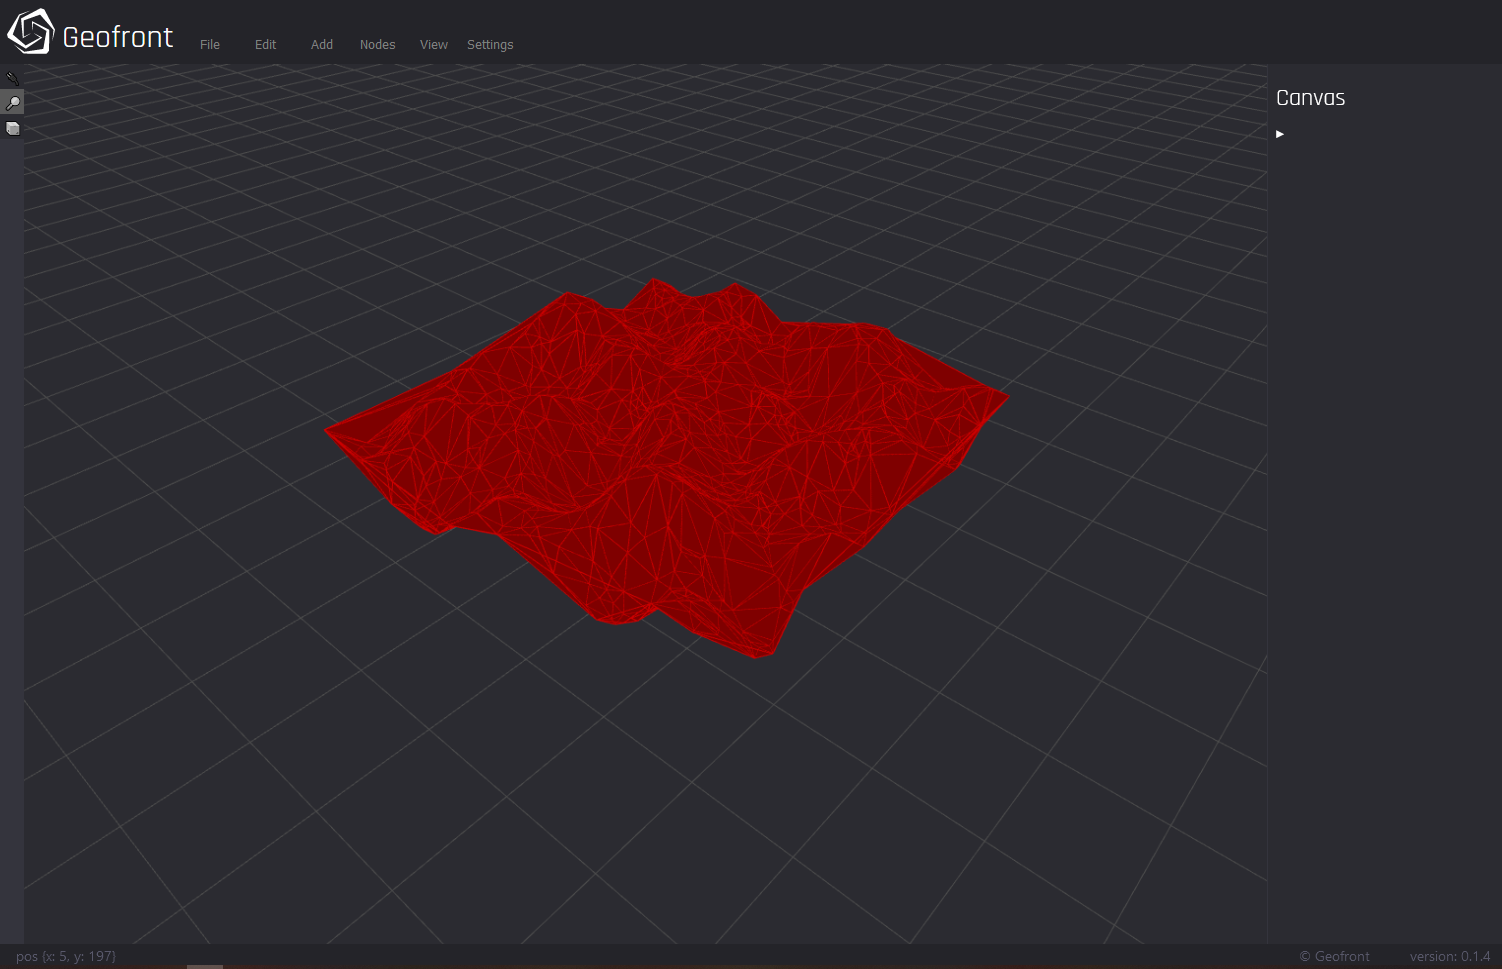
\includegraphics[width=\linewidth]{viewer.png}
  \caption[Geofront viewer]{The Geofront Viewer}
  \label{fig:geofront-viewer}
\end{figure}

The 3D viewer attached to the geofront application is also implemented in typescript. 
It uses WebGL and the OpenGL Shading Language (glsl) as its graphics API. 
The viewer can be used to represent and visualize various geometries, such as points, lines, meshes, bezier curves, and bezier surfaces.
Images can also be rendered, which are represented as a quad mesh with a texture. 

The useful aspect of WebGL is the fact it does not have to be included within the source code of a program. 
WebGL supports all render demands basic, small-scale 3D geodata visualization might need, such as point clouds and DTMs.
large scale visualization is not possible, as the visualizer does not support idioms like frustum culling, or dynamic levels of detail. 
Additionally, the viewer does not support

These visualization options open the possibility of visualizing a great number of different geodata types, such as DTM / DSM, GEOtiff, Point clouds, and OGC vector data. 
However, specific visualization convertors are not implemented, for these are reliant upon the compilation of existing geocomputation libraries. 

\begin{figure}
  \centering
  \begin{subfigure}[b]{0.45\linewidth}
    \graphicspath{ {../../assets/images/implementation/} }
    \centering
    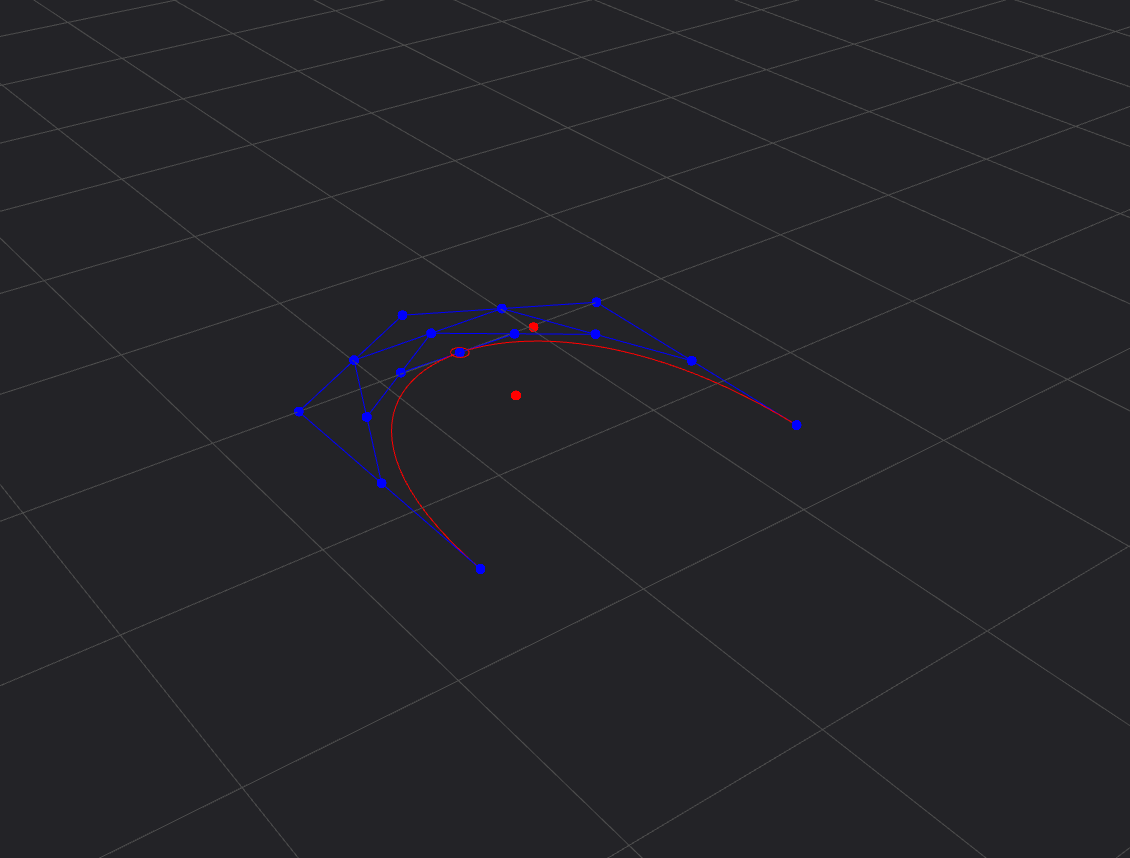
\includegraphics[width=\linewidth]{viewer-2.png}
    \caption{}\label{fig:viewer-geometries:1}
  \end{subfigure}%
  \qquad 
  \begin{subfigure}[b]{0.45\linewidth}
    \graphicspath{ {../../assets/images/implementation/} }
    \centering
    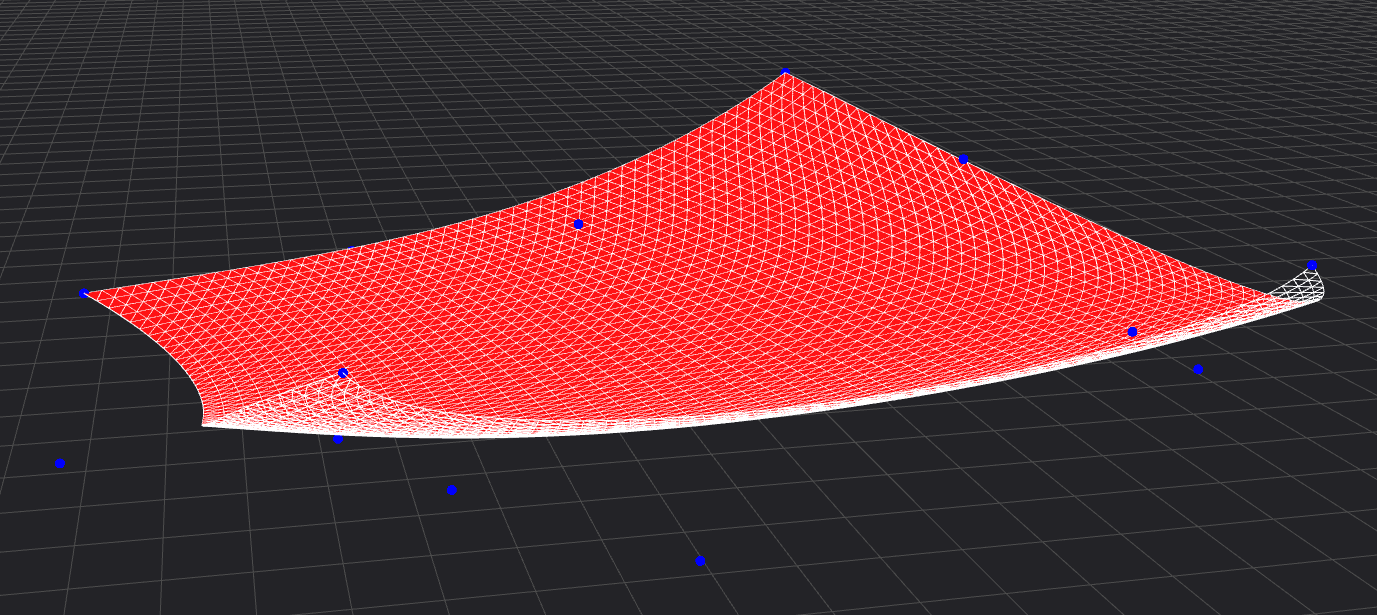
\includegraphics[width=\linewidth]{viewer-3.png}
    \caption{}\label{fig:viewer-geometries:2}
  \end{subfigure}%
  \caption[Geofront viewer geometries]{A bezier curve and surface visualized using the geofront viewer}
  \label{fig:viewer-geometries}
\end{figure}

\subsection{Controller}

% \item an interface to create and edit this graph 
% \item a way to provide input data 
% \item a way to execute the language
% \item a way to display or save output data

\subsubsection*{Calculation}
Execution of the graph is implemented as described by the methodology, albeit with a major setback: execution does not run on a separate thread. 
This means that the interface freezes up during large calculations.

The reason for this is the difficulty in achieving concurrency in the browser. 
Web workers have to be implemented and instantiated using separate javascript files. 
Not only is this unusual, it forces a codebase to create separate files per multithreaded operation.
The dynamic nature in which some of Geofront dependencies are loaded made splitting up the codebase like this difficult, let alone using multiple threads for calculating each node.

\subsubsection{Interaction}
User Interaction is made possible through the \href{https://developer.mozilla.org/en-US/docs/web/api/event}{HTML DOM Events}. 
This api provides ways to listen to many events, including keyboard and mouse events. 
When the mouse is moved, its screen-space position is transformed to a grid position, which allows the user to select one or multiple objects. 

Geofront's user interface strives to match features of regular desktop applications. 
As such, the Geofront Graph supports features like undoing, redoing, duplication, copying, and pasting. 
These functionalities can be used with the expected keyboard combinations (Ctrl + C / Ctrl + V).
However, the implementation does lack touch \& mobile support.

In general, these editing features are complete, but there are a few caveats caused by the browser environment.
Namely, the browser has need of its own controls and shortcuts. 
For example, the right mouse button brings up the browser context, and the \m{Ctrl + W} shortcut closes a browser tab, which cannot be overwritten.
While there are some workarounds, these aspects make web applications more 'convoluted' to implement than would otherwise be ideal.

\subsubsection*{Input and Output}
The base dataflow VPl component of Geofront support input and output UI elements, like sliders, buttons, and text fields.
These form special nodes on the canvas, called 'widgets'. 
Widgets simply are nodes with side effects. 
By making this a different type of node, the behavior of the graph becomes more predictable.

The fact that the Geofront implementation opted for a canvas API-based visualization made it so HTML could not be used for these aspects, and all these features had to be created within the constraints of the Canvas API.

Files can be used as inputs and extracted as outputs using the 'file load' and 'file save' widgets. 
These files are then loaded as raw text or raw binary, which can be parsed by using a parser appropriate for that file type. 
The problem with this implementation, is that it requires a full file to be loaded into memory. 
Most native parsers make use of streaming to avoid this. 
There are ways of supporting incrementally reading files in a browser, but these methods are not supported by all browsers yet. 

%%%%%%%%%%%%%%%%%%%%%%%%%%%%%%%%%%%%%%%%%%%%%%%%%%%
%%%%%%%%%%%%%%%%%%%%%%%%%%%%%%%%%%%%%%%%%%%%%%%%%%%
%%%%%%%%%%%%%%%%%%%%%%%%%%%%%%%%%%%%%%%%%%%%%%%%%%%


\newpage
\section{The plugin system}
\label{sec:implementation:loading}

The plugin system is implemented according to design discussed in \refsec{sec:method:plugin-system}.
The implementation comes down to a plugin loader written inside of the Geofront application, with an accompanied workflow of how to create such a plugin. 

\subsection{The plugin loader}
\label{sec:implementation:loading:limits}

The plugin loader implemented in Geofront can load a javascript / typescript library, and convert it into appropriate visual components. 
What this looks like in practice can be seen in \reffig{fig:todo-1}.
As prescribed by the methodology, Typescript declaration files are loaded to determine the name, location, parameter types of functions. 
This works similar for libraries which include a WebAssembly binary.

While in theory any javascript / typescript library can be used, in practice some limitations are in place due to the specific implementation used:

\subsubsection*{Files}
Firstly, the current loader accepts only one Javascript file, and one Typescript Declaration file per library.
A library without a 'd.ts' declaration cannot be used. 
If additional files are used, such as \ac{wasm} files, these will have to be explicitly fetched and run by the javascript file. 
For the purposes of this study this is acceptable, as the used \ac{wasm} compilers work in a manner compatible to these limitations.
Javascript bundlers also help to adhere to these limitations.
Still, this does mean that not just any javascript library can be imported. 

\subsubsection*{Library Structure}
Secondly, while the loader does support namespaces and classes, not all types of libraries and programming styles are supported. 
Functions using callbacks, promises, complex types, or generics, cannot be properly loaded. 
Libraries utilizing "method chaining APIs" can be loaded, but are difficult to use as intended on the Geofront Canvas.
Also bear in mind that the loader does not perform any checks to see if the loaded library actually uses pure functions. 

\begin{note}
  TODO show example
\end{note}

\subsubsection*{Types}
The plugin loader can only load functions using acceptable input and output types. 
Not all input and output arguments translate well to the format of a dataflow VPL. 
The types may only include: 
\begin{itemize}
  \item basic javascript types (boolean / number / string)
  \item basic jsons (unnamed structs), objects, interfaces 
  \item javascript ArrayBuffers like \m{Float32Array} (vital for performant data transfer)
\end{itemize}
The typesystem of the plugin loader will pick up on types exposed by a library, and include them within the type safety system of Geofront. 
However, this does mean that certain types are not supported, like asynchronous promises, or functions as variables. 

\begin{figure}
  \centering
  \graphicspath{ {../../assets/diagrams/} }
  % 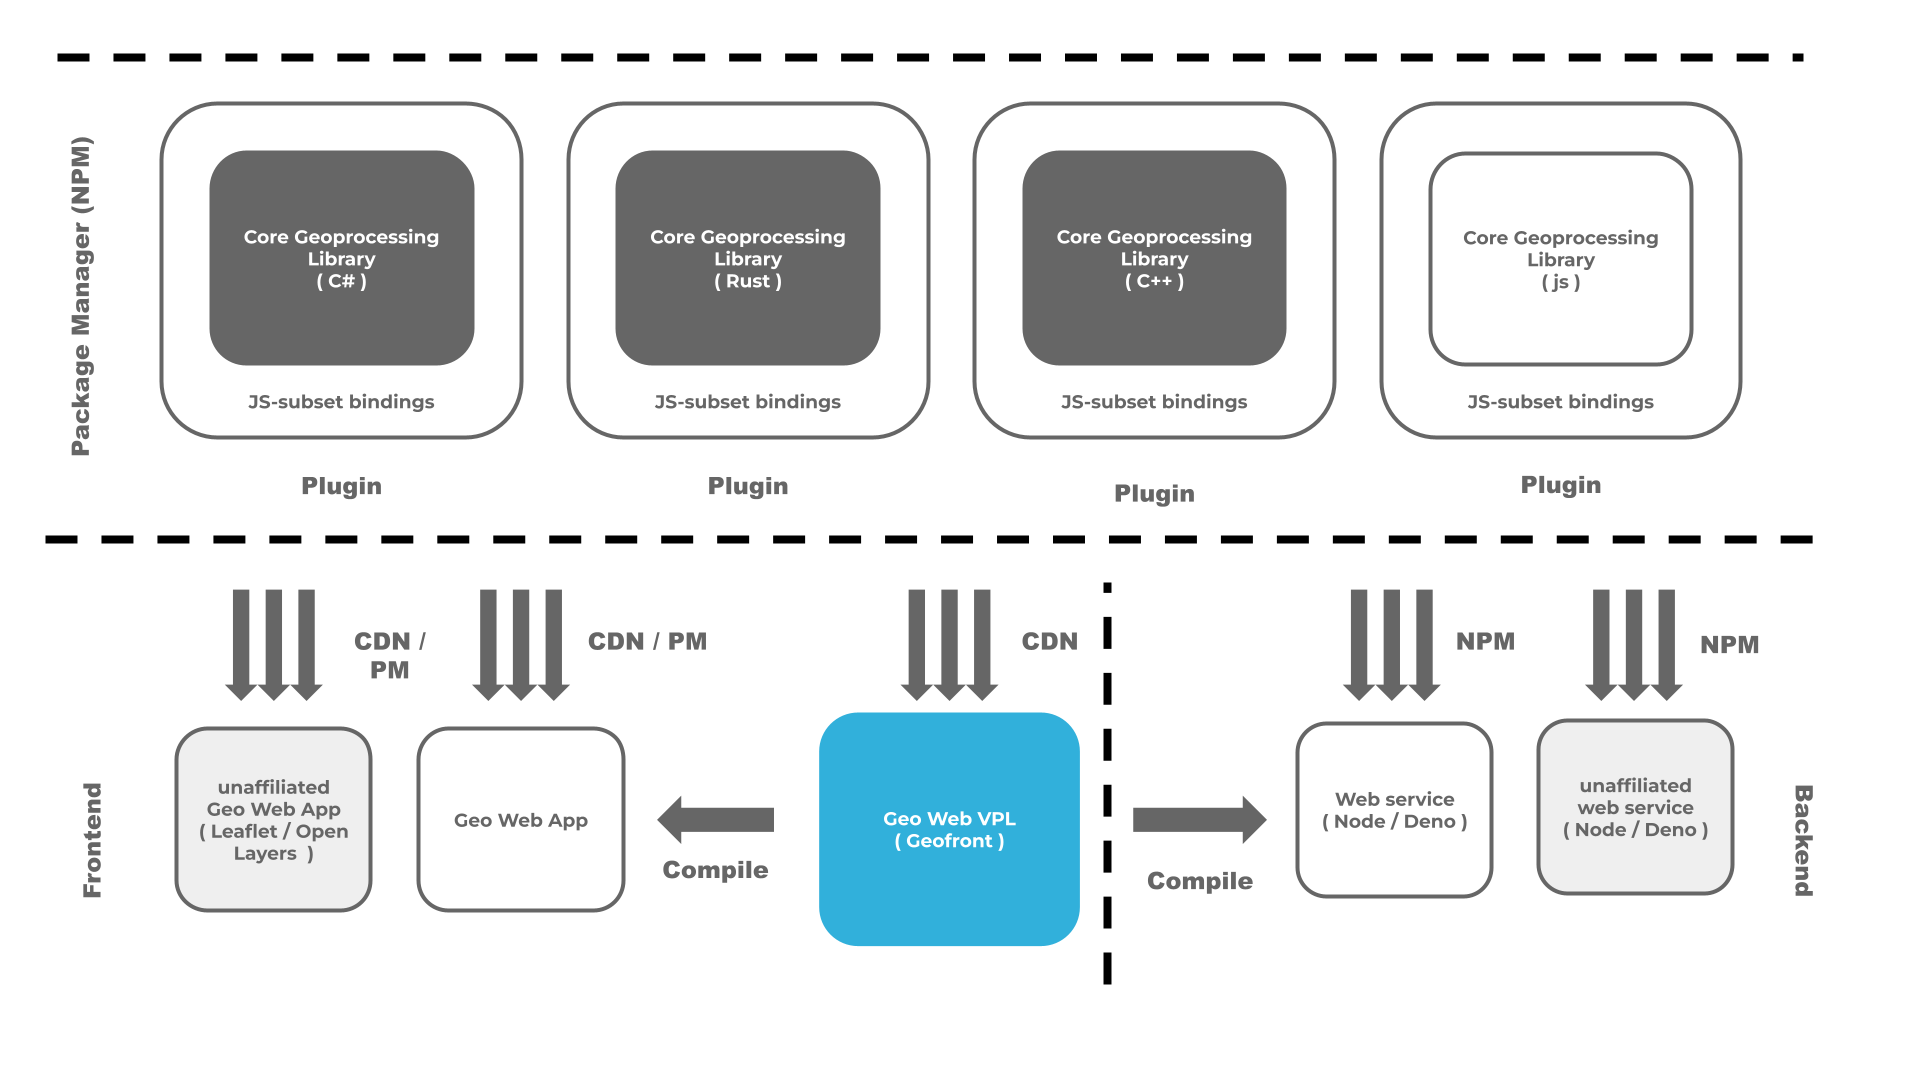
\includegraphics[width=\linewidth]{Model Proposal.png}
  \caption[]{TODO: show importer side-by-side}
  \label{fig:todo-1}
\end{figure}


\begin{figure}
  \centering
  \graphicspath{ {../../assets/diagrams/} }
  % 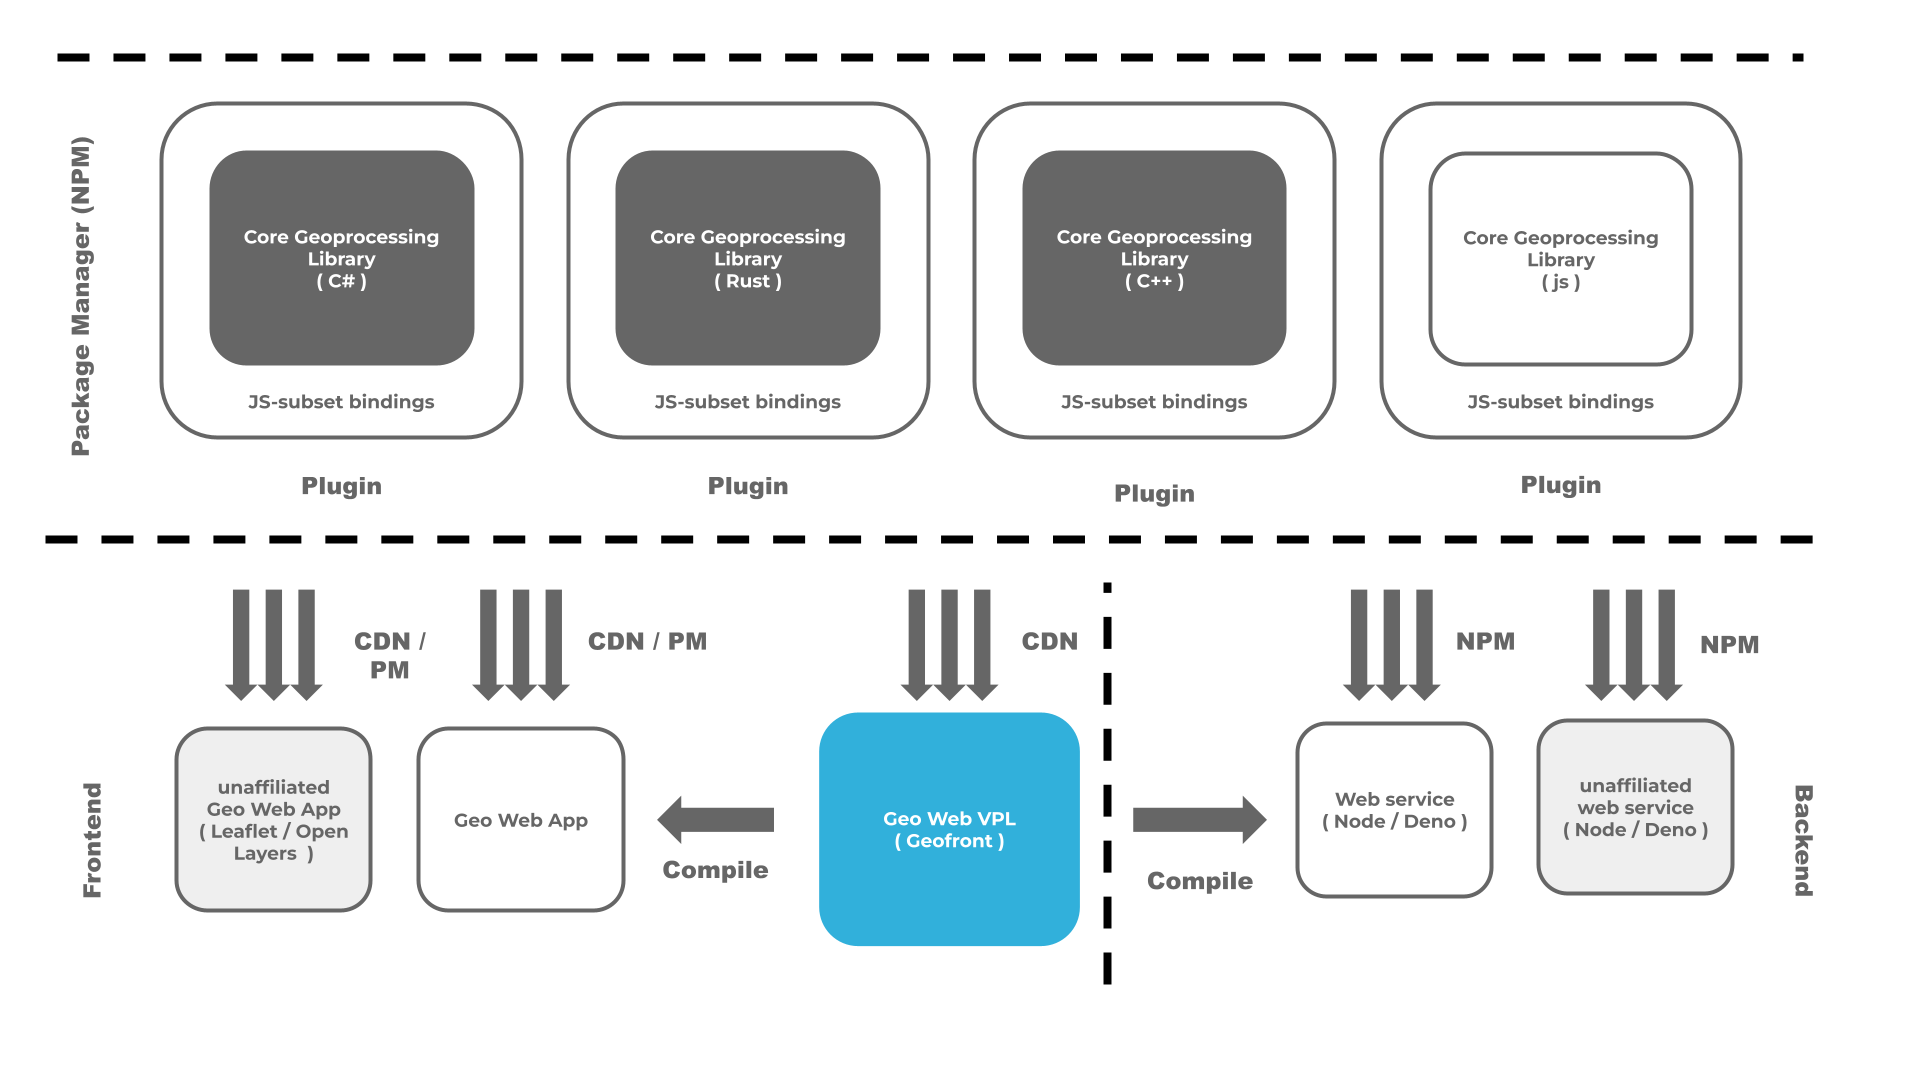
\includegraphics[width=\linewidth]{Model Proposal.png}
  \caption[]{TODO: show more achieved functionality}
  \label{fig:todo-2}
\end{figure}

\subsubsection*{Supported languages}
Finally, not all languages are equally supported:

\begin{itemize}[-]
  \item \textbf{Javascript / Typescript}: 
    If the Javascript and Typescript files used adhere to the limitations mentioned above, the library can be used. 
    However, a bundler needs to be used to include all sub-dependencies of a library, as the Geofront loader does not load sub-dependencies currently. 

  \item \textbf{Rust}:
    Libraries compiled to webassembly using the "\m{wasm-bindgen}" work "out of the box" in most cases.
    \m{wasm-bindgen} is able to generate javascript wrapper bindings for a \ac{wasm} library, accompanied by TypeScript type definitions. 
    This wrapper handles type conversions. 
    
    However, rust libraries compiled to the web do require a initialization step. 
    As such, the loader now checks if the library looks like a Rust library, and if it does, it uses a slightly altered loading method.
  \item \textbf{C++}
    At the time of writing this study, the 'embind' compiler (explained in \refsec{sec:implementation:loading}) does not have an option to compile a typescript declaration file. 
    Additionally, the javascript generated to wrap the wasm binary is not a wrapper handling type conversions and memory safety like Rust. 
    Instead, it uses a custom architecture programmatically expose javascript wrapper functions one by one, and leaves it to the user of the library to deal with type conversions and memory safety. 
    
    These two aspects combined makes it so C++ cannot use Geofront's loader directly, and must use an additional in-between wrapper libraries.

  \item \textbf{Other languages}
    This study only experimented with Rust and C++ as non-js languages.
    While the loader's ability to work with WebAssembly is promising, additional testing is required before Geofront can claim to support any language. 
\end{itemize}

\subsection{Achieved Workflow}
% \emph{show the insane (rust + wasm + npm) workflow}

With all the above considerations in mind, the following workflow can now be used to create a Geofront Plugin, which, as explained, doubles as a normal javascript library. 
If Rust or C++ is used, this setup in a way triples as also a native geoprocessing library.
The Geofront standard library is also implemented by using workflow with Rust.

\begin{lstlisting}
  
  Using Typescript: 
  1. Write or find a geoprocessing / analysis library using typescript, 
  2. Compile and bundle to a `d.ts` + `.js` file.
  3. publish to npm 

  Using Rust: 
  1. Write or find a geoprocessing / analysis library using rust
  2. Create a second library, which exposes a subset of this 
     library as 'functions usable on the web', using 'wasm-pack'.
  3. Compile to `.wasm` + `d.ts` + `.js`.
  4. publish to npm (`wasm-pack publish`)
  
  Using C++: 
  1. Write or find a C++ based geoprocessing / analysis library. 
  2. Create a second library, which exposes a subset of this 
     library as 'functions usable on the web', using 'emscripten'*.
  3. Compile to a `.wasm` and `.js` file using emscripten.
  4. Create a third 'js' library, which wraps the functionality* 
     exposed by empscripten
  5. Manually create a corresponding `d.ts` file
  6. Publish these to npm 

  ---------------------------------------------------------

  In Geofront: 
  4. Reference the CDN (content delivery network) address of this node package. 
  5. Use the library.

  * these parts contain many caveats, explained in Section 5.2

\end{lstlisting}

\begin{figure}
  \centering
  \graphicspath{ {../../assets/diagrams/} }
  % 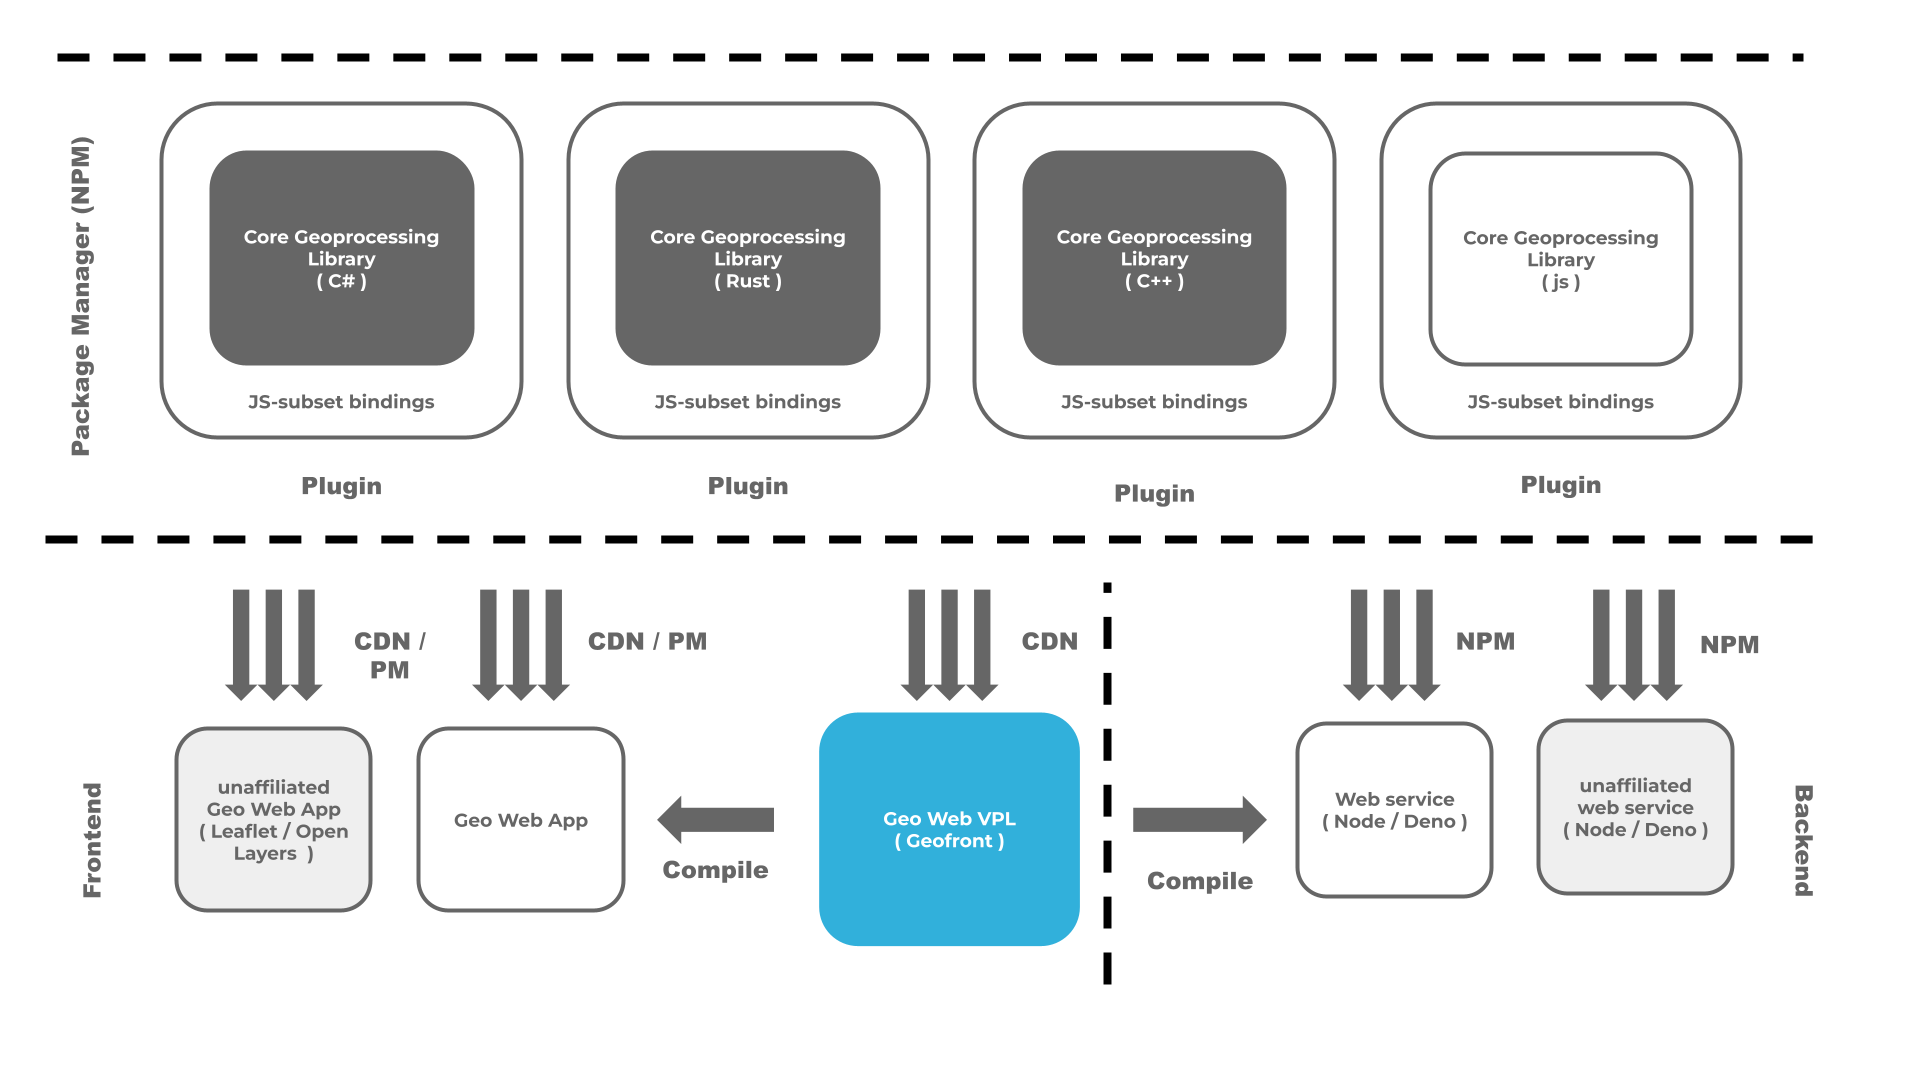
\includegraphics[width=\linewidth]{Model Proposal.png}
  \caption[]{TODO: show the achieved workflow visually}
  \label{fig:todo-more-images}
\end{figure}

\subsection{Automation and portability}

The \refsec{sec:method:plugin-system} mentioned the requirements of library portability and automation. 
In this section we assess to what extend this implementation was able to succeed on delivering these two requirements. 

\subsubsection*{Automation \& exposure of metadata}

Based on the results, we can state that the loader mitigates the need for explicit configuration only for the required, mandatory aspects. 
All optional properties like human-readable names and descriptions, must be specified explicitly using a naming convention specific to Geofront. 

In practice, however, there are some more "configuration" requirements. 
The limitations outlined by \refsec{sec:implementation:loading:limits} show that there are quite a few additional considerations. 
Geofront does not support all types or all library structures, and certain languages require additional compile limitations.

Also, while the optional properties are just that, optional, one could argue that some of these properties are in fact required. 
Libraries without 'human-readable' names and descriptions are harder to utilize in a Geofront script by end users.
While regular programming languages also allow the creation and publication of undocumented libraries, one can question if this should also be allowed for the more end-user focussed VPL libraries.

So, while the plugin loader can load some simple textual programming libraries almost without any special configuration, sizable libraries intended for consumption by Geofront will still need to be explicitly configured for Geofront.
However, even with these requirements, this can still be considered an improvement compared to the plugin systems of geometry VPLS studied at \refsec{sec:related-geovpl}, 
in which developers are required to create a class per exposed function.

\subsubsection{Portability}

This system creates seamless interoperability between a textual programming library, and a VPL plugin to an extend. 
However, because of the reasons outlined above, it is also safe to say that this seamless interoperability is only one-directional: 
Libraries intended for consumption by Geofront double as also a 'normal' javascript library. 
The configuration demands of Geofront only impair the normal, javascript-based usage by forcing a functional style, and by including certain methods only intended for Geofront. 
Even these Geofront-specific methods might prove useful in certain scenarios, such as by providing a way to visualize data.

This seamless interoperability is less prominent in the opposite direction. 
A normal javascript library, or a javascript library using WebAssembly, can't be automatically used by Geofront in most cases. 
Most libraries use an imperative programming style, use unsupported types, or consist of multiple files.
In some cases, a library is be able to be loaded, but is then functionality impaired by the interface. 

% \begin{figure}
%   \centering
%   \graphicspath{ {../../assets/images/4/} }
%   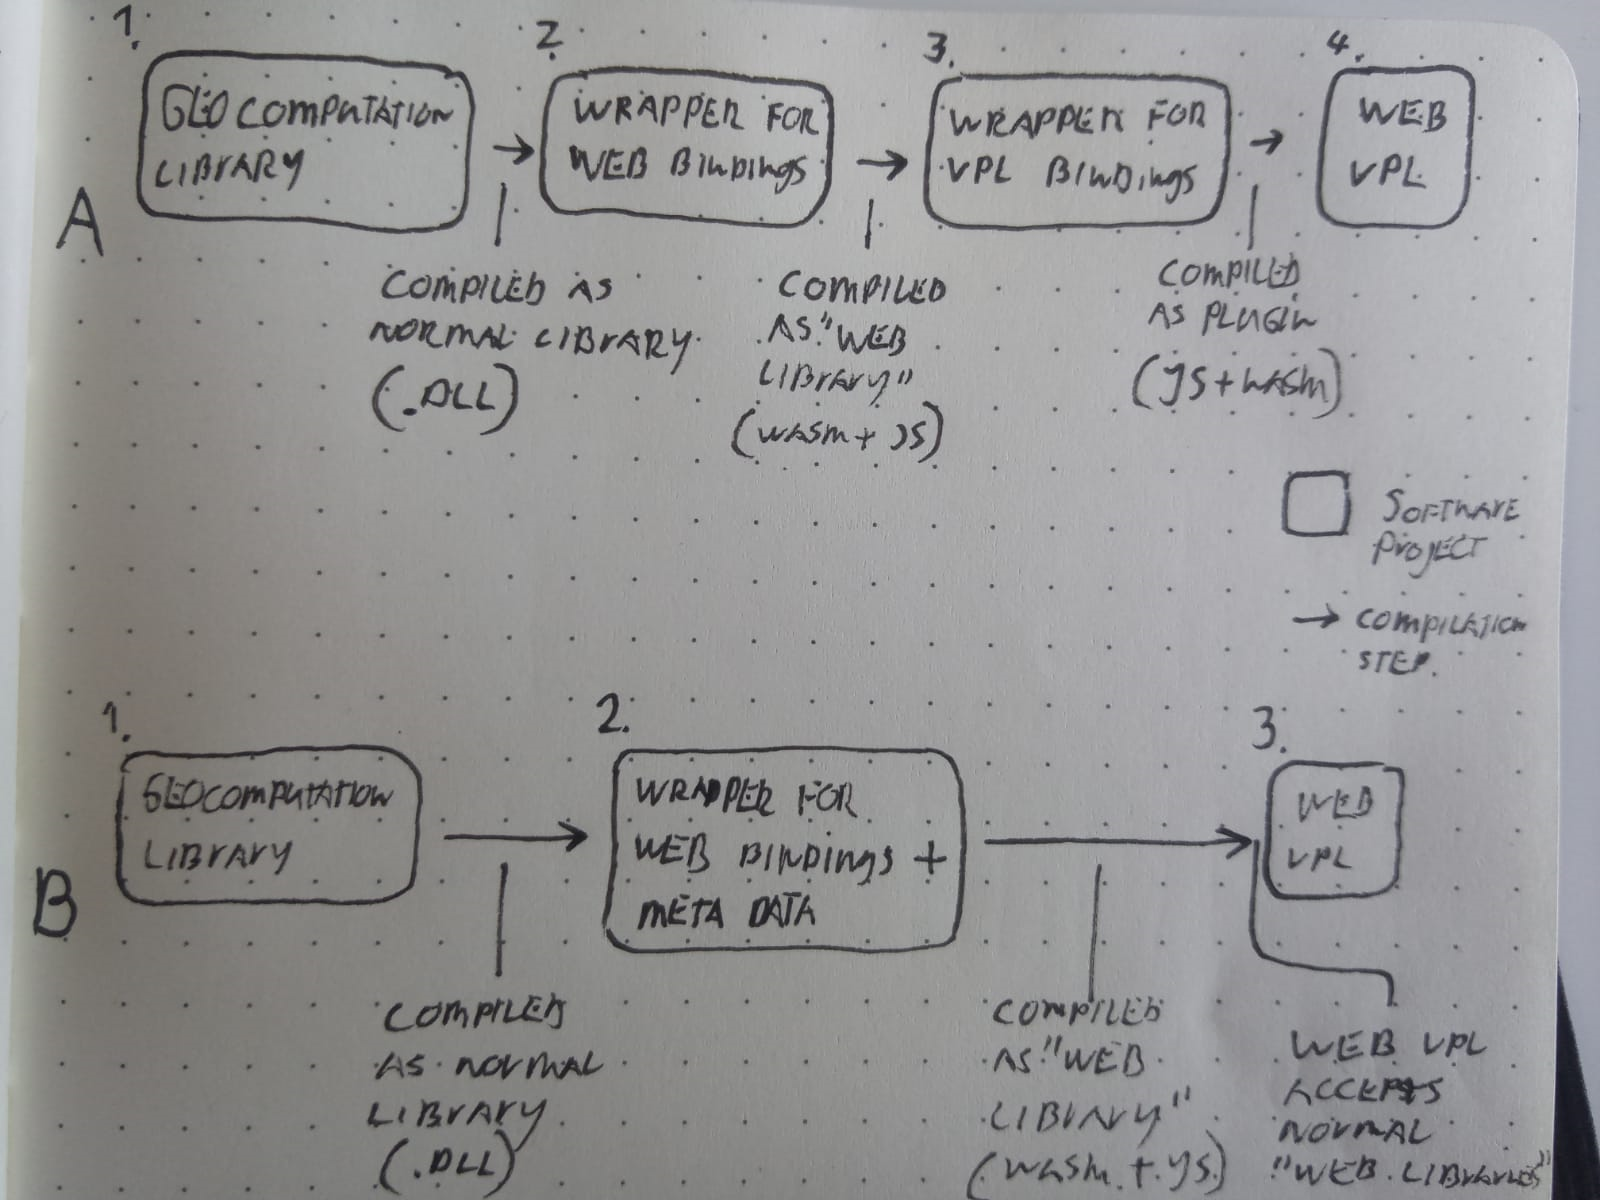
\includegraphics[width=\linewidth]{loading-trajectory.png}
%   \caption[Loading Trajectory]{Loading Trajectories}
%   \label{fig:loading-trajectory}
% \end{figure}

% \begin{note}

  % THIS IS AN ARGUMENT WHICH CAN BE USED TO DEFEND THE EFFORT TOWARDS AUTOMATION AND PORTABILITY

%   This turned out to be a problem during preliminary studies.
%   If a \ac{geo-web-vpl} wishes to use non-js libraries, it would mean that these libraries would have to be wrapped twice (see \reffig{fig:loading-trajectory} A): 
%   Once to expose the native library to the web using the methods described at \refsec{sec:method-two},
%   And once more to map the web library to the visual language. 
%   While this is a possibility, in practice, two layers of wrappers are not acceptable in terms of a development workflow.
%   This would be cumbersome, prone to errors, and hurting version control by having to synchronize between 4 software projects. 
  
%   There is also a second reason for critically addressing the way plugins are loaded. 
%   An observation was made from studying the existing geo-vpls in \refsec{sec:related-geovpl}:
%   It seems that if a developer wants to create custom VPL components, they are required to write plugins very specific to that particular VPL.
%   This means that practically, the library ecosystem of a VPL is entirely its own: 
%   It is separated from the wider context of textual programming libraries. 
%   End users are at the mercy of developers implementing their libraries in the dialect their particular VPL.
%   Meanwhile, developers are forced to implement and support a multitude of wrapper libraries for VPL platforms.  
  
%   In contrast, if the library loader of a VPL was able to directly utilize textual libraries, the barrier between vpl ecosystems and regular text-based libraries would cease to exist, benefiting both developers and end users. 
%   It might even lower the barrier between visual and textual programming in general, making it easier for VPl end-users to adopt some forms of textual programming, and vice versa. 
  
% \end{note}

\chapter{Testing}%%%%%%%%%%%%%%%%%%%%%%%%%%%%%%%%%%%%%%%%%%%%%% 
\label{chap:testing}

In this chapter the various software implementations and design choices made in \refchap{chap:implementation} are used and tested on various aspects. 
This is done to gather the data needed to answer the second, third and fourth research question. 
It consists of the sections \refsec{sec:testing:compilation} and \refsec{sec:testing:usability}.


\section{Plugin Compilation \& Utilization}
\label{sec:testing:compilation}

\subsection{Rust: minimal plugin}
The compilation of a minimum Rust plugin, exposing a function, a class, and a method was successful. 
% APPENDIX?
\reffig{fig:min-rust-plugin-code:1} Shows the source code of this plugin. 
The 'wasm-bindgen' library allows functions and classes to be annotated as 'bound to javascript'. 
This simplifies the compilation process to WebAssembly greatly. 
It also clearly states errors if a property or class are incompatible to be exposed. 

This library was compiled to WebAssembly and javascript using 'wasm-pack'. 
This produces multiple artifacts, showcased in \reffig{fig:rust-plugin:compilation-results}. 
This figure also showcases how wasm-pack wraps the functionality: 
The \m{point\_distance} function exposed by the wasm file is wrapped by the javascript file, converting it to look like a regular javascript class.

To check if the result is valid, a small html demo was created to load and use the library (see \reffig{fig:min-rust-plugin-code:2}).
Note how the JavaScript library wrapping the wasm file looks and works almost like a normal javascript library, the only difference being a 'init' function, which is required to be run before using the library, and the need to free the memory of used object with the \m{free\(\)} method.



\begin{figure}
  \centering
  \begin{subfigure}[b]{0.45\linewidth}
    \graphicspath{{../../assets/images/6.1.1/}}
    \centering
    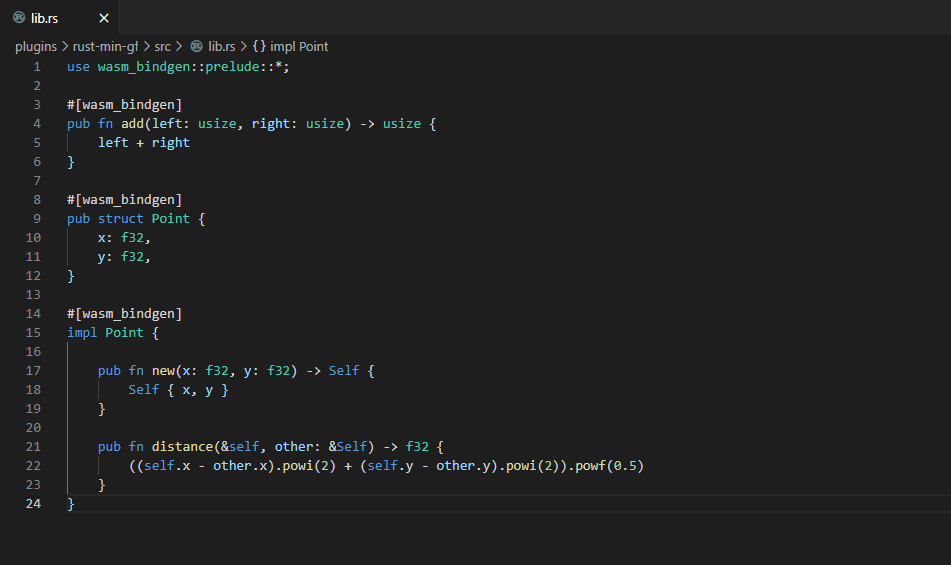
\includegraphics[width=\linewidth]{8.PNG}
    \caption{}\label{fig:min-rust-plugin-code:1}
  \end{subfigure}%
  \qquad %-- that adds some space between th 2 figures
  \begin{subfigure}[b]{0.45\linewidth}
    \graphicspath{{../../assets/images/6.1.1/}}
    \centering
    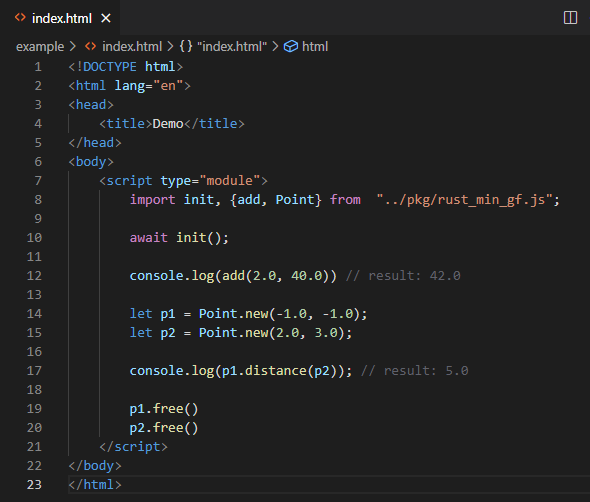
\includegraphics[width=\linewidth]{9.PNG}
    \caption{}\label{fig:min-rust-plugin-code:2}
  \end{subfigure}%

  \begin{subfigure}[b]{0.45\linewidth}
    \begin{lstlisting}
      // todo fill this with the source instead of these nasty screenshots
      function multiply(a: f32, b: f32) -> f32 {
        a * b
      }
    \end{lstlisting}  
  \end{subfigure}%

    

  \caption[minimal rust geofront plugin: usage]{Rust Source code (a) and web demo (b)}
  \label{fig:min-rust-plugin-code}
\end{figure}

\begin{figure}
  \graphicspath{{../../assets/images/6.1.1/}}
  \centering
  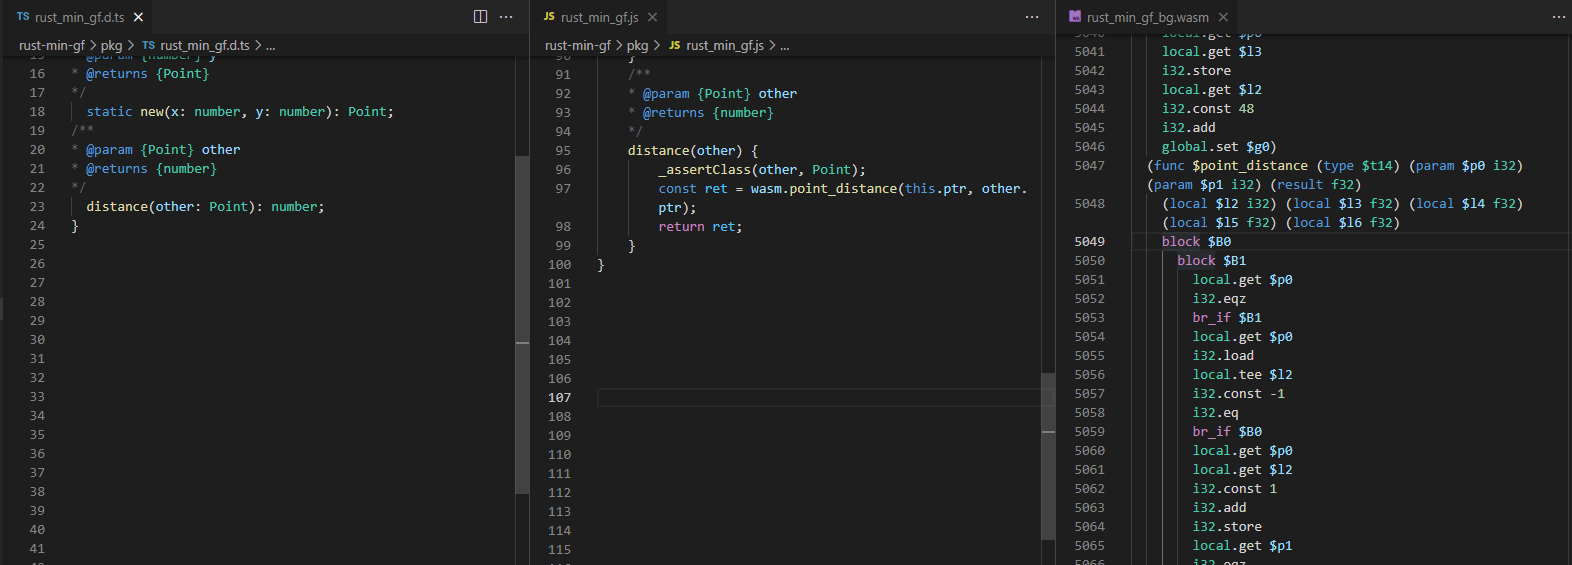
\includegraphics[width=\linewidth]{13.PNG}
  \caption[compilation artifacts]{wasm-pack Compilation artifacts: A Typescript Declaration file, a javascript file, and a WebAssembly binary, visualized as WebAssembly Text (WAT). }
  \label{fig:rust-plugin:compilation-results}
\end{figure}

To load this project into Geofront, a reference to the path of the compilation artifacts must be specified within the Geofront GUI, shown in \reffig{fig:min-rust-plugin-import}.
A local path was used for convenience, instead of publishing this demo to npm, and accessing it via a \ac{CDN}.

\begin{figure}
  \graphicspath{{../../assets/images/6.1.1/}}
  \centering
  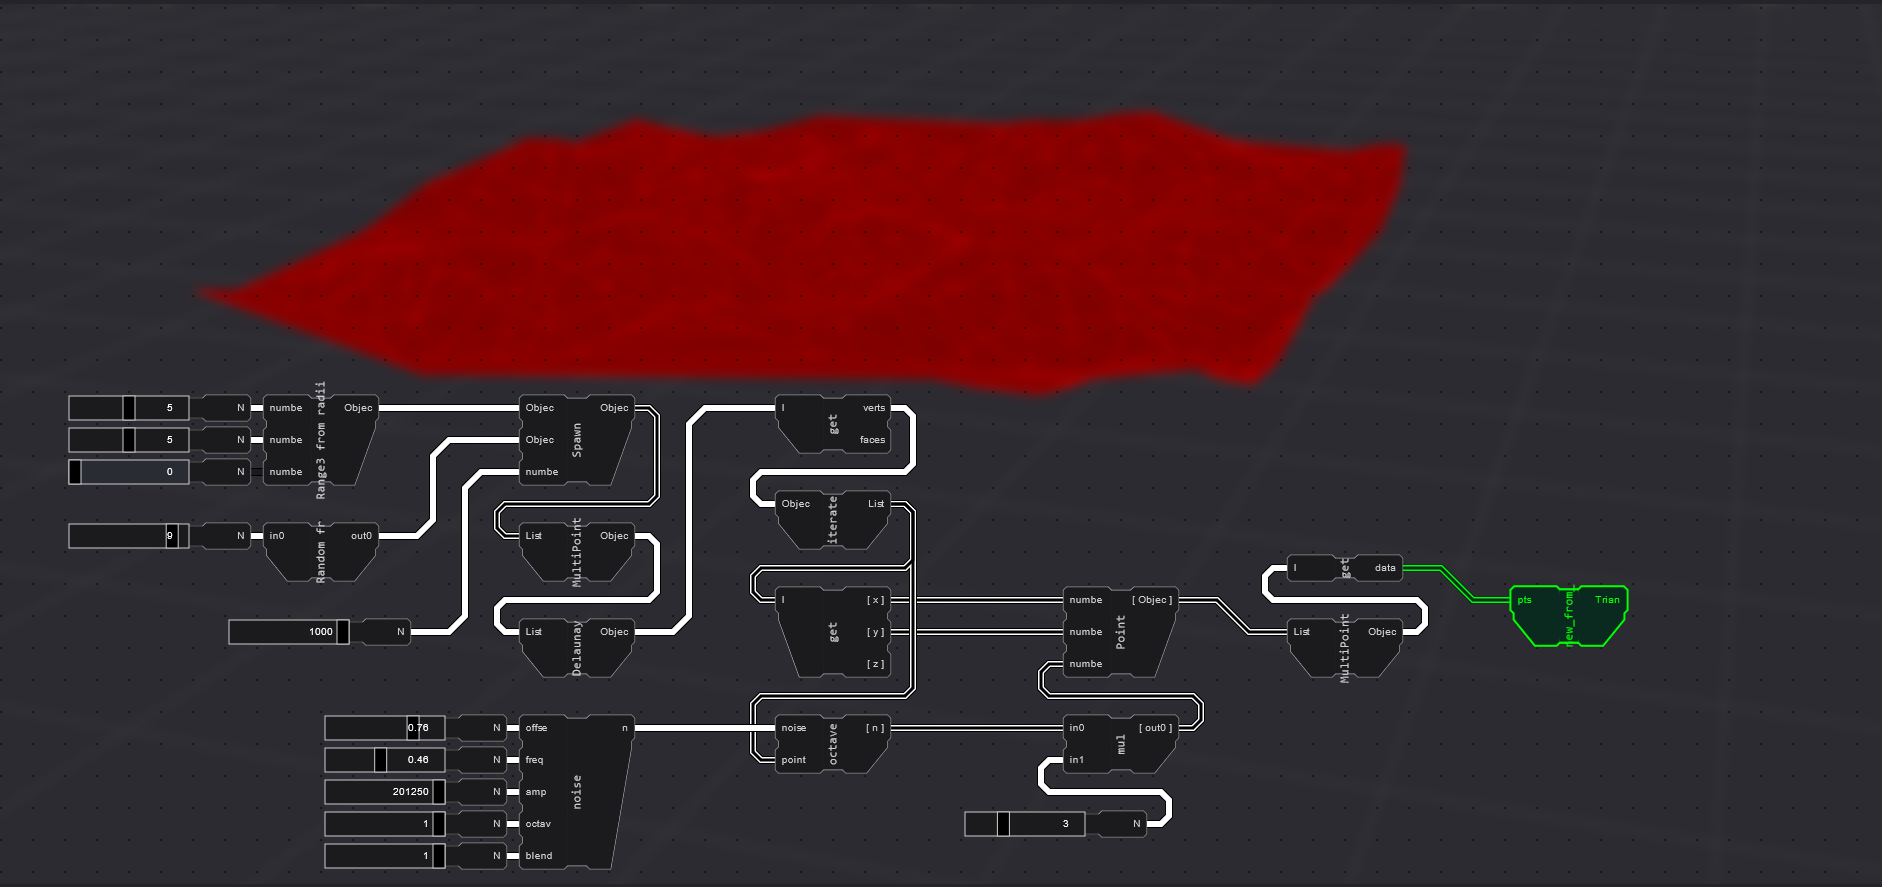
\includegraphics[width=0.50\linewidth]{2.PNG}
  \caption[loading a plugin]{Loading a plugin into Geofront using the \ac{GUI}}
  \label{fig:min-rust-plugin-import}
\end{figure}

\reffig{fig:rust-plugin-on-canvas:1} shows how all functions in this demo are loaded correctly, and \reffig{fig:rust-plugin-on-canvas:2} shows that the functions indeed work as expected to create two Graphs. 
Note how the parameter names and Types are also loaded, indicated by the names visualized at the input and output of the nodes.
This is thanks to the 'd.ts' file of \reffig{fig:rust-plugin:compilation-results}.

All in all, no problems were encountered.

\begin{figure}
  \centering
  \begin{subfigure}[b]{0.45\linewidth}
    \graphicspath{{../../assets/images/6.1.1/}}
    \centering
    \includegraphics[width=\linewidth]{7.PNG}
    \caption{}\label{fig:rust-plugin-on-canvas:1}
  \end{subfigure}%
  \qquad %-- that adds some space between th 2 figures
  \begin{subfigure}[b]{0.45\linewidth}
    \graphicspath{{../../assets/images/6.1.1/}}
    \centering
    \includegraphics[width=\linewidth]{6.PNG}
    \caption{}\label{fig:rust-plugin-on-canvas:2}
  \end{subfigure}%
  \caption[minimal rust geofront plugin: usage]{Usage On the canvas}
  \label{fig:rust-plugin-on-canvas}
\end{figure}

\subsection{Rust: Startin plugin}

Compilation of the \m{Startin} library was also successful. 
Startin already offered a wasm-ready library, this could directly be loaded into Geofront. 
However, the API exposed by this library used a non-functional style, making it hard to properly use the library on a VPL canvas. 
This is why a custom plugin library still had to be created, in which functions like '\m{new\_from\_vec}' were added to support functional usage. 

Other than that, all steps performed by the minimal Rust plugin could be made with this project as well, as shown in \reffig{fig:startin-plugin}. 
This also showcases the usage of the 'Renderable' bindings. 
This way, a variable of type 'Triangulation' can be viewed in 3D by clicking on it.

\begin{figure}
  \centering
  \begin{subfigure}[b]{0.90\linewidth}
    \graphicspath{{../../assets/images/6.1.2}}
    \centering
    \includegraphics[width=\linewidth]{1.PNG}
  \end{subfigure}%
  \\ 
  \begin{subfigure}[b]{0.90\linewidth}
    \graphicspath{{../../assets/images/6.1.2}}
    \centering
    \includegraphics[width=\linewidth]{5.PNG}
  \end{subfigure}%
  \\
  \begin{subfigure}[b]{0.90\linewidth}
    \graphicspath{{../../assets/images/6.1.2}}
    \centering
    \includegraphics[width=\linewidth]{2.PNG}
  \end{subfigure}%
  \caption[Types of \ac{vpl}s]{Startin, loaded as plugin within Geofront}%
  \label{fig:startin-plugin}
  \end{figure}

\subsection{C++: Minimal plugin}  

\begin{note}
  TODO: make this better
  HUGO: please explain interfacing troubles better
\end{note}

Making a minimal C++ plugin work in a Geofront graph was unsuccessful.
It was, however, possible to compile the plugin file to WebAssembly, and to use it in a web demo, but this was not without limitations. 

First of all, the construction of the C++ source code itself.
Emscripten's \m{embind} tool uses a macro syntax to flag functions marked for javascript compilation, shown in \reffig{fig:min-cpp-source}. 

While it does work similar to Rusts \m{wasm-bindgen}, cpp macro's do not allow for any pre-compile-time code checking, and can produce hard to decipher error messages. 

Secondly, to compile this file to the right binary with accompanied javascript wrapper, it had to be compiled using the relatively unknown \m{-sMODULARIZE=1} and \m{-sEXPORT\_ES6=1} flags enabled.
Otherwise, the javascript produced uses an import syntax too deviant from regular import statements to have any chance to be loaded into Geofront. 
It must be noted that emscripten was behind on documentation compared to 'wasm-pack' and the rust-wasm organization \citep{contributors_wasm-pack_2022}. 
it does not offer many examples, or thorough explanations on what many of the compiler flags do or mean \citep{emscripten_organization_emscripten_2022}.
wasm-pack on the other hand offers complete tutorials, a range of starter projects, and elaborate documentation of most of its functionalities. 

Thirdly, the compilation with the right flags enabled resulted in a valid '\m{wasm}' and '\m{js}' file, but not a '\m{d.ts}' file.
Emscripten does not support typescript declaration files, and third-party tooling to add this is only conceptual at this point in time. 
So, while this does allow for a working web demo similar to the Rust equivalent, shown in \reffig{fig:min-cpp-demo}, this makes it hard to determine the content of both files programmatically. 
This was partially solved by using javascript reflection.
By creating a blacklist of all 134 default functions the emscripten javascript wrapper comes with with the aforementioned flags enabled, we can distill the imported module down to the 2 symbols exposed by embind in this case, the \m{add} function and \m{Point} class.
However, by doing this, all function types and the names of all parameters are lost, and can not be loaded into Geofront, which in turn does not allow the resulting Geofront graph to be type safe. 
Another solution would have been to add static information about the functions and function types as strings in the CPP file, but this would have been a too manual of a solution to a problem which should be able to be solved automatically, as 'wasm-pack' did.

Finally, with a custom system in place to load embind files, the plugin loader could attempt to load both the js and wasm file. 
It is here were an obstacle was encountered, which could not be solved within the time frame of this study. 
The JavaScript wrapper file dynamically fetches the WebAssembly file. 
This is allowed when importing a javascript library in a regular, modern fashion. 
However, this is incompatible with the implementation choices of the Geofront plugin loader. 
To load a plugin dynamically, it fetches and interprets the source files at runtime. 
However, for security reasons, dynamically fetching a wasm file within these runtime interpretations is not allowed.
The \m{wasm-pack} solution does not have the same problem, for it allows the WebAssembly file to be parsed within its initialization function.
A change within the emscripten javascript wrapper would allow this obstacle to be overcome, but this must be left to subsequent research. 

\begin{figure}
  \graphicspath{{../../assets/images/6.1.3}}
  \centering
  \includegraphics[width=0.50\linewidth]{demo.PNG}
  \caption[loading a plugin]{Cpp-wasm web demo}
  \label{fig:min-cpp-demo}
\end{figure}

\begin{figure}
  \graphicspath{{../../assets/images/6.1.3/}}
  \centering
  \includegraphics[width=0.50\linewidth]{source.PNG}
  \caption[loading a plugin]{Cpp Plugin Source file}
  \label{fig:min-cpp-source}
\end{figure}

\begin{figure}
  \graphicspath{{../../assets/images/6.1.3/}}
  \centering
  \includegraphics[width=0.50\linewidth]{blacklist.PNG}
  \caption[loading a plugin]{Emscripten JavaScript wrapper blacklist }
  \label{fig:min-cpp-whitelist}
\end{figure}

\subsection{C++: CGAL plugin}

If the minimum cpp plugin example could not be loaded into Geofront, it will be unsurprising that the entirety of CGAL could also not be compiled into a suitable format ready for VPL consumption.
Several steps towards this goal were made however.

A web demo was able to utilize the CGAL kernel \reffig{fig:cgal-tryout-2}, for basic operations. 
Additionally, A subsequent web demo can utilize the CGAL TIN to a limited extent \reffig{fig:cgal-tryout-3}.

However, this study too could not be fully completed within the time frame of this study. 
Two problems prevented completion:

The first one has to do with rewriting inputs and outputs to CGAL functionality.
The most common ways to provide CGAL functions with data, and to retrieve results, is to read and write files. 
While this can be used on the web, the virtual file system wrappers presented by Emscripten add irregular syntax to the plugin, again compromising any chance it can be loaded into Geofront.
So, a way is needed to present CGAL with data directly from javascript or other wasm binaries, without reading or writing files. 
Initial tests were performed by parsing input data as a string buffer, which could then be 'read' like a file by CGAL.

The second issue with this process is to make sure all dependencies, like Boost, are compiled together with CGAL.
Legacy makefile build systems complicate this process. 
To get the current demo's working, several dependencies and sub-dependencies had to be manually traversed, their makefiles had to be edited, and the projects had to be re-compiled and copied to different location, to be used by the emscripten compiler exclusively. 
This is an unsustainable workflow, which will complicate development.  

% Additionally, many scientifically oriented C++ libraries like CGAL make extensive use of meta programming and template programming, paradigms which do not translate well to an environment outside of C++. 

\begin{figure}
  \graphicspath{{../../assets/images/6.1.4/}}
  \centering
  \includegraphics[width=\linewidth]{demo-2.PNG}
  \caption[loading a plugin]{CGAL Kernel Demo}
  \label{fig:cgal-tryout-2}
\end{figure}

\begin{figure}
  \graphicspath{{../../assets/images/6.1.4/}}
  \centering
  \includegraphics[width=0.50\linewidth]{demo-3.PNG}
  \caption[loading a plugin]{CGAL Triangulation Demo}
  \label{fig:cgal-tryout-3}
\end{figure}

\newpage
\subsection{Comparison}

\subsubsection*{Size}

Combined size of all compiler artifacts produced by wasm-back / emscripten:

\begin{lstlisting}

  wasm-pack:
  rust min:       20140 bytes 
  startin:       114263 bytes 

  emscripten:
  cpp min:        68424 bytes (3.4 times more)
  cgal tin test  257994 bytes (2.3 times more)

\end{lstlisting}

It is safe to say that the emscripten wrappers are significantly heavier, especially given the fact that the wasm-pack artifacts include typescript header files and were not optimized for size, while the cpp builds where.

This study speculates this difference could be because emscripten's primary use-case is compiling complete applications. 
This requires a more heavy wrapper, offering features like file servers. 
When compiling sizable C++ applications, the overhead of this wrapper can be marginalized.
However, apparently, emscripten is not able to distinguish between full applications, and small, granular use-cases like this one, and must include the 'full emscripten runtime' in all cases.

\subsubsection*{Performance}

The performance benchmarks. 
These benchmarks primarily test how performant the \\ javascript - WebAssembly interactions are. 

\begin{lstlisting}

  100.000 iterations:

  init: 
  rust min:       59 ms +/-  8 * SD
  cpp  min:       71 ms +/-  6 * SD
  js   min:        0 ms

  process: 
  rust min:      131 ms +/-  5 * SD
  cpp  min:      967 ms +/- 30 * SD
  js   min:       22 ms +/-  2 * SD
\end{lstlisting}

The scripts run are shown in \reffig{fig:perf-benchmark}.

These results also clearly show the emscripten wrapper is not able to compete with the wasm-pack solution.
From experimentation, performance hit could be narrowed down to initialization step of the 'Point' classes. 

These results may suggest two phenomena:
One, just like the artifact size comparison, this difference could be because emscripten is written from the point of view of a C++ application, and use case does not require custom javascript - C++ interoperability. 
A full application compiled with emscripten only needs to address javascript through emscripten own interface, which could be more performant. 
A full application seldom needs access to specific javascript processes the way this demo does. 

And two, the C++ builds may be suffering from 'legacy burden', as described by \citet{ammann_maplibre-rs_2022}. 
The emscripten solution needs to take more edge cases into account, has more complicated dependencies, and software compiled using emscripten must be more heterogenous than a younger language like Rust.
This all could lead to a significant performance hit.

\begin{figure}
  \centering
  \begin{subfigure}[b]{0.32\linewidth}
    \graphicspath{{../../assets/images/6.1.5/}}
    \centering
    \includegraphics[width=\linewidth]{rust.PNG}
    \caption{}
  \end{subfigure}%
  \qquad %-- that adds some space between th 2 figures
  \begin{subfigure}[b]{0.32\linewidth}
    \graphicspath{{../../assets/images/6.1.5/}}
    \centering
    \includegraphics[width=\linewidth]{cpp.PNG}
    \caption{}
  \end{subfigure}%
  \qquad
  \begin{subfigure}[b]{0.32\linewidth}
    \graphicspath{{../../assets/images/6.1.5/}}
    \centering
    \includegraphics[width=\linewidth]{js.PNG}
    \caption{}
  \end{subfigure}%
  \caption[benchmark]{Rust vs C++ vs js performance benchmarks}
  \label{fig:perf-benchmark}
\end{figure}


\section{Demo applications}
\label{sec:testing:demo}
% - Show a demo
This section demonstrates the extend to which Geofront is able to perform the main role it set out to fulfill: 
Accessing functions from low level \ac{GIS} libraries from within a web VPL, and subjecting these functions to to interactive elements, so that these functions may be used in different ways by end users.

Two related demo applications are presented, both featuring the \m{startin} library covered in \refsec{sec:testing:compilation}.
The following two sections demonstrate the achieved functionality, and implications of said functionality. 
the last section presents the limitations encountered during the writing and usage of these demo's.

\subsection{Demo One: Perlin noise \& startin}

\graphicspath{{../../assets/images/6/demo/}}

\begin{figure}
  \centering
  \begin{subfigure}[b]{0.90\linewidth}
    \centering
    \includegraphics[width=\linewidth]{products-1.PNG}
    \caption{}\label{fig:in-between-products:a}
  \end{subfigure}%
  \\ 
  \begin{subfigure}[b]{0.90\linewidth}
    \centering
    \includegraphics[width=\linewidth]{products-2.PNG}
    \caption{}\label{fig:in-between-products:b}
  \end{subfigure}%
  \\
  \begin{subfigure}[b]{0.90\linewidth}
    \centering
    \includegraphics[width=\linewidth]{products-3.PNG}
    \caption{}\label{fig:in-between-products:c}
  \end{subfigure}%
  \caption[Types of \ac{vpl}s]{Visual inspection of in-between products}%
  \label{fig:in-between-products}
\end{figure}

\begin{figure}
  \centering
  \begin{subfigure}[b]{0.90\linewidth}
    \centering
    \includegraphics[width=\linewidth]{explore-1.PNG}
  \end{subfigure}%
  \\ 
  \begin{subfigure}[b]{0.90\linewidth}
    \centering
    \includegraphics[width=\linewidth]{explore-2.PNG}
  \end{subfigure}%
  \\
  \begin{subfigure}[b]{0.90\linewidth}
    \centering
    \includegraphics[width=\linewidth]{explore-3.PNG}
  \end{subfigure}%
  \caption[Types of \ac{vpl}s]{Exploration of the effects of different parameters}%
  \label{fig:parametrization}
\end{figure}


The first demo application demonstrate Geofronts core ability to connect a native library to an arbitrary UI. 
In this hypothetical scenario, we wish to discover how the \m{startin} triangulation reacts to various terrains by subjecting it to different point samples: Smooth samples, noisy samples, homogenous or heterogenous point distribution.

In reality, the \m{startin} triangulation serves as a normal 2.5D delaunay triangulation, so we do not expect to see any strange behavior, but one can imagine other terrain extraction and generalization algorithms where a test like this would grant valuable insights.  
An example of such an algorithm would be a plane fitting algorithm using RANSAC or least squares adjustment.

A test setup is made to generate various terrains using Perlin Noise (SOURCE: KEN PERLIN), so that different landscapes can be simulated.

The resulting geometry pipeline can be seen in \reffig{fig:in-between-products}. 
A UI is created by using multiple slider widget as inputs numbers.
These numbers are used to create a bounding box area, which is subsequently filled with a random distribution of points (\reffig{fig:in-between-products:a}).
The input sliders are also used to construct a noise field, which is sampled using these points. These noise values are used as the heights of the points (\reffig{fig:in-between-products:b}).
Lastly, these points are used as input for the \ac{TIN} (\reffig{fig:in-between-products:c}).

Multiple observations can be made from this demo:
Firstly, note how the various visualizations of in-between products could be inspected by selecting the corresponding operation (\reffig{fig:in-between-products}). 
Secondly, observe how by connecting \m{startin} to this arbitrary \ac{GUI}, the behavior of the library can now be explored with different parameters (\reffig{fig:parametrization}).
Thirdly, recall that this sequence can be altered in real time, without any software alterations. 
These functionalities in conjunction are all indicators that Geofront can indeed be used to inspect the capabilities and quality of native \ac{GIS} libraries.

\subsection{Demo One: DTM \& DSM extraction}

\begin{figure}
  \centering
  \begin{subfigure}[b]{0.90\linewidth}
    \centering
    \includegraphics[width=\linewidth]{potree-1.PNG}
  \end{subfigure}%
  \caption[]{DSM and DTM extraction using Potree within Geofront}%
  \label{fig:potree-overview}
\end{figure}

\begin{figure}
  \centering
  \begin{subfigure}[b]{0.90\linewidth}
    \centering
    \includegraphics[width=\linewidth]{potree-2.PNG}
    \caption{}\label{fig:potree:a}
  \end{subfigure}%
  \\
  \begin{subfigure}[b]{0.90\linewidth}
    \centering
    \includegraphics[width=\linewidth]{potree-4.PNG}
    \caption{}\label{fig:potree:b}
  \end{subfigure}%
  \\
  \begin{subfigure}[b]{0.90\linewidth}
    \centering
    \includegraphics[width=\linewidth]{potree-5.PNG}
    \caption{}\label{fig:potree:c}
  \end{subfigure}%
  \\
  \caption[]{Options when using Potree within Geofront}%
  \label{fig:potree}
\end{figure}

\begin{figure}
  \begin{subfigure}[b]{0.90\linewidth}
    \centering
    \includegraphics[width=\linewidth]{potree-7.PNG}
  \end{subfigure}%
  \caption{Resulting obj mesh, extracted from potree}
  \label{fig:potree-result}
\end{figure}

Geofront was meant not only to be used to examine and visualize native libraries, but also to directly utilize them to fulfill real applications.
This second application demonstrates the extend to which this is possible. 

The hypothetical scenario used for this demo, is a situation in which a small scale DTM is required from a point cloud. 
One could imagine a DSM or DTM of a construction site, required for creating an accurate render of a buildings surroundings. 

the above \m{startin} demo is used as a starting point. 
This time, however, the TIN will be generated from a real point cloud, instead of a simulated one, and will be converted to a \m{.obj} file, so that the DTM / DSM might be used in a different process. 

The resulting pipeline can be seen in \reffig{fig:potree-overview}. 
Central to this pipeline is the 'Potree applet', found at the start of the pipeline. This is a special type of \ac{UI} widget, which can be used to open a new browser window, running a second application, which was created using the Potree viewer (source: POTREE). 
This application can run independently, but by opening it from within Geofront, a connection between the two applications can be established. 
It allows Geofront to request a pointcloud, by pointing to a publicly hosted, potree-converted dataset. 
The same connection allows Geofront to request parts of this pointcloud, so that a sub section can be used in the Geofront pipeline. 
To query a specific subset, the Potree viewer itself can be used to:
\begin{itemize}
  \item Filter the density of the pointcloud to a desired LOD.
  \item Filter the pointcloud to a certain bounding box or polygon.
  \item Filter the pointcloud based on classifications, so that either 
  a DSM with all point (\reffig{fig:potree:a}),
  a DTM with only terrain (\reffig{fig:potree:b}), or
  a DSM with only buildings (\reffig{fig:potree:c}) can be created.
\end{itemize}

The pointcloud subset is then loaded into the Geofront pipeline, after it can be used as input for any loaded plugin. 
In this case, the points are inserted to the \m{startin} triangulator, after which the resulting mesh is converted to an \m{.obj} string, and made available for download using a 'save file' widget, so it could be used in a render (\reffig{fig:potree-result}).


Multiple observations can be made based on this demo.
First, notice again how all steps mentioned correspond to the nodes of the pipeline. 
None of these steps are final. 
A different application could be created at runtime, by for example, adding a \m{laz} writer component to save the resulting subset as a point cloud itself, or by using a component to perform a solar potential analysis. 
This application strongly suggests that Geofront can indeed be used to directly utilize native libraries as part of a "real" use-case.
Additionally, it demonstrates that Geofront allows not only composability between libraries, but also between libraries and full-scale, existing applications.

\subsection{Limitations}

Based on the above demo's, the following limitations in utilization were encountered: 
\begin{itemize}
  \item \textbf{Limited STD}: The standard operations and widgets present in geofront are limited. 
  examples of these are scaling a vector, filtering lists, or getting the highest point from a set.
  Additionally, standard \ac{GIS} functionalities, such as reprojections, are also not possible. 
  Currently, plugin libraries add some of these basic functions as a workaround.    

  \item \textbf{Types}: While the type system of Geofront is extensive and supports complex aspects such as generics, no clear design is present for interoperating between internal Geofront types, such as a Geofront Mesh, and a foreign type, such as \m{startin}s triangulation. 
  The method used in the above demo's involves breaking down a type into a basic javascript data formats, and using that as an interoperable model. 
  However, this relies on unsustainable parsers which use hardcoded strings, reflection, and "blind thrust".

  \item \textbf{Visualization}: Currently, the application is only able to visualize a small number of data types, like points, lines, and meshes. Geofront's source code will have to be altered to support a library using images, for example.
  Another visualization shortcoming is that meshes currently cannot support over 65.535 vertices. 
  
  \item \textbf{Performance}: The geofront runtime is not offloaded to a different thread, due to the difficulty of integrating web workers. 
  This means that heavy calculations performed on the canvas will freeze up the \ac{GUI} of the  application. 
  % which is not reasonable.  
 
\end{itemize} 

% - Show a bit of performance of said demo

\section{Comparison}
\label{sec:testing:features}

Geofront is 

TODO make a table, comparing features of geofront to grasshopper, geoflow, geometry nodes, and mobius modeller









\begin{tabular}{||p{2.8cm}|l|l|l|l|l||}
                  & \emph{Grasshopper} & \emph{Blender} & \emph{Mobius} & \emph{Geoflow}    & \emph{Geofront}   \\
Plugin support    & \textbf{Yes}  & No*    & No     & \textbf{Yes} & \textbf{Yes} \\
Plugin language   & C\#  & -    & -     & C++ & Rust/Js/Ts** \\
plugin types      & \textbf{Yes}  & No      & No     & Unknown    & \textbf{Yes} \\
Scalable          & No          & No      & No               & \textbf{Yes} & No         \\
Web based         & No          & No      & \textbf{Yes}     & No           & \textbf{Yes} \\
Base GIS Nodes    & No          & No      & \textbf{Yes}     & \textbf{Yes} & No \\
GUI nodes         & \textbf{Yes} & \textbf{Yes}      & No     & No          & \textbf{Yes} \\

\end{tabular}

\begin{itemize}[ ]
  \item * Not without altering the source code of blender itself.
  \item ** theoretically, any language can  be used. 
  Practically, only Rust, JavasScript and TypeScript result in valid plugins. 
\end{itemize}

\subsection{Plugin Creation}

Geofront:

\begin{lstlisting}
// lib.rs

#[wasm_bindgen]
fn add(a: i32, b: i32) -> i32 {
  a + b
}
\end{lstlisting}




Blender Geometry nodes: 



Geoflow:

\begin{lstlisting}
// ...

class AddNode : public Node
{
public:
  using Node::Node;

  void init()
  {
    add_input("in1", typeid(int));
    add_input("in2", typeid(int));
    add_output("result", typeid(int));
  }

  std::string info()
  {
    std::string s;
    if (output("result").has_data())
      s = std::to_string(output("result").get<int>());
    return s;
  }

  void process()
  {
    auto in1 = input("a").get<int>();
    auto in2 = input("b").get<int>();
    std::this_thread::sleep_for(std::chrono::microseconds(200));
    output("result").set(int(in1 + in2));
  }
};
\end{lstlisting}

Grasshopper: 

\begin{lstlisting}
namespace MyPlugin
{
    public class AdderNode : GH_Component
    {
        public ComponentNodeFromString()
          : base("Add Integers",
            "Add",
            "This component adds two integer values",
            "My Plugin",
            "My Plugin Category")
        {
        }

        protected override void RegisterInputParams(GH_Component.GH_InputParamManager pManager)
        {
            pManager.AddIntegerParameter("a", "value A", GH_ParamAccess.item);
            pManager.AddIntegerParameter("b", "value B", GH_ParamAccess.item);
        }

        protected override void RegisterOutputParams(GH_Component.GH_OutputParamManager pManager)
        {
            pManager.AddIntegerParameter("R", "result", GH_ParamAccess.item);
        }

        protected override void SolveInstance(IGH_DataAccess DA)
        {
            int a;
            int b;
            DA.GetData(0, ref a);
            DA.GetData(1, ref b);
            int c = a + b;
            DA.SetData(0, c);
        }

        public override Guid ComponentGuid
        {
            get { return new Guid("197d2ec4-c3b1-47ed-8355-6af3b7612f01"); }
        }
    }
}
\end{lstlisting}


\section{Utilization assessment}
\label{sec:testing:usability}


This section offers an analysis on the usability of Geofront, according to the framework described by \cite[]{green_usability_1996}.

\subsubsection*{Abstraction gradient: What are the minimum and maximum levels of abstraction? Can fragments be encapsulated?}

Geofront was meant to support encapsulation. 
The need for re-using parts of a script as components / functions was deemed more important than the benefits of having no abstraction hierarchy (what you see is what you get).
An early prototype of Geofront did allow for encapsulation, by taking a subset of a Geofront script, and compiling it to a javascript subset. This could then be loaded by the library loader. 
However, the addition of special types of nodes, and features like iteration, invalidated the \m{geofront -> js} translator.
The translation is still possible, just not implemented.  
As such, if a user desires re-usable components and a lower abstraction level, they will need to write a Geofront library.

% \textbf{Suggestion for improvement:} re-implemented the 'compile to js' procedure.s
% (image of abstracting away a javascript subset)

\subsubsection*{Closeness of mapping: What 'programming games' need to be learned?}

Mapping a problem to a geofront script is intuitive for the most part.
Think of the operations needed to solve a problem, 
find the right libraries and nodes representing these operations,
and connect these nodes according to type. 
However, this mapping of problem and solution is hindered by the fact that Geofront needed to support iteration, shown in \reffig{fig:programming-game}. 

Based on the studies and experiences with existing VPLs \refsec{sec:background-vpl}, these types of 'iteration games' are known to be a significant hinder to the closeness of mapping principle.

\begin{figure}
  \graphicspath{{../../assets/images/6.2/}}
  \centering
  \includegraphics[width=\linewidth]{programming-game.PNG}
  \caption[]{An example of a 'programming game' within Geofront. The 'loop' toggle  indicates if an component should operate on a full list, or operate on all individual items within the list. 
  This can be used to iterate over a 'list of objects' column-wise, or row-wise. This is considered a 'game', since this is not an obvious interaction, and must be learned before properly using Geofront. }
  \label{fig:programming-game}
\end{figure}
 

\subsubsection*{Consistency: When some of the language has been learnt, how much of the rest can be inferred?}

\cite[]{green_usability_1996} notes on the difficulty of defining 'consistency' in language design, and chose to define it as a form of 'guessability'.

Geofront has introduced certain symbolic distinctions between graphical entities to aid this predictability. 
The biggest is the distinction between \m{operation} and \m{widget} components: 
operations are pure functions with inputs and outputs. 
widgets represent some 'outside world' interaction, like an input value, a file, or a web service. 
This way, 'special behavior' is isolated to widgets, making the rest of the script more predictable. 

In practice, certain inconsistencies within Geofront arise due to the open nature of the plugin system. 
the consistency of geofront is mitigated by a library with a very different notion of naming, or if the library chooses unusual input or output patterns. 
For example, a euclidean, 3D coordinate can be specified as a \m{Vector3} object, a struct, an array of three numbers, or three different x, y, z input parameters.
Then again, it is unclear if inconsistencies between the api's of a language's libraries are to be contributed to the inconsistency of the language as a whole. 

% \textbf{Suggestion for improvement:} Stabilize the api of the Geofront Standard Library.

\subsubsection*{Diffuseness: How many symbols or graphic entities are required to express a meaning?}

Geofront periodically suffers from the same 'Diffuseness' problems \cite[]{green_usability_1996} adheres to vpls general. 
That is, sometimes a surprising number of 'graphical entities' / nodes are required to represent a simple statement.  
This is apparent when representing simple mathematical calculations. 

Additionally, the flowchart can only represent linear processes. Many geoprocessing algorithms are iterative and make use of conditionals. These cannot easily be expressed in a Dataflow VPL. As such, these processes must happen within the context of a function, within a 'node'.

A widget evaluating a line of javascript could help improve diffuseness. For now, if a user desires to use dense mathematical statements, or functions with many conditionals and complex iteration, a Geofront Plugin should be created.

% (image of complex / simple mathematical calcluation in javascript and in geofront)

% \textbf{Suggestion for improvement:} These situations could be prevented by allowing scriptable components. 

\subsubsection*{Error- proneness: Does the design of the notation induce 'careless mistakes'?}

There are some errors the user can make  in Geofront that will not be immediately obvious. 
The biggest one is that there are no systems in place preventing large calculations. 
These might freeze up the application. 

To prevent this, the geofront interpreter should have been implemented to run on a separate thread, using a web worker. 
Besides this, in general, many systems are in place preventing errors, such as the type-safety used throughout geofront.
Also, by disallowing cyclical graphs, users cannot create infinite loops accidentally.

\subsubsection*{Hard mental operations: Are there places where the user needs to resort to fingers or pencilled annotation to keep track of what's happening?}

Geofront is developed specifically to prevent "Hard mental operations".
Following the dataflow paradigm explained in \refsec{sec:background:dataflow}, geofront chose to disallows cyclical patterns. 
This greatly reduces the complexity of possible graph configurations, and also causes all in-between results to be immutable or 'final'.
By then allowing these results to be inspected, and allowing the graph to be easily reconfigured, Geofront allows a workflow rooted in experimentation and 'play'.
Users do not need to 'keep track' or 'guess' how things work.
Instead, they can simply experience the behavior, and adjust the behavior until satisfied. 



\subsubsection*{Hidden dependencies: Is every dependency overtly indicated in both directions? Is the indication perceptual or only symbolic?}

The dimension of 'hidden dependencies' is another way the dataflow-paradigm is advantageous. 
The pure functions of a diagram-based vpl like Geofront make the language in general consistent and predictable.
However, there are two exceptions to this rule:
First, the \m{widget} nodes are allowed to produce side-effects, such as opening a window, asking for an input, making a web request, etc. 
These are required to provide geofront with interactive inputs and outputs.
The distinction between \m{widgets} and \m{}

And second, the pureness of functions can only be maintained if all Geofront libraries also exclusively use pure functions. 
There is no fail-safe in place to prevent the usage of a library containing functions with many side-effects. 

\subsubsection*{Premature commitment: Do programmers have to make decisions before they have the information they need?}

In general, Geofront requires almost no premature commitment. 
Or, rather, the level of premature commitment is in line with textual programming languages, in the sense that a user is always somewhat committed to the structure they themselves build. 

One practical way in which Geofront exceeds in this dimension of premature commitment, is that the application does not require a restart upon loading a new library. 
Users can add or remove libraries "on the fly". 
This is unlike any vpl studied at \refsec{sec:related-geovpl} or \refsec{sec:related-webvpl}.

One particular type of commitment users must be aware off, however, is the commitment to using a \ac{VPL} like Geofront in general.
The current version of Geofront does not support compilation to JavaScript yet, which would mitigate this premature commitment. 
% Therefore, 


\subsubsection*{Progressive evaluation: Can a partially-complete program be executed to obtain feedback on 'How am I doing'?}

Yes. 
As explained at the answer for the dimension of 'Hard mental operations', this is a core aspect in how Geofront achieves its interactivity and debugability, together with its ability to inspect parameters. 

% (Image: Show example)

\subsubsection*{Role- expressiveness: Can the reader see how each component of a program relates to the whole?}

as the authors of \cite[]{green_usability_1996} write: "The dimension of role-expressiveness is intended to describe how easy it is to answer the question 'what is this bit for?'"

One of the ways Geofront addressed this is by making a distinction between nodes possessing pure operations, and nodes producing side effects, like widgets. 

% sizeable phenomenon

% grootste boosdoener: looping is now a simple boolean toggle within a component. 
% This makes it very non-explicit, 

% This leads to another problem: the problem of declarative iterations within a vpl. 

\subsubsection*{Secondary notation: Can programmers use layout, color, other cues to convey extra meaning, above and beyond the 'official' semantics of the language?}

No, Geofront does not offer annotations in its current state, besides the way the nodes are configured on the canvas.  
Geofront does provide visual indicators for types, and for if a cable / variable represents a single item, or a list of items.

This could be improved by providing a way to annotate: to create groups, to write comments, etc. 
Type colors, or some other way to distinguish data based on iconography, would also improve the secondary notation principle.
% \textbf{Suggestion for improvement:} 
% \textbf{Suggestion for improvement:} Type colors would also be nice.

\subsubsection*{Viscosity: How much effort is required to perform a single change?}

Despite these efforts, the 'mouse intensive' interface of vpls like Geofront continues to be a hinder for viscosity.
Certain situations require excessive mouse interaction, like substituting a function with another function, but keeping all inputs the same.
In text, this would be as simple as a non-symbolic renaming of the called function.
In geofront, this requires a lot of reconfiguration of cables. 

Viscosity could be improved by creating special actions in the editor to perform these types of manipulations.  
%  - select multiple inputs, select multiple outputs: connect by height.
% rename node

\subsubsection*{Visibility: Is every part of the code simultaneously visible (assuming a large enough display), or it it at least possible to juxtapose any two parts side-by-side at will? If the code is dispersed, is it at least possible to know in what order to read it?}

All parts of the code are simultaneously visible, and geofront does not offer any way of creating new popups or screens.

% ## Case Studies

% ### Vector
% _Vector data retrieval, transformation, visualization_

% ### Raster 
% _Raster data retrieval, transformation, visualization_

% ### 6. Experiments 
% _Performance benchmark between rust-wasm / cpp-wasm / cgal-cpp-wasm / js / cli usage_

% ## Final 
% _Answer research questions ????_


%%%%%%%%%%%%%%%%%%%%%%%%%%%%%%%%%%%%%%%%%%%%%%%%%%%%%%%%%%%%%%%
%%%%%%%%%%%%%%%%%%%%%%%%%%%%%%%%%%%%%%%%%%%%%%%%%%%%%%%%%%%%%%%
%%%%%%%%%%%%%%%%%%%%%%%%%%%%%%%%%%%%%%%%%%%%%%%%%%%%%%%%%%%%%%%
%%%%%%%%%%%%%%%%%%%%%%%%%%%%%%%%%%%%%%%%%%%%%%%%%%%%%%%%%%%%%%%

% OLD OLD OLD OLD OLD OLD OLD OLD OLD OLD OLD OLD OLD OLD OLD


% We group the requirements listed at \refsec{sec:method-one} in a group of base features,
% a group of dataflow features, and a group of geometry features.


% \section{Experiments}

% \subsection{ Web Mapping Service }
% -> could work, must be captured in component
% -> streaming question

% \subsection{ Open Street Map }
% -> could be hooked up to the geojson viewer



% \section{ Performance }
% \subsection{Vector 3D}

% ....

% \subsection{Raster}

% ....

% \subsection{Geo features}

% ....


%%%%%%%%%%%%%%%%%%%%%%%%%%%%%%%%%%%%%%%%%%%%%%%%%%%%%%%%%%%%%%%%%%%%%%%%%
% \section{Use Case: Educational Sandbox}
% \begin{lstlisting}
% WHAT: 
%  - show the behaviour of a simple ransac algorithm, fitting a plane through 
%    a point cloud
%  - show it beharivourly: show in-between steps
%  - make parameters ajustable (number of high scores, minimum high score, 
%    number of tries, etc.)
%  - add least squares adjustment, and compare.

% SIMILAR EXAMPLES: 
%  - the geometric predicates explanation 
%  (https://observablehq.com/@mourner/non-robust-arithmetic-as-art)
%  - 

% ASSESS ON: 
%  - educational value
%  - ease of usage (the promise of **Criterium A**)
 
% ASSESSMENT (hypothesis): 
%  + indeed very insightful for analying the behaviour 
%    and operation of certain 
%    algorithms & parameters. Not many applications can show 
%    this level of insight. 
%  + feature B can be used to strip the tool down 
%    to the bare minimum,   helping 
%    with not overwhelming the user with features

%  - This VPL is not easy to operate. 
%    It remains difficult to communicate what needs to 
%    be done, how things work. This is not an expert tool, 
%    but also not a beginners' tool.
%  - No built-in tutorialization
%  - hard to discover the code underneath, 
%    obfuscating the link between process and code.

% \end{lstlisting}

% %%%%%%%%%%%%%%%%%%%%%%%%%%%%%%%%%%%%%%%%%%%%%%%%%%%%%%%%%%%%%%%%%%%%%%%%%
% \section{Use Case: Web Demo Environment}
% \begin{lstlisting}
%     WHAT:
%      - Show the startin delaunay triangulator
%      - Accept user-submitted Laz files as input
%        - filter the ground
%      - Accept a randomly generated point cloud based on perlin noise.
%      - Visualize the generated mesh, and make it available for download

%     EXAMPLES: 
%      - hugo's demo
    
%      ASSESS ON:
%      - **Criterium B**: extendability: 
%        - how does foreign and native codebases interact? 
%      - clarity
%      - reproducibility
%      - performance
%      - scope (raster / vector / 2D / 3D)

%     JUDGEMENTS (hypothesis): 
%      + Clarity is fine
%      + Reproducability is 
%      + Performance is decent

%      ~ clarity is fine, vpl allows users to 'play around' and try
%        different configurations, even run their own data through the
%        demonstrated functions

%      - Application is less suited for 2D 
    
% \end{lstlisting}


% \section{Use Case: Geoprocessing Environment}%%%%%%%%%%% SECTION
% \begin{lstlisting}

%     WHAT:
%       - Query an area of a point cloud with a polygon
%       - turn that area of points into a triangulation
%       - turn triangulation into isocurves
%       - save this as a geojson
%       - turn this whole thing into a function, which takes a PC, 
%         polygon and isocurve range, and spits out the geojson
%       - share this using a link
%       - turn this into an app?
%       - turn this into a script?

%     EXAMPLES: 
%      - 

%      ASSESS ON:
%      - **Criterium C**: Publicability:
%        - the ability to operationalize the application 
%        - can it be used by end-users? clarity? too much clutter

%     JUDGEMENTS (hypothesis): 
%       ~ sharing by link is possible, but for end-user usage, 
%         its very cluttered 
%       ~ compiling to js only partially works
%       ~ compiling into an app is not possible, but 
%         since everything runs client-side, it could be implemented. 

% \end{lstlisting}

% repeat results and answers in shortened form
\chapter{Conclusion}
\label{chap:conclusion}

% In this study we described the design, creation and evaluation of GeoFront, a web-based point-cloud processing tool.
% Overall, the study has succeeded in what it set out to do: designing and implementing a geo-web-vpl. 
% Moreover, it has delivered a workflow which can be used to quickly configure existing, native geoprocessing libraries written in C++ or Rust to be consumed and used by said geo-web-vpl.  

% This study concludes that based on these measurements, browser-based geo-computation is fast enough that it can enable 
% many promising use-cases, such as on-demand geodata processing apps, educational demo apps, and code sharing. 
% However, extensive user-group testing is required before any definitive statements on accessibility and fitness for geo-computation can be made.  

This chapter contains the conclusion of the study. 
It starts out by answering the research questions posed in the introduction (\refsec{sec:conclusion}), followed up by a summary of the most significant contributions (\refsec{sec:contribution}) and the limitations of these contributions (\refsec{sec:limitations}).
It continues by addressing points of discussion about this study (\refsec{sec:discussion}), which is followed by a number of theorized implications of this study (\refsec{sec:future-work}), and lastly, a reflection on the value and quality of this study
(\refsec{sec:reflection}).

% \begin{note}
%   Important: 
%   - Show what I have learned
%   - Show maturity
%   - Recommendations 
%   - Show balance
%   - Show finality
% \end{note}

%%%%%%%%%%%%%%%%%%%%%%%%%%%%%%%%%%%%%%%%%%%%%%%%%%%%%%%%%%%%%%%%%%%%%%%%%%%%%%%
%%%%%%%%%%%%%%%%%%%%%%%%%%%%%%%%%%%%%%%%%%%%%%%%%%%%%%%%%%%%%%%%%%%%%%%%%%%%%%%
%%%%%%%%%%%%%%%%%%%%%%%%%%%%%%%%%%%%%%%%%%%%%%%%%%%%%%%%%%%%%%%%%%%%%%%%%%%%%%%

\section{Conclusion}
\label{sec:conclusion}

This section answers the research questions. 
It starts with answering the sub research questions, and concludes with the answer to the main research question.

\subsection*{Sub Questions}

\begin{itemize}[ ]
  \item 1. "\myNewSubRQOne"
\end{itemize}

It turned out that two layers of \ac{GUI} features had to be created:

\textbf{Framework application}: Firstly, a base application was required to host the visual programming language, which needed to provide support for multiple windows, dropdown menu's, side menu's etc.
For this, a custom framework using Web Components was created, due to the absence of a desktop application-like framework in the javascript ecosystem. 
However, this did not provide the same level of tooling as a library like IMGUI \citep{cornut_dear_2022} or egui \citep{ernerfeldt_egui_2022}.
Because of this, in this area, the web context lead to a sub-optimal experience.

\textbf{The VPL}: Secondly, UI elements were required to form the interactive elements of the visual program itself. 
This GUI was given shape using a custom implementation. 
DOM events were used as inputs, and the Canvas API provided a way to visualize the VPL.
The web context provided two advantages here.
Firstly, a javascript program can access a large amount of features by default, such as this canvas API, but also WebGL. 
These features do not need to be included within the source code of the application, leading to quick load times. 
Secondly, by using \m{iframe's} and window pop-ups, the web context could be utilized to integrate third party UIs in a simple manner, as demonstrated with the Potree demo in \refsec{sec:testing:demo}.
Summarized, for this second set of \ac{GUI} features, the web platform was advantageous.

% Overall, the browser appears to be capable of representing a dataflow-type vpl graph to an acceptable degree, 
% based on the implementation presented in \refsec{sec:implementation:app}.

% All three of these features proved to be vital, and were performant enough to support an application like this. 
% Only the 2D canvas Api can become slow when rendering a great number of components. 

% TypeScript (JavaScript) was used to represent the data structure and logic needed to make a VPL functional. 
% Javascript's flexibility proved to be useful to support features like dynamically loading and using libraries at runtime. 
% However, TypeScript's limited type support at runtime, the absence of explicit immutability, and the limited precision in general (no integer atomic, only \m{number}), all hindered the implementation of the VPL model proposed.   

% % While the language does offers powerful options for reflection, this cannot truly be used if javascript itself makes no meaningful distinction between number types (\m{int, float, double}), for example.

% \begin{note}
% IMPORTANT
% - first-> a desktop-looking application to house the VPL
% - second layer-> UI features within the VPL itself to provide appropriate IO

% Both layers are fully implemented, and the web posed no fatal barriers. 

% PLUS: webgl, canvas API, and DOM: offered the right tools to build custom UI elements, and 3D viewers, with the advantage of not having to include UI libraries, leading to smaller data sizes 

% PLUS: web is very good in 'joining UI's'. This could be used 

% MINUS: most web tooling is 'locked into' the idea of websites. This made them hard to use for the purposes of a dynamic,
% 'desktop-looking' application.
% - Lead to custom solutions, and time investments which could have been spend on more important things than the UI.

% MINUS: performance  
% \end{note}

\begin{itemize}[ ]
  \item 2. "\myNewSubRQTwo"
\end{itemize}

Based on the features presented at \refsec{sec:testing:demo} and \refsec{sec:testing:features}, it can be stated that
the implementation was able to address all three discrepancies to a certain extent:

\textbf{1. Library capabilities get lost when used in an application}:
Because of the plugin system of this methodology, all functions which are included in a wasm compilation can eventually be accessed by a user. 
Additionally, the plugin boilerplate comparison of \refsec{sec:testing:features} showed that the no-boilerplate setup makes it simpler to add a new library as a plugin. 
Both features combined may lead to less features ending up 'lost in translation'.

\textbf{2. Applications are not further composable}:
The implementation showed that a web-based VPL can make existing applications composable, evident from the demo application presented in \refsec{sec:testing:demo}.
In this example, the Potree application was composed within a pipeline to extract a DTM or DSM, while retaining full functionality as a standalone application.

\textbf{3. A library offers no visualization or GUI by itself, and must be turned into an application before it can be used}:
Because the method presented in this study succeeded in combining \ac{GUI} components with low-entry barrier plugins, and because it allows the usage of unaffiliated WebAssembly projects, Geofront pipelines may act as a "custom GUI for any library" to an extend. 
In that sense, end users will only have to wait for a WebAssembly build, instead of a full application, before they are able to access a libraries content.

\begin{itemize}[ ]
  \item 3. "\myNewSubRQThree"
\end{itemize}

% The current methods of \emph{compiling} existing C / C++ geocomputation libraries to the web turned out to be insufficient for the purposes of this study.  
% This is due to emscripten's focus on compiling full C / C++ applications instead of libraries.
% Despite this, the study wás able to demonstrate how a novel method can be used to  \emph{compile} and \emph{load} a Rust-library for usage in the VPL.
% While not many contemporary geocomputation libraries are written in Rust, the study offers this method to either offer emscripten contributors a blueprint of a desired workflow, or to offer geocomputation library contributors a powerful use-case for the Rust language. 

The differences between C++ and Rust compilation are caused by the \\ difference in their respective WebAssembly compilers:
C / C++ requires the usage of emscripten and embind. 
Rust requires the usage of wasm-pack, and wasm-bindgen.

In the experiments performed by this study, significant differences were encountered between these compilers in terms of file size, supported features, and the performance of the produced 'glue code'.
The results of \refsec{sec:testing:compilation} showed that the emscripten compiler produced a binary which requires more than three times the size of the same functionality compiled with wasm-pack.
Interfacing this binary with JavaScript was between six and seven times as slow compared to the rust equivalent.

Moreover, emscripten lacked the interface features which were required to the purpose of using WebAssembly as a generic binding. 
wasm-pack provides type declarations in the shape of a TypeScript file, or by embedding them in WebAssembly using the proposed interface types \citep{wagner_interface_2022}. 
On top of that, it offered a strong binding system, allowing complex types such as a vector of floats (\m{Vec<f32>}) to be easily translatable to a javascript equivalent (\m{Float32Array}).

Regrettably, none of the above features were present in emscripten. 
Custom interventions were necessary on both the C++ end, and the JavaScript end, to get to a similar level of functionality.
However, these interventions made it so both ends need to be developed in relation to each other, which invalidates the  WebAssembly binary as a \emph{generic} interface.

Because wam-pack produces WebAssembly binaries with generic, simple, typed interfaces, Rust libraries could be used within the methodology presented in this study.
However, because binaries produced by emscripten did not possess these traits, C++ libraries could not be used within the methodology, meaning the goal of making core C / C++ GIS libraries more directly accessible could not be met.

All in all, it must be concluded that Rust-based WebAssembly compilation is more performant, more lightweight, and more feature rich compared to C++-based compilation.

% Emscripten can be used to compile full-scale C++ applications, and offers an emulation of a POSIX environment.
% However, it lacks support for compiling libraries themselves, compared to other wasm-library compilers.
% libraries generated with emscripten's 'embind' tool use irregular syntax, which troubles its ability to be loaded programmatically.
% While web implementations do exist like 'GDAL-js', these solutions are required to work though Web Workers, and use the emscripten virtual file systems, which again compromises their usage for the purpose of a dataflow-type vpl requiring pure functions.
% Finally, the experiments recognized certain discrepancies between the novelty of the WebAssembly format, juxtaposed to 50-year-old legacy of the C++ language, leading to larger wasm binaries, and less performant bindings compared to Rust.


\begin{itemize}[ ]
  \item 4. "\myNewSubRQFour"
\end{itemize}

Three measures were conceptualized and successfully implemented. 
However, all measures do have certain shortcomings. 
It must also be noted that all these measures are only presented 'in principle'.
Future work is required to verify their impact.

\begin{enumerate}
  \item \textbf{Portability}: The application uses native geocomputation libraries compiled to WebAssembly, 
  which makes the libraries behave the same way in the frontend, and in a potential back-end. \\
  \textbf{Effectiveness}: The effect of this is limited by the fact that \ac{wasm} binaries must for the time being be wrapped using javascript, due to the current lack of interface types. 
  This means that currently, a backend would require a javascript runtime to use these libraries.

  \item \textbf{Zero-cost abstraction}: The application uses a unique plugin system, to offer direct usage of javascript-wrapped libraries, and eventually WebAssembly-compiled libraries.
  This means that there is no difference between calling an operation in Geofront, and calling the function in the javascript-wrapped library.
  This allows a Geofront pipeline to be compiled to javascript, completely eliminating any explicit dependency to the 
  Geofront platform, the VPL model, or the \ac{GUI}.
  This is why Geofront can claim to use 'zero cost abstraction'. \\
  \textbf{Effectiveness}: A Geofront-to-javascript compiler was implemented and functional, but requires further study. 
  For example, it does not compile complex \ac{GUI} Widgets, and does not support iteration.
  
  \item \textbf{Locality}: Geofront is designed as a Dataflow VPL, which shares characteristics with functional programming. This leads to source code which can be reasoned about in a local manner, instead of a global one. This allow for parallelization. \\
  \textbf{Effectiveness}: The implementation of Geofront as a dataflow VPL was successful. However, due to limitations of the javascript language, the functional programming properties of the DataFlow VPL could not be strictly enforced. 
  Plugins must be trusted not to alter input data, or call global, state-altering functions, as functions could not be declared as 'pure', and variables cannot be declared as 'immutable'.

\end{enumerate}

\begin{itemize}[ ]
  \item 5. "\myNewSubRQFive"
\end{itemize}

% \begin{note}
%   TODO rewrite, this is a copy-paste from the overall conclusion!!
% \end{note}

Based on Table \ref{table:features} presented in \refsec{sec:testing:features}, Geofront provides a unique set of features. 
Comparable visual languages do not possess this exact combination. 
It offers relatively extensive plugin support compared to other VPLs, it is web based, and offers a range of \ac{GUI} nodes. 
Moreover, it is unique in its ability to accept third party Plugins written in different types of languages, and in the fact that it allows custom types within those plugins. 

% can be used to connect wasm-compiled libraries with almost any UI, making it able for end-users to access these 

% \begin{itemize}[ ]
%   \item 1. "\mySubRQOne"
% \end{itemize}

% The full answer of this question is represented by \refsec{sec:method:base-vpl} and \refsec{sec:implementation:app}.

% \begin{itemize}[ ]
%   \item 2. "\mySubRQTwo"
% \end{itemize}

% % To what extent can geocomputation libraries written in system-level languages be compiled
% % for web consumption?

% \begin{itemize}[ ]
%   \item 3. "\mySubRQThree"
% \end{itemize}

% Based on the method described in \refsec{sec:method:plugin-system} and \refsec{sec:implementation:loading}, and the analysis of \refsec{sec:testing:compilation}, it can be concluded that it is possible and even sufficiently usable to load a web-library into a VPL without explicit configuration. 
% It also had the desired effect of breaking down the barrier between vpl libraries and regular text-based libraries: Using this method, only one type of library is needed to serve both. 
% Moreover, it led to a workflow in which rapid experimentation was possible, since this method allows users to develop a library locally, and then quickly experiment and test its usage online. 

% The drawback of allowing this seamless interoperability and rapid experimentation, is that many important properties like descriptions and library metadata do not need to be explicitly specified, and could not be automatically extracted. 
% These properties still had to be added to the libraries in the shape of methods with a recognizable naming convention.

% Additionally, the freedom of granted by not restricting input and output types can lead to a confusing user experience, since there is no way of restricting libraries to use particular type convention.
% Even worse, the libraries could use references pointing to the same object, eliminating the 'immutable, no side effects' nature of a dataflow-type VPL.

% \begin{itemize}[ ]
%   \item 4. "\mySubRQFour"
% \end{itemize}
% % To what extent can a 'geo-web-vpl' be \textbf{used} to create geodata pipelines?

% Based on the analysis of Geofront in \refsec{sec:testing:usability}, it can be concluded that a geo-web-VPL can be used for geocomputation to a sufficient extent.  
% The analysis shows that many of Geofront's best aspects for the purpose of geocomputation are a consequence of the design decision to use a diagram-based, dataflow-type VPL.
% Examples of these are how the Functional programming paradigm leads to pure functions and immutable variables, making the graph as a whole behave in a predicable manner, allowing for the inspection of in-between data at runtime. 
% However, the openness of the plugin system inhibits the consistency of these functional aspects.
% Imported libraries are not forced to exclusively use pure function. 
% As a consequence, libraries can create functions with many side effects, or they can use inconsistent input and output datatypes, ultimately leading to confusion for the end-user.

\subsection*{Main Question}

\begin{itemize}[ ]
    \item "\myNewMainRQ"
\end{itemize}

Based on the answers to all supporting questions, The answer is a careful \textbf{yes}.

% A web-based VPL is a feasible method for providing direct access to native \ac{GIS} libraries.
The method is indeed capable of bringing native GIS capabilities from certain libraries directly into contact with end users, from within an application, without installation or configuration, and in a further composable manner. 
Compared to browser-based web applications, this method is more composable thanks to the dataflow-VPL implementation, 
and compared to the studied native VPLs, these functionalities are more directly available because of the static, web based implementation.
The method is also unique compared to studied web-based geometry VPLs, because of the plugin system, the range of different \ac{GUI} nodes, the dataflow VPL properties, and the proposed zero-cost abstraction runtime. 
All of these features combined lead to a VPL which is able to directly connect \ac{GUI} components with native \ac{GIS} libraries, all while remaining scalable in principle.

On a practical level, more work remains to proof this feasibility.
The methodology developed by this study is only \emph{theoretically} accessible and composable, based on achieved features. 
User-testing is required to confirm if this method indeed improves workflows, and actually saves time and energy of developers and end users. 
Moreover, the prototypical software implementation used is limited and not production ready.
% The 'no-boilerplate' plugin system cannot be used with
C / C++ \ac{GIS} libraries cannot be used in the method presented, which may or may not be fixed when the emscripten compiler adopts the Interface Types proposal. 
Additionally, the zero-cost abstraction runtime is non-functional, and must be improved upon in future work.

Despite all of this, based on the presented work, it is safe to say that visual programing methods, distribution using WebAssembly, and Rust-based GIS, all remain promising, valuable directions of future \ac{GIS} research.

% How can a VPL be used to support and execute existing geo-computation libraries in a browser?
% So, Does Geofront succeed in "converting existing geocomputation libraries to a sharable VPL format?" 

% A VPL can support existing geocomputation libraries if and only if these libraries are able to be \emph{compiled}, \emph{loaded}, and \emph{utilized} in a dataflow VPL format.

% Using a new javascript implementation of an acyclic, graph-based VPL, the study was able to demonstrate how the web platform can be used to represent a dataflow-VPL capable of hosting these libraries.
% The dataflow-properties of a graph-based VPL like this also makes this libraries sufficiently \emph{usable}, albeit with some well-known caveats of dataflow-VPLS, like the representation of conditionals and iteration. 


% All in all, this means that either if the Rust ecosystem gains more mature geocomputation libraries, or if Emscripten's capabilities improve, then the code portability problem \& dataflow problem of existing web-based geocomputation VPLS can be overcome. 



% This present a certain wider dilemma between Rust and C / C++.
% C / C++ has a mature foundation of existing geocomputation libraries.  
% However, this same legacy inhibits its portability, which makes it harder to use these libraries in novel ways, such as in web browsers. 
% For this study, this meant that the original goal of making core GIS libraries more accessible could not be met. 
% Rust is for the forseeable future a better choice for writing easily consumable, portable libraries, but does not have a fully mature ecosystem of geocomputation libraries yet. 

% To offer a solution, the study suggests that either emscripten's embind tool must be expanded to the level of functionality of wasm-bindgen, or geocomputation libraries must be rewritten in Rust. 
% This second option seems counterproductive, but as boldly stated by \citet{ammann_maplibre-rs_2022}: "innovation often requires selectively ignoring prior work."


%%%%%%%%%%%%%%%%%%%%%%%%%%%%%%%%%%%%%%%%%%%%%%%%%%%%%%%%%%%%%%%%%%%%%%%%%%%%%%%
%%%%%%%%%%%%%%%%%%%%%%%%%%%%%%%%%%%%%%%%%%%%%%%%%%%%%%%%%%%%%%%%%%%%%%%%%%%%%%%
%%%%%%%%%%%%%%%%%%%%%%%%%%%%%%%%%%%%%%%%%%%%%%%%%%%%%%%%%%%%%%%%%%%%%%%%%%%%%%%
%%%%%%%%%%%%%%%%%%%%%%%%%%%%%%%%%%%%%%%%%%%%%%%%%%%%%%%%%%%%%%%%%%%%%%%%%%%%%%%
%%%%%%%%%%%%%%%%%%%%%%%%%%%%%%%%%%%%%%%%%%%%%%%%%%%%%%%%%%%%%%%%%%%%%%%%%%%%%%%
%%%%%%%%%%%%%%%%%%%%%%%%%%%%%%%%%%%%%%%%%%%%%%%%%%%%%%%%%%%%%%%%%%%%%%%%%%%%%%%
%%%%%%%%%%%%%%%%%%%%%%%%%%%%%%%%%%%%%%%%%%%%%%%%%%%%%%%%%%%%%%%%%%%%%%%%%%%%%%%
%%%%%%%%%%%%%%%%%%%%%%%%%%%%%%%%%%%%%%%%%%%%%%%%%%%%%%%%%%%%%%%%%%%%%%%%%%%%%%%
%%%%%%%%%%%%%%%%%%%%%%%%%%%%%%%%%%%%%%%%%%%%%%%%%%%%%%%%%%%%%%%%%%%%%%%%%%%%%%%



\section{Contributions}
\label{sec:contribution}

The study was able to deliver two major contributions:
\begin{itemize}[-]
  \item \textbf{A new implementation of a web-based geocomputation VPL}
    This study introduces a novel javascript implementation of a web-based dataflow-VPL capable of both geometry processing, as well as geocomputation.
    Compared to existing web-based alternatives, this VPL is closer in design and functionality to common geometry VPLs like grasshopper, as it adheres to being a graph-based dataflow VPL. 
% We introduce the \"Geofront\" application, which achieves this accessibility in two ways: 
% Firstly, geoprocessing libraries, written in either Rust or C++, are compiled to WebAssembly: binaries which can be run in any modern browser, client-side. This mitigates the need for any installation, and allows the software to be directly used as soon as a website is fully loaded. WebAssembly offers a performance comparable to native usage. Geofront accepts these binaries as plugins.

% Secondly, Geofront itself is set up as a web-based visual programming environment, complete with a 3D viewer and WMS, WFS \& WMTS support. Using these tools, users can interactively run these geoprocessing libraries with different datasets and parameters. Using visual programming, the user can chain and alter geoprocessing steps, visualize in-between products, and save \& load these workflows.

  \item \textbf{A novel workflow of publishing and using native libraries on the web}
    Secondly, a new workflow was developed to allow a geo-computation function or library to be used within a visual programming environment.
    Moreover, this can be done with a minimum of configuration steps: 
    Any Javascript, Typescript or Rust library which satisfies the conditions layed out in \refsec{sec:implementation:loading:limits}, automatically functions in Geofront.
    
    % CITYJSON VALIDATOR ARGUMENT: THE WEB CAN BE USED TO IMMEDIATELY MAKE SOME TOOL / SOME RESEARCH PROJECT OPERATIONAL 'IN THE REAL WORLD'. THIS WAY, DATA CAN BE GATHERED, USER FEEDBACK CAN BE GATHERED, AND THE TOOL CAN BE EVALUATED IN TERMS OF REPRODUCABILITY. FINALLY, IT OFFERS THE POSSIBILITY OF THE TOOL BEING ACTUALLY USED, IN PRACTICE. 
% z
\end{itemize}

These two contributions together lead to an environment suited for a number of use cases, including: 
\begin{itemize}
  \item Visual debugging: One can use this environment visualize the result of an algorithm in 2D or 3D.
  \item Fine tuning parameters: In situations where algorithms contain unintuitive or empirically derived parameters (e.g. RANSAC), a visual environment can be use to quickly try out multiple settings, and to observe their effects.
  \item Benchmarking: Geofront can be used to test the web performance of multiple algorithms written in different languages. 
  \item Publication: Geofront scripts can be shared using a link. 
    this can be used to make a native library usable online, and by doing so, it may help to lower the delta between 'my library works for me' and 'my library works for someone else'.
\end{itemize} 
The combination of these features together make Geofront unique among both \\ geo-VPLS and web-VPLS. 
by providing the full source code, together will all implementation details given in \refchap{chap:implementation}, this study aims to provide guidance for all subsequent studies on the topic of VPLs, geocomputation, or geoweb applications using WebAssembly.



\section{Limitations}
\label{sec:limitations}

These contributions are bound by following limitations:
\begin{itemize}[-]
  \item \textbf{Only Rust, Js \& Ts library support}
  For now, only libraries written in Rust or Javascript / Typescript can be used in Geofront. 
  Due to the results layed out in \refsec{sec:testing:compilation}, a stable method of using any C++ library can not be provided for at the current moment.

  \item \textbf{In practice, not all libraries can be used }
  \refsec{sec:implementation:loading:limits} shows that not all Rust and JS/TS libraries are supported. 
  Additionally, in order to properly communicate, visualize, and make data interoperable, special 'config' functions and methods are still required. 
  
  \item \textbf{Only small-scale geodata is possible}
  the Geofront environment uses browser-based calculations, which does not lend itself well to process datasets larger than a certain threshold. 
  This means it cannot be used properly for big data, or other expensive processes. 

  % was not part of this study
  % First of all, the purpose of this study was only to get geocomputation libraries to the web, and inside of a vpl format. 
  
  
  % But still, lets give the devil his due:
  % Even when processing "smaller" datasets of, lets say 4 GB, most of the 'flowchart niceties' of geofront will cease to be useful. 
  % Inspecting this data will take more time than its worth, and reconfiguring the flowchart will take a long time. 
  % This can be mitigated by using web workers, but it will still not be very ergonomic to work with. 
  
  % When datasets become larger thansmall datasets of , most of the 'flowchart niceties' of geofront will cease to be useful. 

  \item \textbf{Implementation shortcomings} 
  Geofront is a prototype, and has many usability shortcomings, explained in \refsec{sec:testing:usability}.
  In addition, many geocomputation-specific aspects are missing, such as a topographical base layer.  
\end{itemize}



\section{Discussion}
\label{sec:discussion}
This section covers questions on the decisions made during the study, and the answer this study is able to provide as a response.

\subsubsection*{Q: Geodata is almost always big data. Will this web environment be scalable to handle big datasets?}

% 3. web interface
% - Having no file system really hurts the usefulness of the vpl as a data processing application.
% -> file system API is coming to fix this
% -> This study recommends cloud-native as a solution to this problem, and has added 

% One of the problems to address when considering the ergonomics of geocomputation, is the fact that geodata is almost always big data. 
% A web application cannot be expected to process huge datasets. 
% So how does geofront address this fundamental aspect of geoprocessing? 

The sizeable nature of geodata is a component fundamental to geocomputation.
However, scaling the application up to handle big data deviated too much from the core goal of this thesis to solve the problem of library portability, and had to be left to future work. 

Still, to pose a solution, this study experimented with compiling a \\ full Geofront script to javascript.
This can be regarded as a 'release' build of the Geocomputation pipeline: 
It would have allowed native CLI-execution using Deno \citep{contributors_deno_2022}, without any dependency or reference to Geofront itself.
Only the libraries used within the pipeline would need to be referenced, and this could have been done using regular javascript import statements, and npm.

% While it seems convoluted to compile a native library to WebAssembly and then execute it natively again, it is actually a sound strategy for building scalable, containerized programs for the cloud. 
% The 'WASI' project is a good example of this (Source: https://hacks.mozilla.org/2019/03/standardizing-wasi-a-webassembly-system-interface/). 
However, this experiment turned out to be a full-sized study in itself, and so had to be left to subsequent studies due to time constraints. 

\subsubsection*{Q: Why wasn't Geofront developed as a native application, and published to the web as a whole?}

A native-first build of Geofront would indeed be more performant, especially if the application is fully hybridized:
If both a native and web build of an application are available, then Users can choose for themselves if they wish to sacrifice the performance and native experience for the accessibility of a web build. 
 
However, many features key to the solution and workflow specific to Geofront would be lost in such a setup.  
(Prospected) features like dynamically loading plugins, scriptable components, or the compilation to javascript would be lost, or would have to be regained by incorporating a browser engine \emph{within} this native application. 

However, a valid criticism can be made that this study could have opted for adding more native-first components, such as the maplibre renderer \citep{ammann_maplibre-rs_2022}

% \subsubsection*{Q: Where was this 'barrier' the methodology spoke of?}

% Recall that the methodology states how the barrier preventing geo-web-VPLS from adapting native libraries, 
% must be because of issues encountered during \textbf{compilation}, \textbf{Loading}, \textbf{Representation}, or \textbf{used}, or a combination of these factors. 

% After the conclusion of this study, three major issues can be identified, which indeed occupy spaces in between the above four factors. 

% \textbf{1. Compilation and Loading}

% Firstly, it turned out to be challenging to expose existing libraries in a way usable by a dataflow-vpl. 
% - "just compiling to wasm" was not enough.
% - Webassembly is a double edged sword. Interfacing with wasm binaries from javascript is slow: lots of duplication of data. 
% -> catch 22 beyween rust and C++


% \textbf{2. Disconnect between textual and visual programming}

% Secondly, to turn a 'normal' function into a component usable in a dataflow graph, additional metadata needs to be specified.
% This leads to specific config files and classes, which in turns creates a barrier between regular programming libraries, and vpl libraries. 
% \refsec{sec:implementation:loading} represents the attempted solution to this problem. 


% \textbf{3. Web interfacing}

% And lastly, having limited access to the file system really hurts the usefulness of the vpl as a data processing application.
% This aspect has not been properly addressed during this study.
% This study recommends the novel web services cloud-native as a solution to this problem, and has added 


% \subsubsection*{Q: Is a geo-web-vpl the same as a 3D vpl with existing geoprocessing functionalities attached? In other words, is geoprocessing nothing else than procedural modelling?}

% No, but it is a good start. 
% A geo-web-vpl is \emph{at the very least} a Geometry VPL. 
% Indeed, an actual geocomputation vpl might require more features, such as a global CRS, support of base-maps, more control on precision, etc. 
% These important aspects must be left for future work.

% \subsubsection*{Q: Usage: Who benefits from a web-geo-vpl, and how? }
% This study proposes 4 use-cases:
% \begin{enumerate}[-]
%   \item Educational Sandbox
%   \item Web Demo Environment
%   \item End-user geoprocessing environment 
%   \item Rapid prototyping environment
% \end{enumerate}

% WHY DOES SOMEONE WANT TO TAKE EXISTING LIBRARIES AND TURN THEM INTO A WEB-BASED VPL FORMAT? 
% - interactive, visual debugging 
%   - explaining the behavior of algorithms to yourself and others
%   - why web: collaborative debugging
% - reproducability of results
%   - lowering the delta between "it works for me" and "it works for someone else"
% - improving the 'online presence' of research.
%   - making research results 'usable' via a link
%   - interdisciplinary exchange of ideas


% SO: Geofront is intended as a Computational Geometry Sandbox environment.
% Meant for: 
%  - publication
%  - sharing ideas 
%  - trying things out
%  - debugging code
%  - learning

% NOT for making programming as a whole 'easier'

\subsubsection*{Q: A large reason for developing web-based VPLs is accessibility.  Is this environment accessible?}

This study can only answer this question to a limited degree. 
Based on the analysis given at \refsec{sec:testing:usability}, it is safe to say that based on its features, Geofront is about as accessible as comparable geo-vpls, like Geoflow or Grasshopper. 
However, this analysis is only based on the achieved functionality and features. 
Actual user-testing is required to assess The true accessibility of the tool.

\subsubsection*{Q: Is this environment a competitor to native methods of geocomputation?}

In theory, yes.
Using the workflow as described, native geocomputation libraries could be used on the web at near native performance, without requiring installation.
Additionally, the web offers enough functionality so that even sizable, local datasets could be processed this way.
In practice, the dilemma between Rust and C++ means that in the sort term, this environment will not be used for professional geocomputation.
Additionally, the tool is still in a prototypical state, and will need to be more stable and reliable before being used professionally. 

%%%%%%%%%%%%%%%%%%%%%%%%%%%%%%%%%%%%%%%%%%%%%%%%%%%%%%%%%%%%%%%%%%%%%%%%%%%%%%%
%%%%%%%%%%%%%%%%%%%%%%%%%%%%%%%%%%%%%%%%%%%%%%%%%%%%%%%%%%%%%%%%%%%%%%%%%%%%%%%
%%%%%%%%%%%%%%%%%%%%%%%%%%%%%%%%%%%%%%%%%%%%%%%%%%%%%%%%%%%%%%%%%%%%%%%%%%%%%%%

\section{Future work}
\label{sec:future-work}
The many fields this study draws from mean that a great variety of auxiliary aspects were discovered during the execution ot the study. 
Some of these aspects are listed here, and could lead to interesting topics for follow-up research. 

\subsection{Cloud-native deployment \& scalability}

\begin{figure}
  \centering
  \begin{subfigure}[b]{0.80\linewidth}
    \centering
    \graphicspath{{../../assets/images/1/}}
    \includegraphics[width=\linewidth]{expanded-proposal.png}
  \end{subfigure}%
  \caption{An expanded proposed methodology, to provide a backend, cloud-based execution}
  \label{fig:proposal-extended-again}
\end{figure}

\begin{figure}
  \centering
  \graphicspath{ {../../assets/images/implementation/} }
  \includegraphics[width=\linewidth]{early-geofront.png}
  \caption[Geofront to js]{An early build of geofront, showing compilation to javascript}
  \label{fig:early-geofront-compile-to-js}
\end{figure}

An early build of Geofront had the ability to compile a Geofront script to regular javascript (see (\reffig{fig:early-geofront-compile-to-js})).  
All libraries were converted to normal import statement, all nodes were replaced by function calls, and the cables substituted by a variable token. 
This way, the application could be run headless (without the \ac{GUI}) either the browser or on a server, using a local javascript runtime like Deno \citep{contributors_deno_2022}.

A future study could re-implement this feature, opening up the possibility for deployment and scalability: 
Scripts created with geofront could then deployed as a web worker, as a web applications of themselves, or as a web processing services \citep{open_geospatial_consortium_web_2015}.
Also, by running this script on a server, and ideally a server containing the geodata required in the process, one could deploy and run a Geofront scripts on a massive scale. 

The overall purpose of this would be to create a \ac{FOSS} alternative to tools like the Google Earth Engine, and FME cloud compute. 

\subsection{Streamed, on demand geocomputation}

This study showed that browser-based geocomputation is reasonably viable. 
This might allow for a new type of geoprocessing workflow, which could replace some use-cases that now require big-data processing and storage.
A big problem in the \ac{GIS} industry is having to process and store sizable datasets, while only a portion of it will be actually used. 
A possible solution could be to take a raw dataset base layer, and process it on-demand in a browser.

This would have several advantages. 
First, end-users can specify the scope and parameters of this process, making the data immediately fine-tuned to the specific needs of this user. 
Secondly, this could be a more cost-effective method, as cloud computation \& Terabytes of storage are time consuming and expensive phenomena.

This type of \emph{on demand geocomputation} is certainly not a drop-in replacement for all use cases. 
But, in situations which can guarantee a 'local correctness', and if the scope asked by the used is not too large, this should be possible. 
Examples of this would be a streamed delaunay triangulation, TIN interpolation or color-band arithmetic. 

\subsection{Rust-based geocomputation \& cloud native geospatial}

An interesting aspect this study was able to touch on is using Rust for geocomputation.
The reason for this was the extensive support for webassembly, which was essential for browser-based geocomputation. 
However, there are additional reasons one might want to perform geocomputation within Rust.
One is that rust is widely considered as a more stable, less runtime error-prone language than C++, while offering similar performance and features.
Additionally, rust Wasm binaries also tend to be smaller than C++ wasm binaries.  

This could be very interesting to the "cloud-native geospatial" movement. 
This \ac{GIS} movement aims to create the tools necessary to send geocomputation to servers, rather than sending geodata to the places where they are processed.
To do this, geocomputation must become more portable than it currently is, and Rust compiled to WebAssembly might proof to be a strong candidate for creating exchangeable, performant, compact, and error-proof binaries.
It already sees usage on both cloud and edge servers (State of WebAssembly, 2022).  

Therefore, studying Rust-based geocomputation for the purpose of cloud native and edge computing, would be a promising topic for subsequent research. 

\subsection{FAIR geocomputation}

% The study has only scratched the surface on what is possible with combining geocomputation with the fields of Visual programming, and web applications. 
The introduction theorized on how both VPLS and web-apps could be used to make geocomputation less cumbersome.
The study chose to pursuit this on a practical, technical level. 

However, a more theoretical study could also be performed. 
It turns out that these ideas of 'less cumbersome geodata processing', have something in common with many of the geoweb studies on data accessibility and usability \citep{brink_geospatial_2018}.
The ideas of 'data silo's', 'FAIR geodata', and 'denichifying of \ac{GIS} data' (see \citet{brink_geospatial_2018}) map well to geocomputation:
Functionality Silo's, FAIR geocomputation, denichifying of \ac{GIS} computation. 

Therefore, an interesting question for a subsequent study could be: "How could geocomputation become more Findable, Accessible, Interoperable, and Reusable?", or "How to integrate the function-silo's of GIS, BIM \& CAD?"
By focussing on data processing actions rather than the data itself, we could shed a new light on why data discrepancies and inaccessibility exist. 
After all, if a user is unable to convert retrieved geodata to their particular use case, then the information they seek remains inaccessible.


% \subsection*{Reproducibility}
% This section provides a discussion on the reproducibility of the developed methods and obtained results in this study.


% \subsection{Hybrid geocomputation}

% Lastly, 


  
  % Sub component: FAIR: 
  % - FINDABLE:      Hard to find the right tools for the job
  % - ACCESSIBLE:    Hard to access these tools (install, setup environment, look at what you are doing)
  % - INTEROPERABLE: Hard to use two tools from different ecosystems (bindings, plugins, etc). 
  % - REUSABLE:      Hard to re-use a specific scripts written for one use case in another use case

% (NOTE: This is a nice point to make after the thesis: focus more on FAIR geoprocessing)

% The Geoweb, or Geospatial Web, covers a broad collection of topics located at intersection of the field of geo-information and the web. A noteworthy study on the Geoweb is Van den Brink's phd titled "Geospatial Data on the Web". \cite{brink_geospatial_2018}. She claims that even though geodata is vital to a diverse range of applications and people, the ability to properly retrieve geodata remains almost exclusive to experts in the field. This is to the determent of all these applications and people, jeopardizing value, opportunity, and decision making. She makes this argument by using the concept of FAIR geodata. Coined by \cite{mark_d_wilkinson_fair_2016}, The FAIR principles are a collection of four assessment criteria used to judge the usability of (scientific) data: Findable, Accessible, Interoperable, and Reusable. 

% We argue that if these concerns count for geodata \textit{retrieval}, they should just as well count for geodata \textit{processing}. After all, if a user is unable to convert the retrieved geodata to their particular use case, then the information they seek remains inaccessible. Therefore, this study introduces the concept of \emph{FAIR geoprocessing}. 

% Based on the arguments presented by \cite{brink_geospatial_2018}, we can also extrapolate that a \ac{gis} environment shouldn't exclusively be used by only experts. Van den Brink mentions a group called 'data users', presented as "web developers, data journalists etc. who use different kinds of data, including geospatial data, directly to create applications or visualizations that supply information to end users (citizens)". 

% We use both extrapolations to define the users and 'usability' for the context of this study. We will judge the proposed use case application as 'usable', if it is deemed Findable, Accessible, Interoperable, and Reusable. The user group intended to use this environment is defined as both experts in the field of geo-information and this more general group of data users.

% Function Silo's \& denichification of GIS

% similarly: function silo's 

% / experiment to assess: 
% - The fitness of the web in general for client-side geo-computation
% - If new features of modern browsers mean anything for the field of geo-informatics at large 
% - The topic of accessible geoprocessing.

% now, answer this to the best of your ability

% Many considerations

% Premature optimization is the root of all evil | Donald Knuth
% Delay decisions to the latest moments, to gain maximum context,
% Key insight into writing better compilers

% While conducting this research, I came across various key insights from various studies, and there seemed to be a link between them 

% Most important effort I saw is the "denichification" of the geospatial world.
% - Hugo's keynote
% - Linda van den Brink's PHD
% - cloud-native geospatial 

% We focus on Access

% \m{->} the fact of being able to be reached or obtained easily:
% \textit{Two new roads are being built to increase accessibility to the town centre.}

% \m{->} the quality of being easy to understand: 
% \textit{The accessibility of her plays means that she is able to reach a wide audience.}


%%%%%%%%%%%%%%%%%%%%%%%%%%%%%%%%%%%%%%%%%%%%%%%%%%%%%%%%%%%%%%%%%%%%%%%%%%%%%%%
%%%%%%%%%%%%%%%%%%%%%%%%%%%%%%%%%%%%%%%%%%%%%%%%%%%%%%%%%%%%%%%%%%%%%%%%%%%%%%%
%%%%%%%%%%%%%%%%%%%%%%%%%%%%%%%%%%%%%%%%%%%%%%%%%%%%%%%%%%%%%%%%%%%%%%%%%%%%%%%


% \subsection{Cloud Native}
% Lastly, the 

% - The front-end browser technologies are a vital component of the modern geospatial software.
% - Like how the entire cloud-native moment is only possible because of the HTTP range request feature. 

% - a vital component of the cloud-native geospatial moment is the "HTTP range request" web feature, and chris said as much.
%   - this feature has been out for some time ( html1/1, )
% - What I'm saying, is that we have a whole range of similar, 'game changing technologies' recently added to web browsers, and I have a feeling these features could be the birthing grounds for new, ground breaking ideas and movements of ideas. 

% We have not fully envisioned these new trends, nor do we have a catchy, powerful name such as \emph{Cloud Native Geospatial}, But I have no doubt that something revolutionary will come of this. 

% Nevertheless, I will attempt to name and envision a trend from these technologies. \emph{"FAIR Geodata Processing"}.

% Vision: 
% - Portable, cross-platform, binary geoprocessing libraries, which can be used on the cloud / on servers, natively, and in the browser, without any changes. 
% \m{->} we can use that to build standards for geodata processing itself. Every \m{GP} library interoperable with every other library, at least on a language and package manager level.
% - This also eliminates the need of platform specific plugins (QGIS plugins, ARCGIS plugins, Blender Plugins, 'web plugins').
% - This could lead to a generalized geoprocessing library portal like NPM / cargo / WAPM with an attached content delivery network, Or these infrastructures can just be utilized, with just an UI sprayed on top.

% - I am aware that these types of efforts have been attempted many times before, but WebAssembly might be a missing link 

% \m{->} webassembly has a good balance between portability and performance.

% \m{->}

% If I were to attempt to name this trend, I would


% \begin{note}
  
% recommendations: 
% - go native, since it is better suited for these types of applications
%   - native VPL 
%   - use a native GUI library
% \end{note}

\section{Reflection}
\label{sec:reflection}

Here I reflect on possible shortcomings of the thesis in terms of value and quality, and how I have attempted to address these shortcomings. 

\textbf{Biases regarding C++ and Rust}

First of all, in the comparison between C++ and Rust, the studies conducted proved to be unfavorable towards C++. 
it could be that C++ was judged unfairly, due to the authors personal inexperience with the build tooling of the language. 
Many complications were encountered during compilation, leading to extensive editing of makefiles and attempts at recompiling forked subdependencies of CGAL using 'hacky fixes'.  
It is unknown how much of this was due to personal C++ inexperience, inflexibility of the libraries in question, or the shortcomings of the toolchain. 

Despite this, the study performed steps to make the judgement as non-biased as possible.
Preliminary studies were conducted with both languages, and additional C++ courses were followed. 

It could even be the case that this particular study is more fair than a study conducted by authors with more experience with C++, 
since before the assessment between Rust and C++, approximately the same amount of time was spent with both languages. 

\textbf{Scope too wide}

Additionally, the scope generated by combining geocomputation, web applications and VPLs, might have been too extensive. 
This is evident in the number of 'supporting studies' conducted, and the sizable workload of the implementation.
A better approach might have been to focus the scope of the thesis down to only 'browser-based geocomputation', or 'visual programming and geo-computation', or 'geocomputation using rust', to allow for a more in-depth analysis.

On the other side, the core of the contribution of this thesis lies precisely in the attempt to connect these subjects,
especially since prior studies remained by en large closely scoped to their respective domains.
The hypothesis was that a certain synergy may exist, and that each separate domain stand to gain from the ideas and knowledge found in the other ones. 
In order to make this possible, the study had to acquire a scope to explore all in-between synergies and interactions, leading to geo-vpls, web-vpls, and browser-based geocomputation. 
Now that this study has made these connections explicit, future studies can focus on more precise aspects of these cornerstones again.

\textbf{Too distant from the field of GIS}

Where the exact boundary of one field of study is, and where another begins, remains of course a fuzzy question. 
Still, the direction of this study appears to stray far from 'core GIS concerns', and appears more in one line with the  field of "End User Development (EUD)", and fields like "Computer-Human interactions". 

In defense of this, the field of GIS, like all research, is built on top of more foundational work which came before it. 
However, during the implementation of the study, it appeared that little foundation was in place for a geo-web-vpl specifically. 
This made it necessary to generalize, to build the missing foundation first.
For example "How can \emph{any} library be compiled and loaded into \emph{any} web-vpl" is a question which had to be answered first. 
Then, the question could be specified to \emph{geometry} and \emph{geo-web-vpl}. 
And only after that, the geodata and geoprocessing libraries specific to the field of GIS could be regarded. 
By doing so, this study wishes to provide a foundation to assist any subsequent future study in this direction, which can then be more GIS focussed.

% \textbf{Imbalance between software implementation and study}

% The fourth 'danger' which remained an ongoing balancing act during the execution of this study, is the balance between 'performing a study' and 'developing an application'. 
% Indeed, many of the aspects discussed throughout this study come down to implementation aspects of the geofront application. 

% PROBLEM: WHAT DO I TEST??

% This is why the study has attempted to generalized its findings as much as possible.
% Geofront is regarded as a proxy of geo-web-VPLS in general, in the sense that whatever was encountered during implementation of the application, must be the same for any attempt at creating a web-based vpl for geocomputation.


\textbf{Subjectivity in qualitative assessment}

Lastly, many of the assessments made by this study are qualitative assessment, and as such, might suffer from a high level of subjectivity. 
This is unavoidable in any assessment which does not come down to clear, quantifiable aspects, such as performance, memory usage or precision. 

Nevertheless, the study has attempted to scope this subjectivity by basing its assessments heavily on prior works in the field of vpl, and always showcasing clear examples. 

% \section{Personal Reflection}
% \label{sec:personal-reflection}

% A thesis is, among many things, an attempt to formulate. 
% To clarify and structure a phenomenon, as much for yourself as for the public. 
% This thesis can also be regarded as such an attempt. 
% I tried to understand a phenomenon you might call: "End User Geodata Processing". 
% To what extent can the activity of geocomputation truly be made "publicly available", besides writing open source software?
% I see this in much similar terms to the "Teach a man how to fish..." saying.
% Providing open geodata to the public is great, but we might only be "Giving a man a fish so he can eat for a day".
% By providing geocomputation tools in a fashion usable by end users, we could give the general public more authorship and autonomy over geodata. 
% And, more concretely, if a person themselves can compute what they want, when they want it, we don't have to pre-process several variants of the same dataset, tweaked to suit different audiences, saving storage and especially processing time.

% I did not have this clear of a goal at the start of the thesis, only intuitions and a set of loosely coupled ideas.
% I was also unable to find a foundational body of work to base this research on. 
% What I did know is that I did not want to stay at a theoretical level. 
% I wanted to truly \textbf{build} a solution, to the at this point ill-defined problem. 

% In hindsight, I don't think it was wise to build a concrete software implementation based on multiple, loosely defined theories. 
% This imbalance led to a time-consuming complication between research and software implementation while writing the thesis.

% Nevertheless, through many iterations, I was eventually able to integrate both the ideas and the thesis at large with this software implementation.
% I have learned two additional major lessons from conducting this study: 
% One, writing well is hard work. 
% Boiling a story down to the essentials asks a great deal of time and energy. 
% I would not call the current story this study tells concise, but it is much more precise than I was able to write at the beginning of this adventure.

% And two, I must learn to rely on the work of others.
% This is difficult, as it is contrary to my personal conviction on the great importance of "learning from scratch".
% Both the software implementation and the written thesis had me figuring out a lot of aspects from scratch, and this had advantages and disadvantages.
% The advantage is that 'doing the work again yourself', is probably one of the most educational endeavors one can do. 
% We must understand the inner workings of the systems we work with, and especially of the systems we wish to improve. 
 
% This is why I took the risk of developing many aspects of this thesis anew. 
% Even if this might turn out to be a parallel study, it would only reinforce the 're' in research. 

% The disadvantage of doing this, is that you prevent yourself from being able to 'stand on the shoulders of giants'.
% I especially felt the sting of this lesson in the written aspect of this thesis. 
% Not really knowing up from down because of having no readily available work to build on caused countless hours of revision.
% Another great disadvantage is that you run the risk of alienating both yourself and your endeavors. 
% By building from existing starting points, you connect your work with the works of others, and in doing so contributing to a wider community.

% If you have read this thesis up to this point, I want to sincerely thank you for your time and interest.
% With this thesis, I hope to have provided you and the wider geospatial community with something of value.

% \section{Personal Reflection}

% One of the goals of this study was to investigate and explore browser-based geo-computation, and there are many ways of conducting exploitive studies. 
% This study chose for a practical approach: investigation by means of creating an application.
% The advantage of this approach is that it leads to tangible results. 

% The disadvantage of this approach is that software development can lead a study astray, if the development needs of the application are put before the needs of the study itself.

% This study was a battleground between "performing a study on if geocomputation benefits from the web \& a vpl", and "lets build an open-source tool to aid geocomputation"

% It needed a bit of both.


% \begin{note}
  
%   Reflection
  
%   "It is not the task of the University to offer what society asks for, but to give what society needs" ~ Edsger W. Dijkstra
  
%   Despite the cliche of quoting Dijkstra, and despite the arrogant danger of pretending to know what people want better than they themselves know what they want, 
  
  
%   'what the world wants is more react, angular, or vue developers'
%   'what the world needs, in my opinion, is guidance on this front of web vs native application development.'
  
%   right now, we are sucked in the rabbit hole of 'make everything web-based, then maybe try to execute that natively',
%   And I think that we should start working towards a situation of: 'make everything natively, KNOWING that publishing it on the web is a piece of cake'.
  
  
  
%   The thesis represents to me a bold "What if" scenario: 
%   - What if geodata computation was an elegant, ergonomic process?
%   - What if more people could more easily perform geospatial computations?
%   - What if textual and visual programming languages worked complimentary?    
%   - What if geocomputation libraries where written in Rust instead of C/C++?
%   - 
  
%   'we are not inventive enough with the tools at our disposal'
%   'outdated web vs native, client vs server distinctions block our vision from seeing new types of applications'
%   'we could be doing so much more with what we have.'
  
  
%   A huge leap 
  
  
% \end{note}
  
%   \subsection{Personal Motivation}
%   During my internship I was tasked with creating a parametric 3D CAD model. 
  
%   - local usage 
%     -> quick, direct feedback
  
%   - We needed to make this a product for end users. 
  
%   - Industry-standard choice: cloud 
%     -> smart-server dumb-client setup, cloud-native architecture 
  
%   - Problems
%     -> continuously downloading new resulting CAD files after every change created a lot of web traffic. 
%     -> slow, not at all the same experience.
%     -> cloud host was even more slow in cold-start scenario's   
%     -> cloud host monetization scheme: pay for every time the script runs, 
%        -> meant that consumers had to be discouraged to 'play around' with the tool too much. 
    
%   This made me question the cloud-based paradigm, at least for the use case of calculating geometry by end users. 
  
%   At the same time, many of our parametric designers could use grasshopper, and only grasshopper. 
  
%   This led me to think about a vpl which can run client-side in a browser, and can produce client-side applications.
  
%   if the data is geodata or CAD data, does not matter besides the fact that geodata is often big data.
  
  

%   \textbf{Motivation 2: Accessible Geoprocessing Libraries}
  
%   Most industry-standard geoprocessing libraries such as CGAL are difficult to use by anyone but experts in the field. A steep learning curve combined with relatively complex installation procedures hinders quick experimentation, demonstration, and widespread utilization of these powerful tools. It also limits the interdisciplinary exchange of knowledge, and compromises the return of investment the general public may expect of publicly funded research.
  
%   Geofront could improve the accessibility of existing geodata processing and analysis libraries, without adding major changes to those tools, by loading webassembly-compiled versions of them, similar to [other web demo's](todo).

% \subsection{Reproducibility}

% Results themselves are insanely reproducable.
% Software can be used, you can reproduce results easely by dumping versions of geofront in 
% a folder.

% \dots

% Software can also be build without too many difficulties, but the procedure has some unconventional build steps: 

% \dots

% BUT, the code is not the cleanest, nor the most conventional. minus points on open-source accessibility.

%%%%%%%%%%%%%%%%%%%%%%%%%%%%%%%%%%%%%%%%%%%%%%%%%%%%%%%%%%%%%%%%%%%%%%%%%%%%%%%
%%%%%%%%%%%%%%%%%%%%%%%%%%%%%%%%%%%%%%%%%%%%%%%%%%%%%%%%%%%%%%%%%%%%%%%%%%%%%%%
%%%%%%%%%%%%%%%%%%%%%%%%%%%%%%%%%%%%%%%%%%%%%%%%%%%%%%%%%%%%%%%%%%%%%%%%%%%%%%%

% \section{Self Assessment}

% \subsection{Using Geofront for CAD or BIM}

% \todo{make it more nuanced}
% % AT THE END OF THE DAY, THERE IS NO REAL DIFFERENCE BETWEEN CAD, BIM and GIS.
% % of course, there are many differences, like required precision and tolerances, which types of interfaces and operations are common, and the subject matter it represents. 
% % But on a deeper, fundamental level, they are all the same: its just a bunch of 2D / 3D data, representing some real world thing. 

% Today, we see the need for collaboration between CAD, BIM and GIS. Entire industries (Speckle, FME) have been introduced to bridge the gaps. 

% All three of CAD, BIM and GIS want the ability to join solids together, desire to give certain spatial objects metadata, and want to run automated workflows in the cloud. These Individual fields are constantly reinventing features the other fields have already figured out. BIM is starting to open up to the idea of streaming only a part of the building instead of the whole thing, something which the GIS world has been doing for years. On the other hand, GIS is only now starting to make the transition to 3D, a transition not unlike to how BIM is replacing 2D CAD in the AEC industry. 

% We will allow geofront to be fully customized by different plugins. By unloading all GIS plugins, and adding all BIM plugins, we turn GeoFront from a GIS to a BIM tool.









% In one sentence: It was my goal to make your grandma use CGAL.
% This requires making something extremely user-friendly compared to QGIS / python (the vpl)
% As well as making it extremely accessible (wasm: no install, direct usage)




\appendix
\chapter{Software Implementation}

All source code of the implementation is publicly available under the MIT license, and can be found on the version control platform Github, at the 'thegeofront' organization: \url{https://github.com/thegeofront}.
Additionally, the Geofront application itself is hosted at \url{http://geofront.nl}, or \url{https://thegeofront.github.io/}.

\appendix
\cleardoublepage


\chapter{Reproducibility self-assessment}

\section{Marks for each of the criteria}

\begin{figure}[h]
  \centering
  \includegraphics[width=0.8\linewidth]{figs/reproducibility_criteria.png}
  \caption{Reproducibility criteria to be assessed.}
\label{fig:reproducibility_criteria}
\end{figure}

Grade/evaluate yourself for the 5 criteria (giving 0/1/2/3 for each):
\begin{enumerate}
  \item input data
  \item preprocessing
  \item methods
  \item computational environment
  \item results
\end{enumerate}


%%%
\section{Self-reflection} 

A self-reflection about the reproducibility of your thesis/results.

We expect maximum 1 page here.

For example, if your data are not made publicly available, you need to justify it why (perhaps the company prevented you from doing this).


% *****************************************************************
% Backmatter
%******************************************************************
\backmatter
 
\bibliographystyle{apalike}
\bibliography{library_edit}
\clearpage
%*******************************************************
% Colophon
%*******************************************************
\thispagestyle{empty}

\hfill{}
\vfill{}

\section*{Colophon}
\noindent This document was typeset using \LaTeX, using the KOMA-Script class \texttt{scrbook}. The main font is Palatino.
% The figures and diagrams were mostly drawn using IPE, PGF/Ti\emph{k}z and Omnigraffle. 


\cleardoublepage
\includepdf{0-cover/cover_back.pdf}

\end{document}





